\newpage
\section{Data and MC comparisons}
\label{sec:data-mc-comp}

In this section, we compare some kinematic features of the jets between QCD MC and data, which are
 shown in Figure~\ref{fig:mjjSingle}, \ref{fig:mjjDouble},\ref{fig:dySingle}, \ref{fig:dyDouble}, \ref{fig:dphiSingle}, 
\ref{fig:dphiDouble},\ref{fig:metSumPtSingle},
\ref{fig:Pt0Single}, \ref{fig:Pt0Double}, \ref{fig:Pt1Single}, \ref{fig:Pt1Double},
\ref{fig:Eta0Single}, \ref{fig:Eta0Double}, \ref{fig:Eta1Single}, \ref{fig:Eta1Double},
%\ref{fig:CA8Single},\ref{fig:CA8Double}
and \ref{fig:massNsub}.
Predictions from \PYTHIA~6 with Tune Z2* and \HERWIG{++} with Tune 23 are shown.
The comparison is shown in the exclusive dijet category, low and high purity,  single and double tagged events..
The distributions are shown after the event selection (in particular $|\eta| < 2.5$, $|\Delta\eta|<1.3$, $m_{jj} > 890  \GeVcc$).
The number of data events in each mass bin is shown in Table~\ref{table:eventnumbers}.
The MC is normalized to the number of data events in each category and the shapes are compared.


\begin{table}[htb]
%\begin{center}
\begin{tabular}{|p{2.5cm}|p{2.5cm}|p{2.5cm}|p{2.5cm}|p{2.5cm}|}
%\begin{tabular}{ccccc}
%\begin{tabular}{|c|c|c|c|c|}
\hline
lower mass bin boundary& low purity 1-tag events & high purity 1-tag events& low purity 2-tag events& high purity 2-tag events\\
\hline
2037 & 643 & 230 & 12 & 3 \\ 
2132 & 402 & 167 & 8 & 3 \\ 
2231 & 287 & 99 & 5 & 1 \\ 
2332 & 193 & 86 & 3 &  \\ 
2438 & 138 & 57 & 1 &  \\ 
2546 & 87 & 28 & 0 &  \\ 
2659 & 60 & 13 & 2 &  \\ 
2775 & 48 & 11 &  &  \\ 
2895 & 38 & 5 &  &  \\ 
3019 & 14 & 4 &  &  \\ 
3147 & 17 & 3 &  &  \\ 
3279 & 4 & 1 &  &  \\ 
3416 & 4 & 0 &  &  \\ 
3558 & 4 & 1 &  &  \\ 
3704 &  & 1 &  &  \\ 
3854 &  &  &  &  \\ 
4010 &  &  &  &  \\ 
\hline
\end{tabular}
\caption{Number of events in each mass bin exclusive, with 1 W/Z-tag and  2 W/Z-tags required in low
purity and high purity categories for events with resonance masses $>2$~TeV.}
\label{table:eventnumbers}
\end{table}



\newpage


\begin{figure}[htb]
\centering
\begin{tabular}{cc}
     \resizebox{0.53\linewidth}{!}{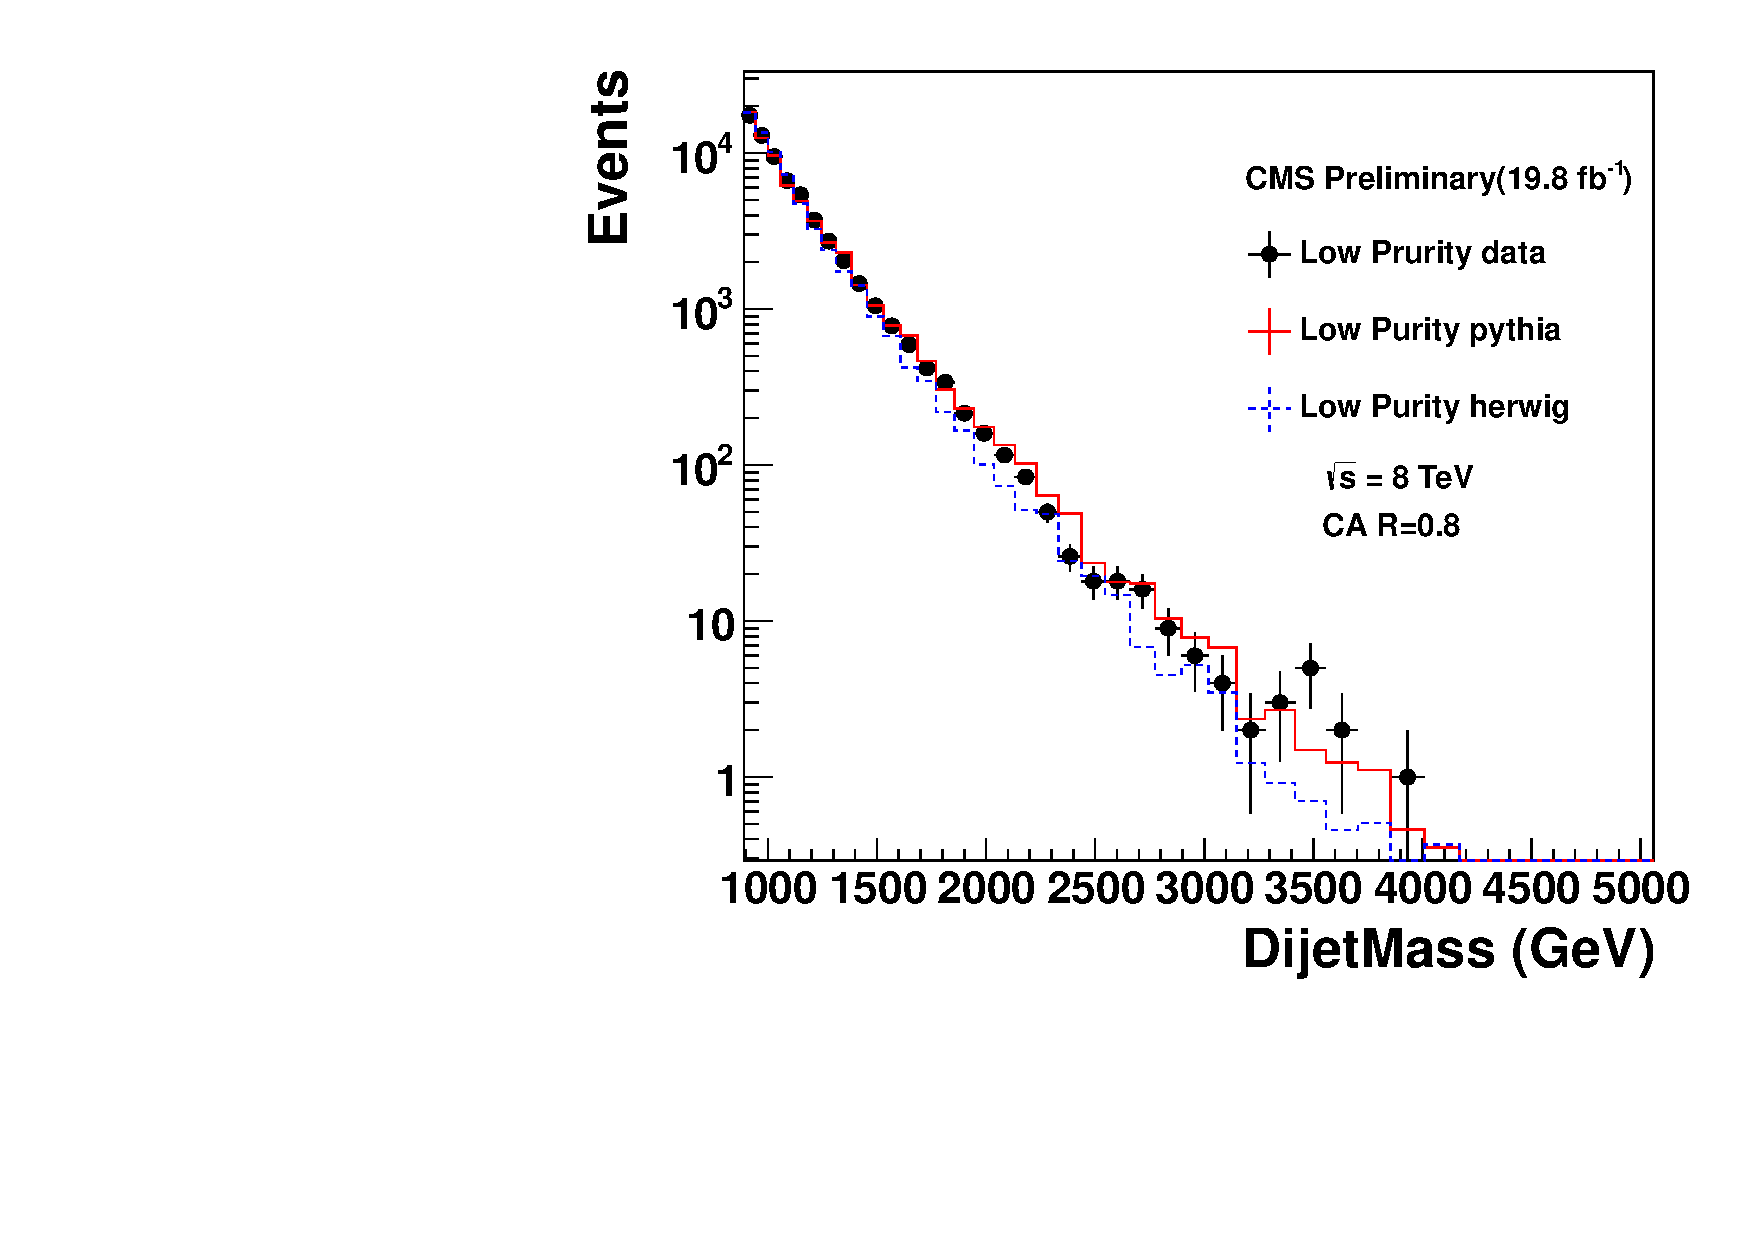
\includegraphics{EXO-12-024/figs/Data-MC-comparisons/DijetMass-qVLowP.pdf}} &
     \resizebox{0.45\linewidth}{!}{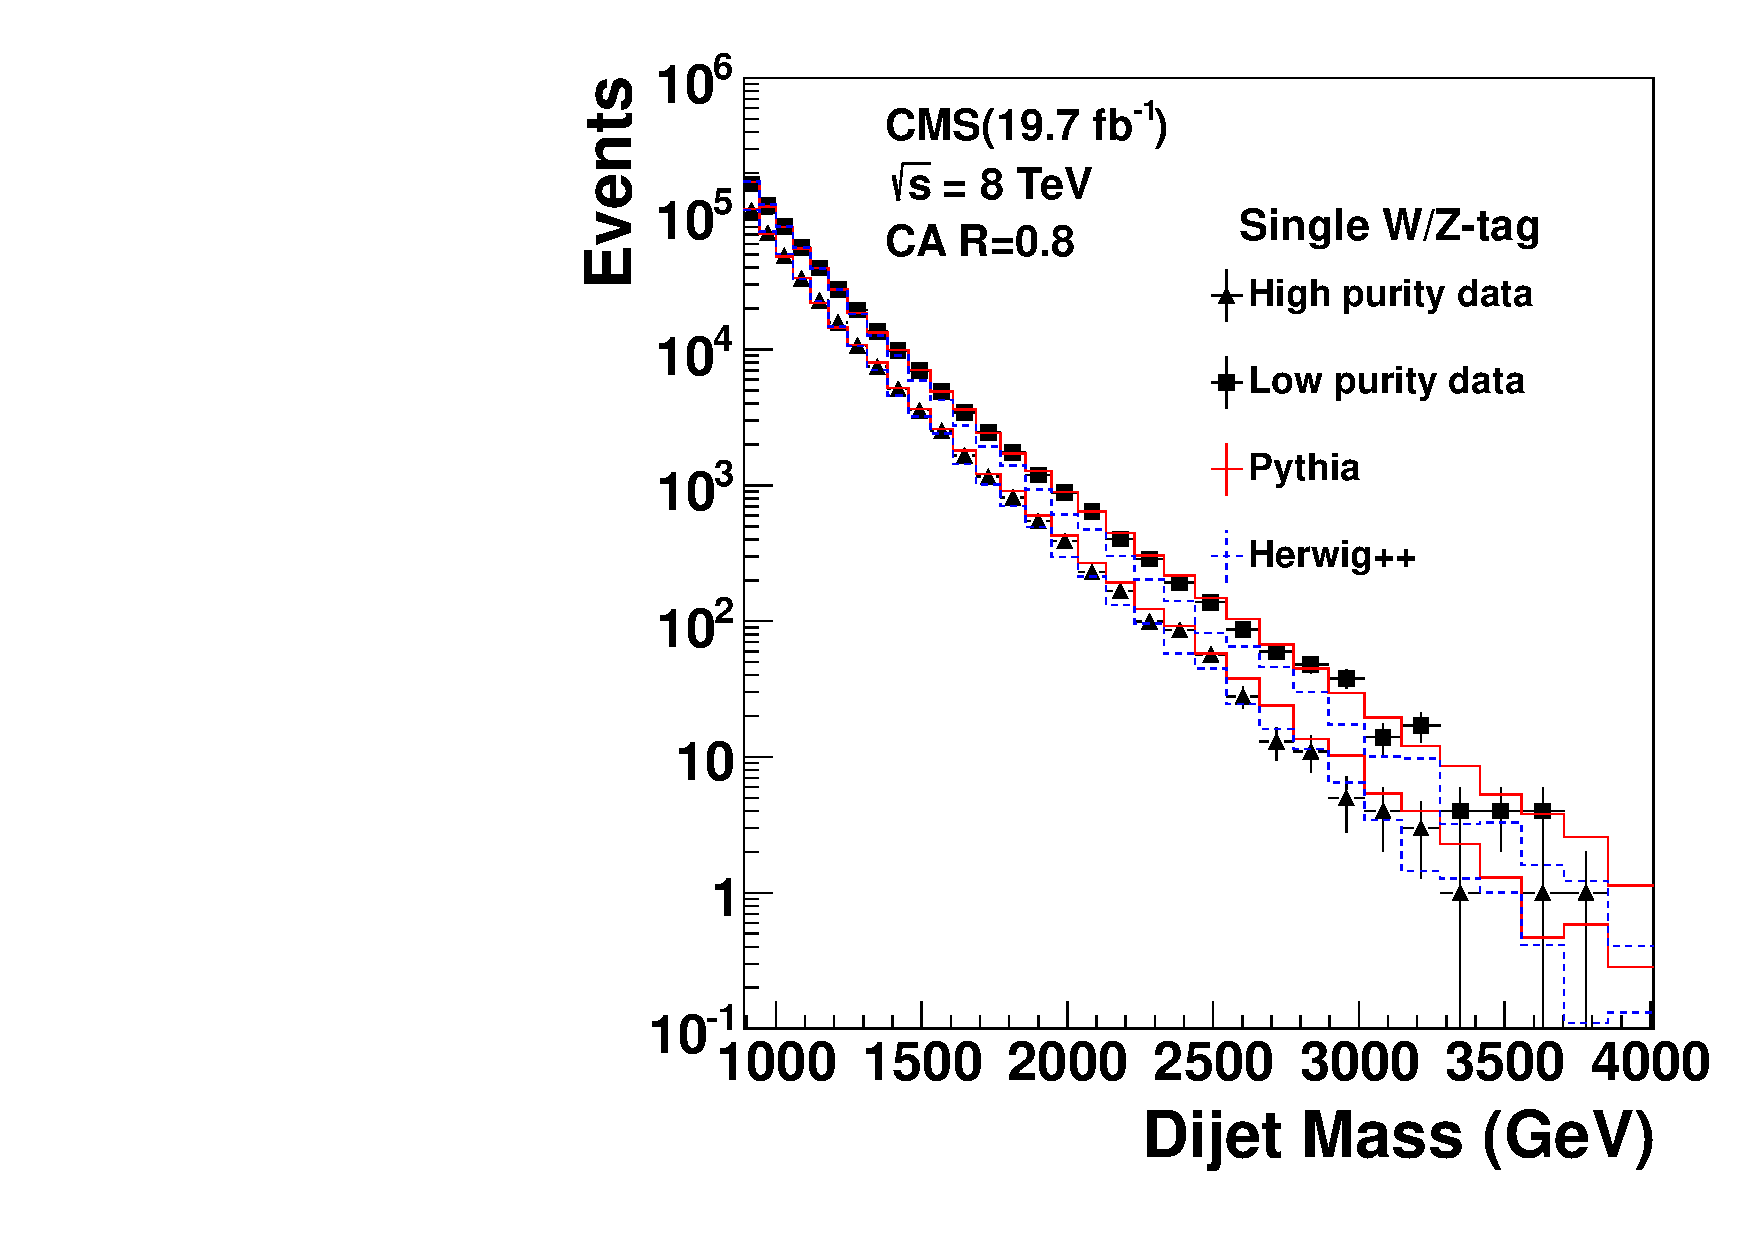
\includegraphics{EXO-12-024/figs/Data-MC-comparisons/DijetMass-qVMiumHigh.pdf}} \\
\end{tabular}
  \caption[Invariant Mass Single]{Comparisons between data and Monte Carlo
           for invariant mass of the two leading jets of low purity (left) and low-high purity (right) 1-tagged events.
           The MC is normalized to the number of data events in each category.
           }
  \label{fig:mjjSingle}
\end{figure}

\begin{figure}[htb]
\centering
\begin{tabular}{cc}
     \resizebox{0.53\linewidth}{!}{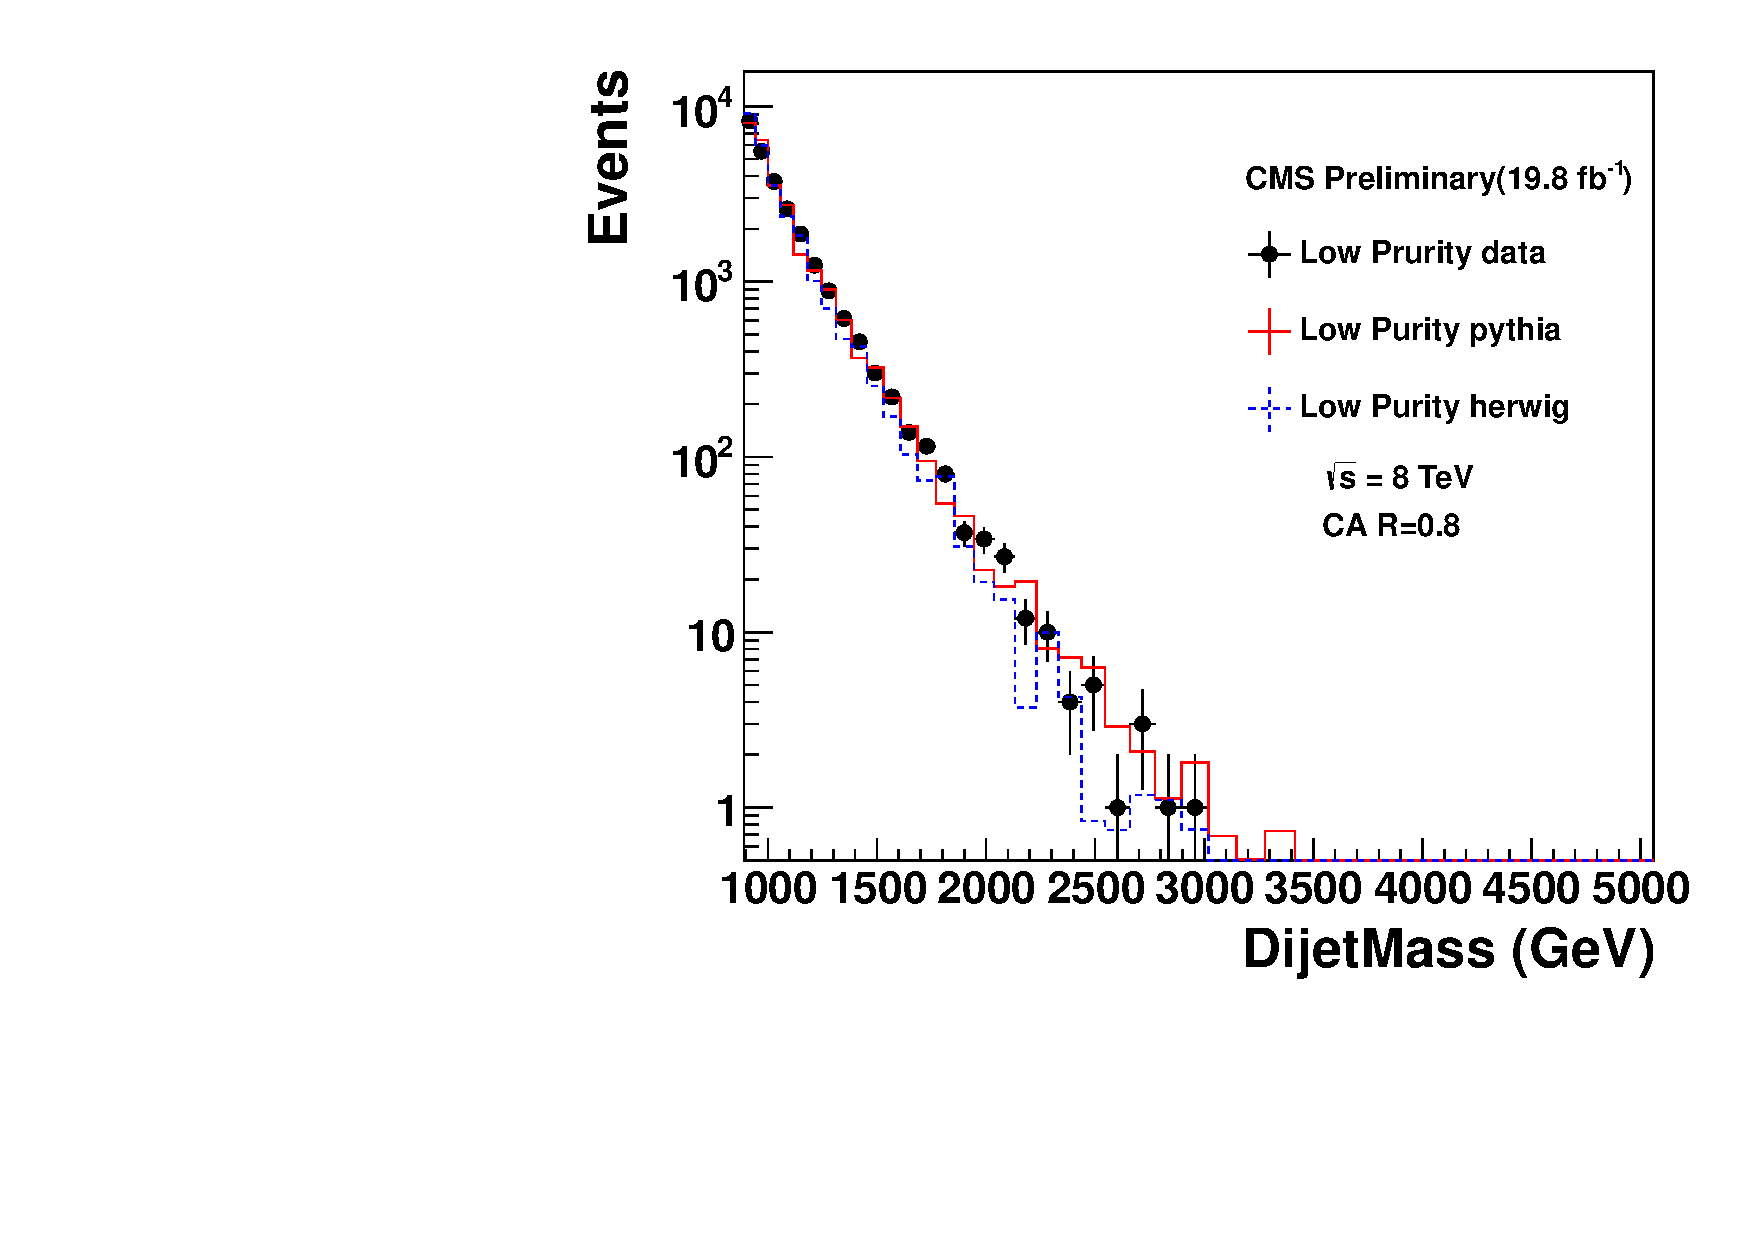
\includegraphics{EXO-12-024/figs/Data-MC-comparisons/DijetMass-VVLowP.pdf}} &
     \resizebox{0.45\linewidth}{!}{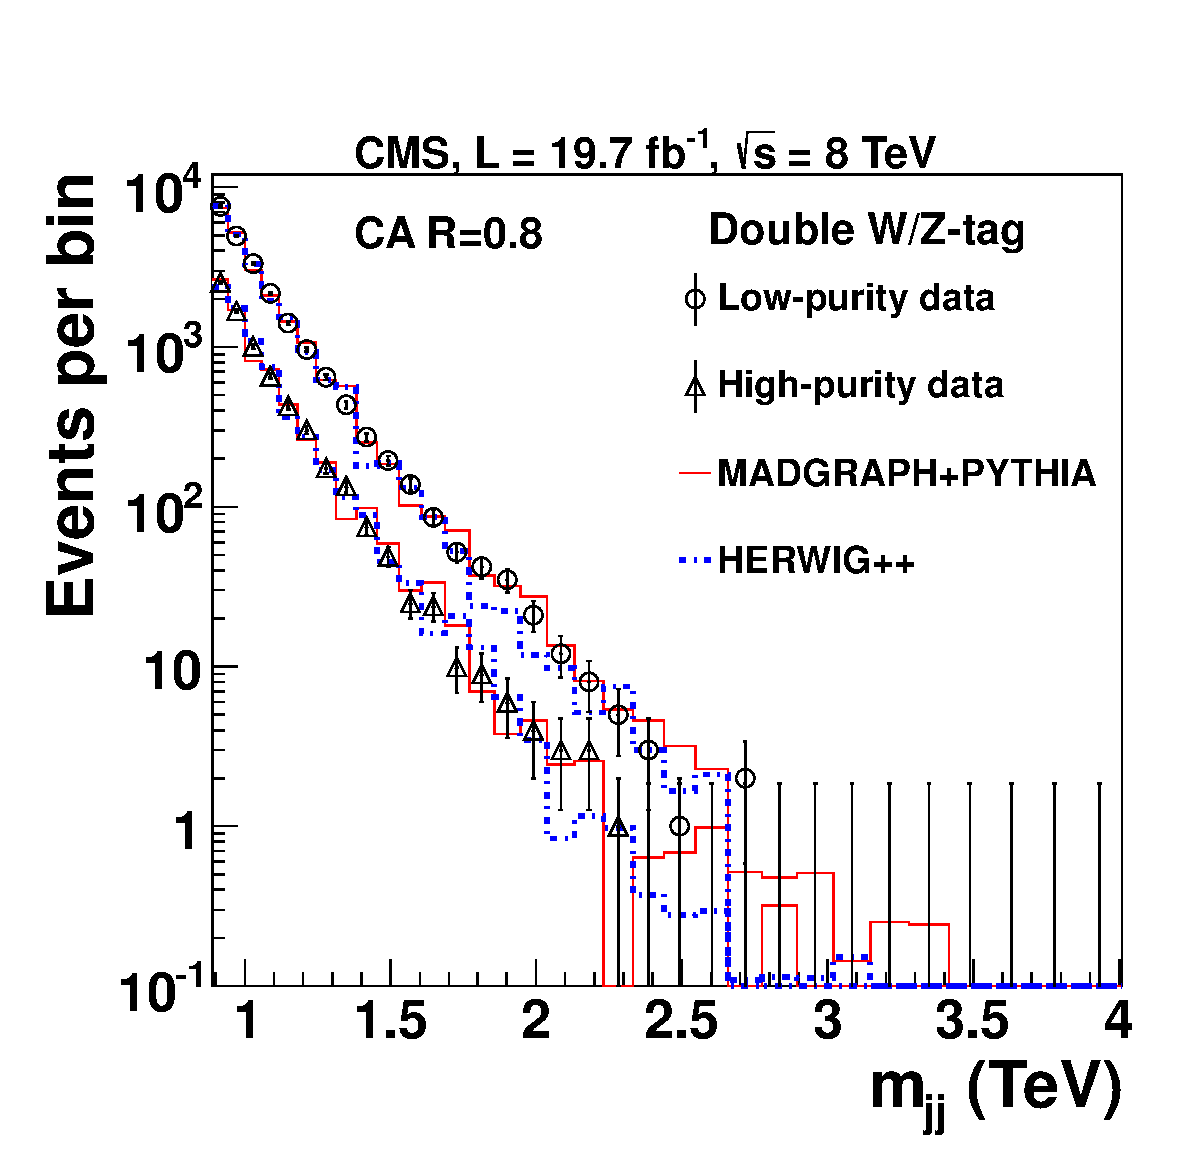
\includegraphics{EXO-12-024/figs/Data-MC-comparisons/DijetMass-VVMiumHigh.pdf}} \\
\end{tabular}
  \caption[Invariant Mass Double]{Comparisons between data and Monte Carlo
           for invariant mass of the two leading jets of low purity (left) and low-high purity (right) 2-tagged events.
           The MC is normalized to the number of data events in each category.
           }
  \label{fig:mjjDouble}
\end{figure}

\newpage
\begin{figure}[htb]
\centering
\begin{tabular}{cc}
     \resizebox{0.5\linewidth}{!}{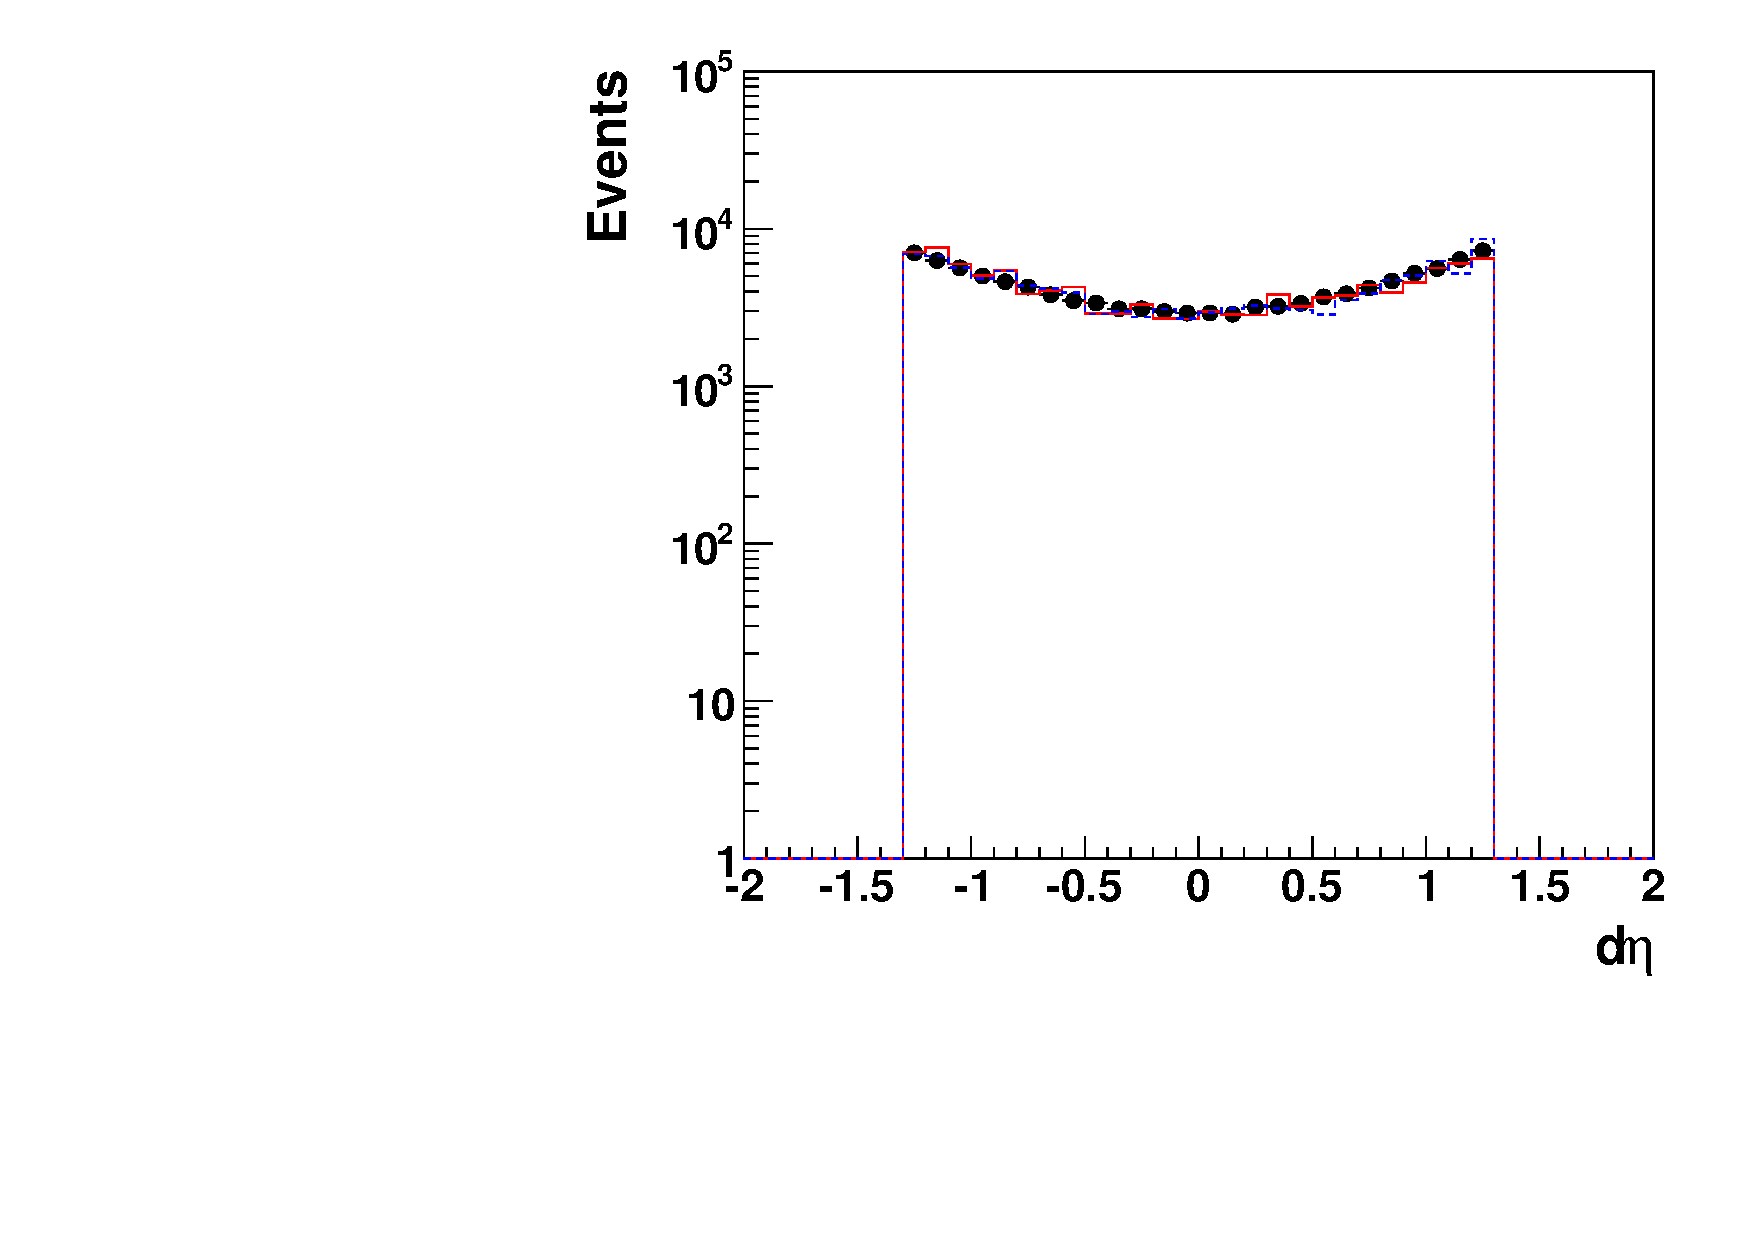
\includegraphics{EXO-12-024/figs/Data-MC-comparisons/Deta-qVLowP.pdf}} &
     \resizebox{0.5\linewidth}{!}{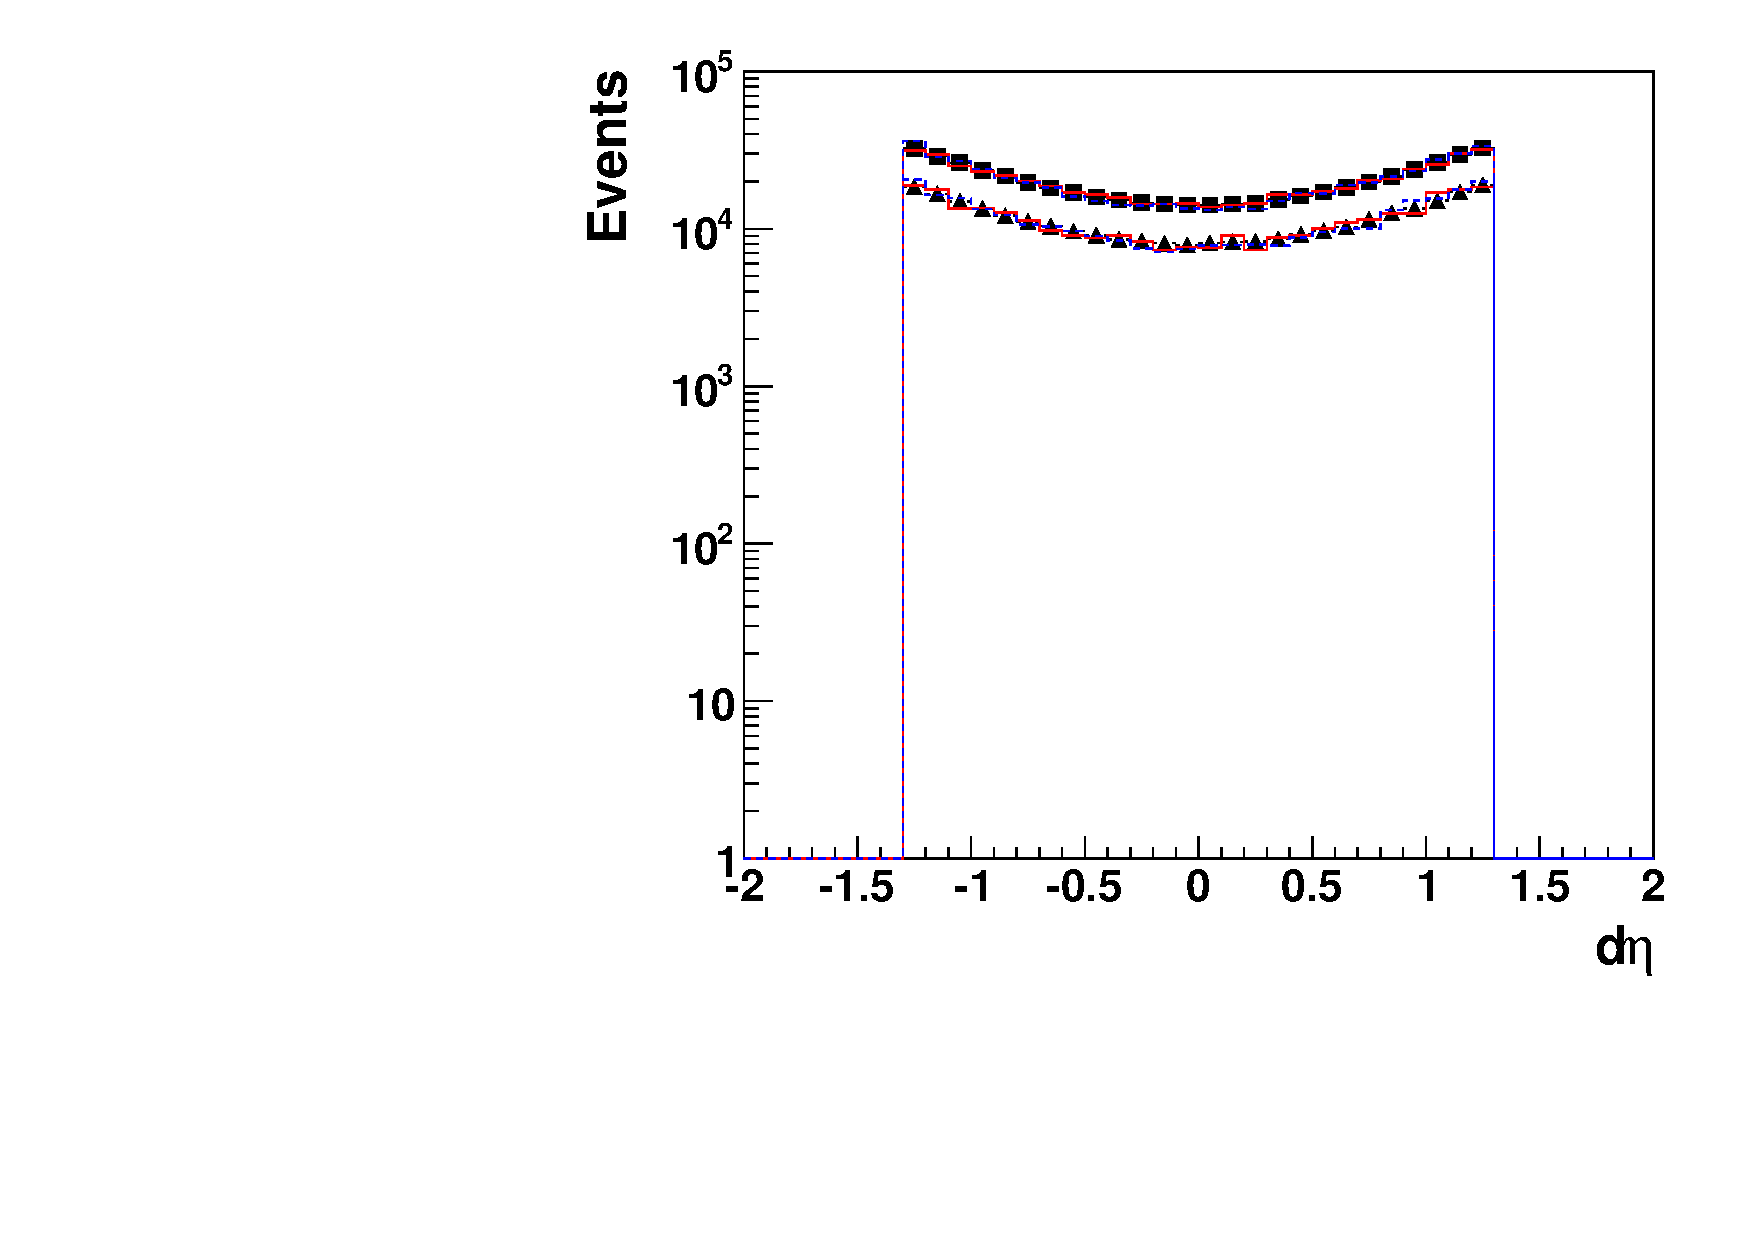
\includegraphics{EXO-12-024/figs/Data-MC-comparisons/Deta-qVMiumHigh.pdf}} \\
\end{tabular}
  \caption[Delta Eta Single]{Comparisons between data and Monte Carlo
                    for $\Delta\eta$ of the two leading jets of low purity (left) and low-high purity (right) 1-tagged events.
	   The MC is normalized to the number of data events in each category. }
  \label{fig:dySingle}
\end{figure}

\begin{figure}[htb]
\centering
\begin{tabular}{cc}
     \resizebox{0.5\linewidth}{!}{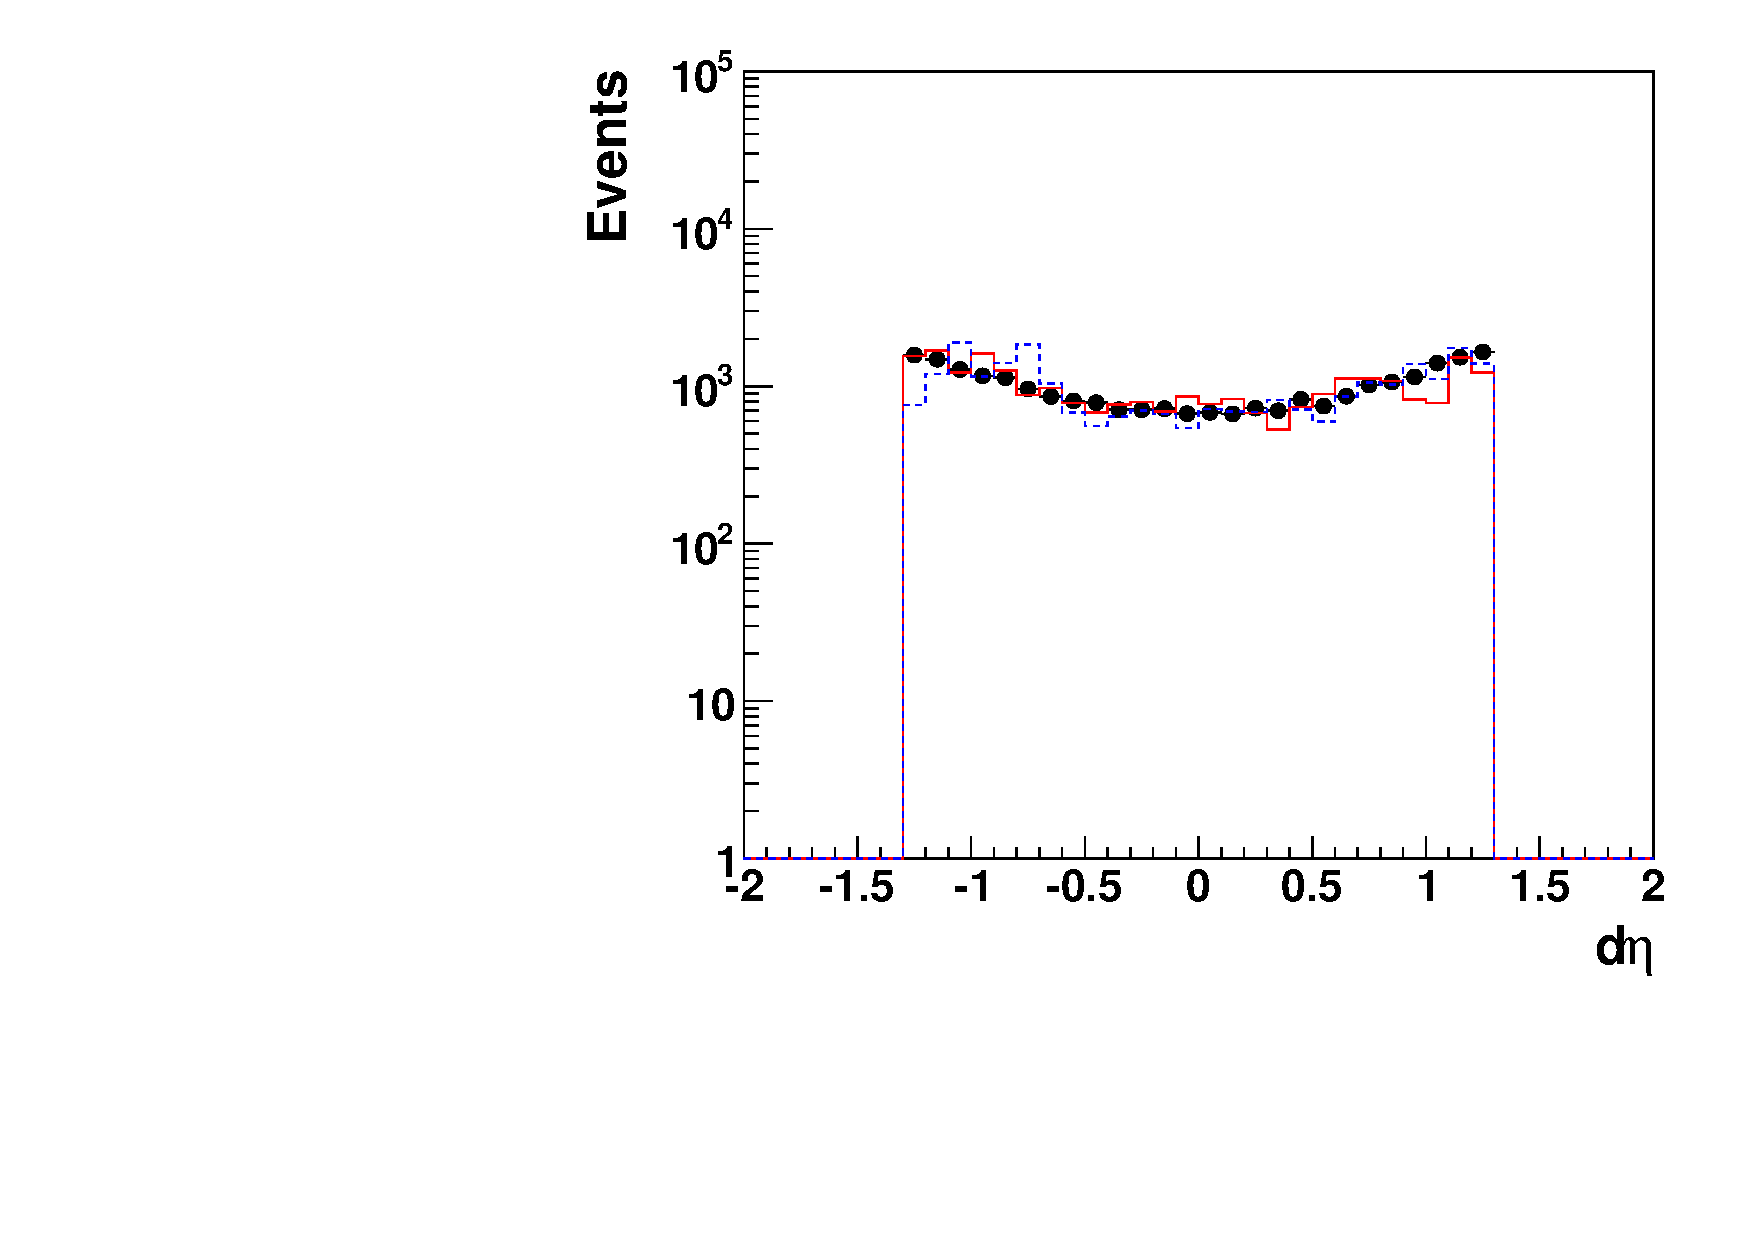
\includegraphics{EXO-12-024/figs/Data-MC-comparisons/Deta-VVLowP.pdf}} &
     \resizebox{0.5\linewidth}{!}{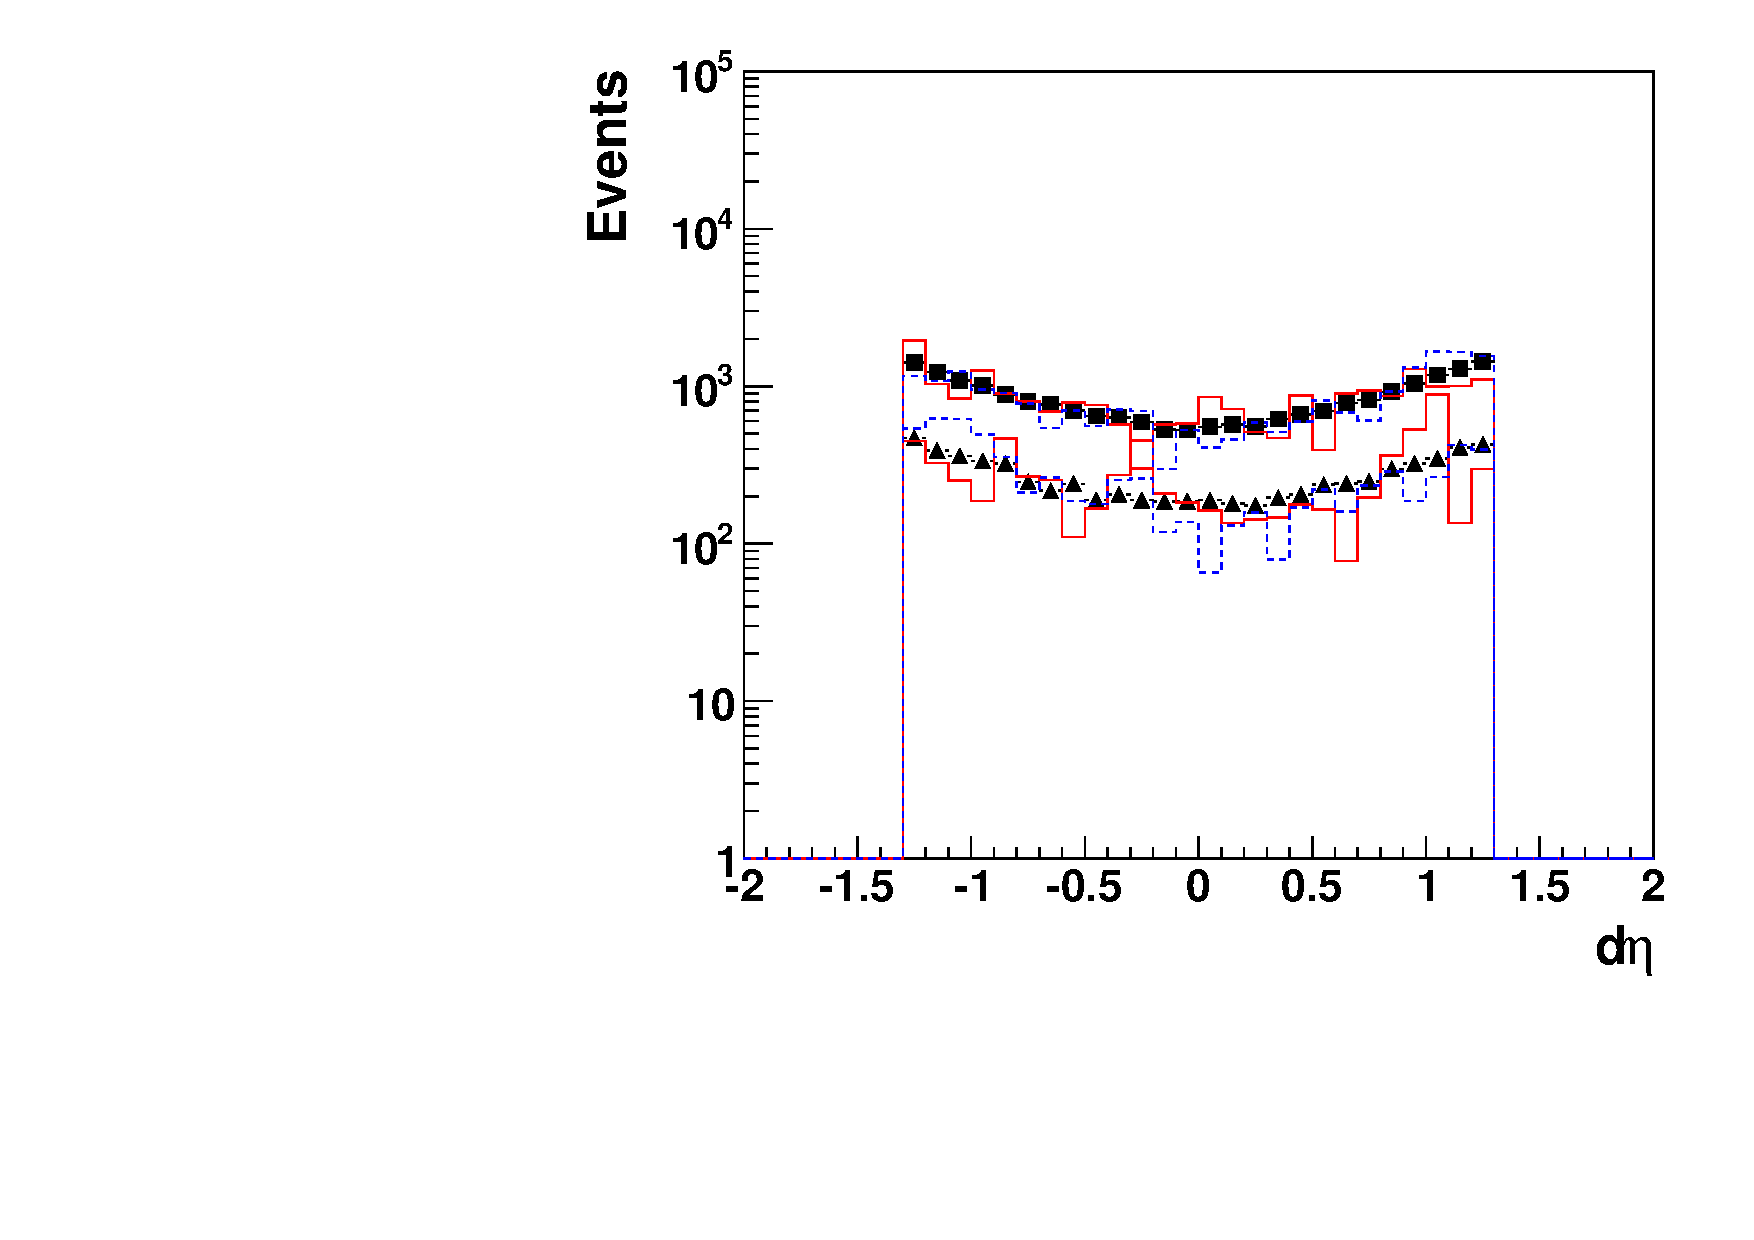
\includegraphics{EXO-12-024/figs/Data-MC-comparisons/Deta-VVMiumHigh.pdf}} \\
\end{tabular}
  \caption[Delta Eta Double]{Comparisons between data and Monte Carlo
                     for $\Delta\eta$ of the two leading jets of low purity (left) and low-high purity (right) 2-tagged events. The MC is normalized to the number of data events in each category. }
  \label{fig:dyDouble}
\end{figure}


\newpage
\begin{figure}[htb]
\centering
\begin{tabular}{cc}
     \resizebox{0.5\linewidth}{!}{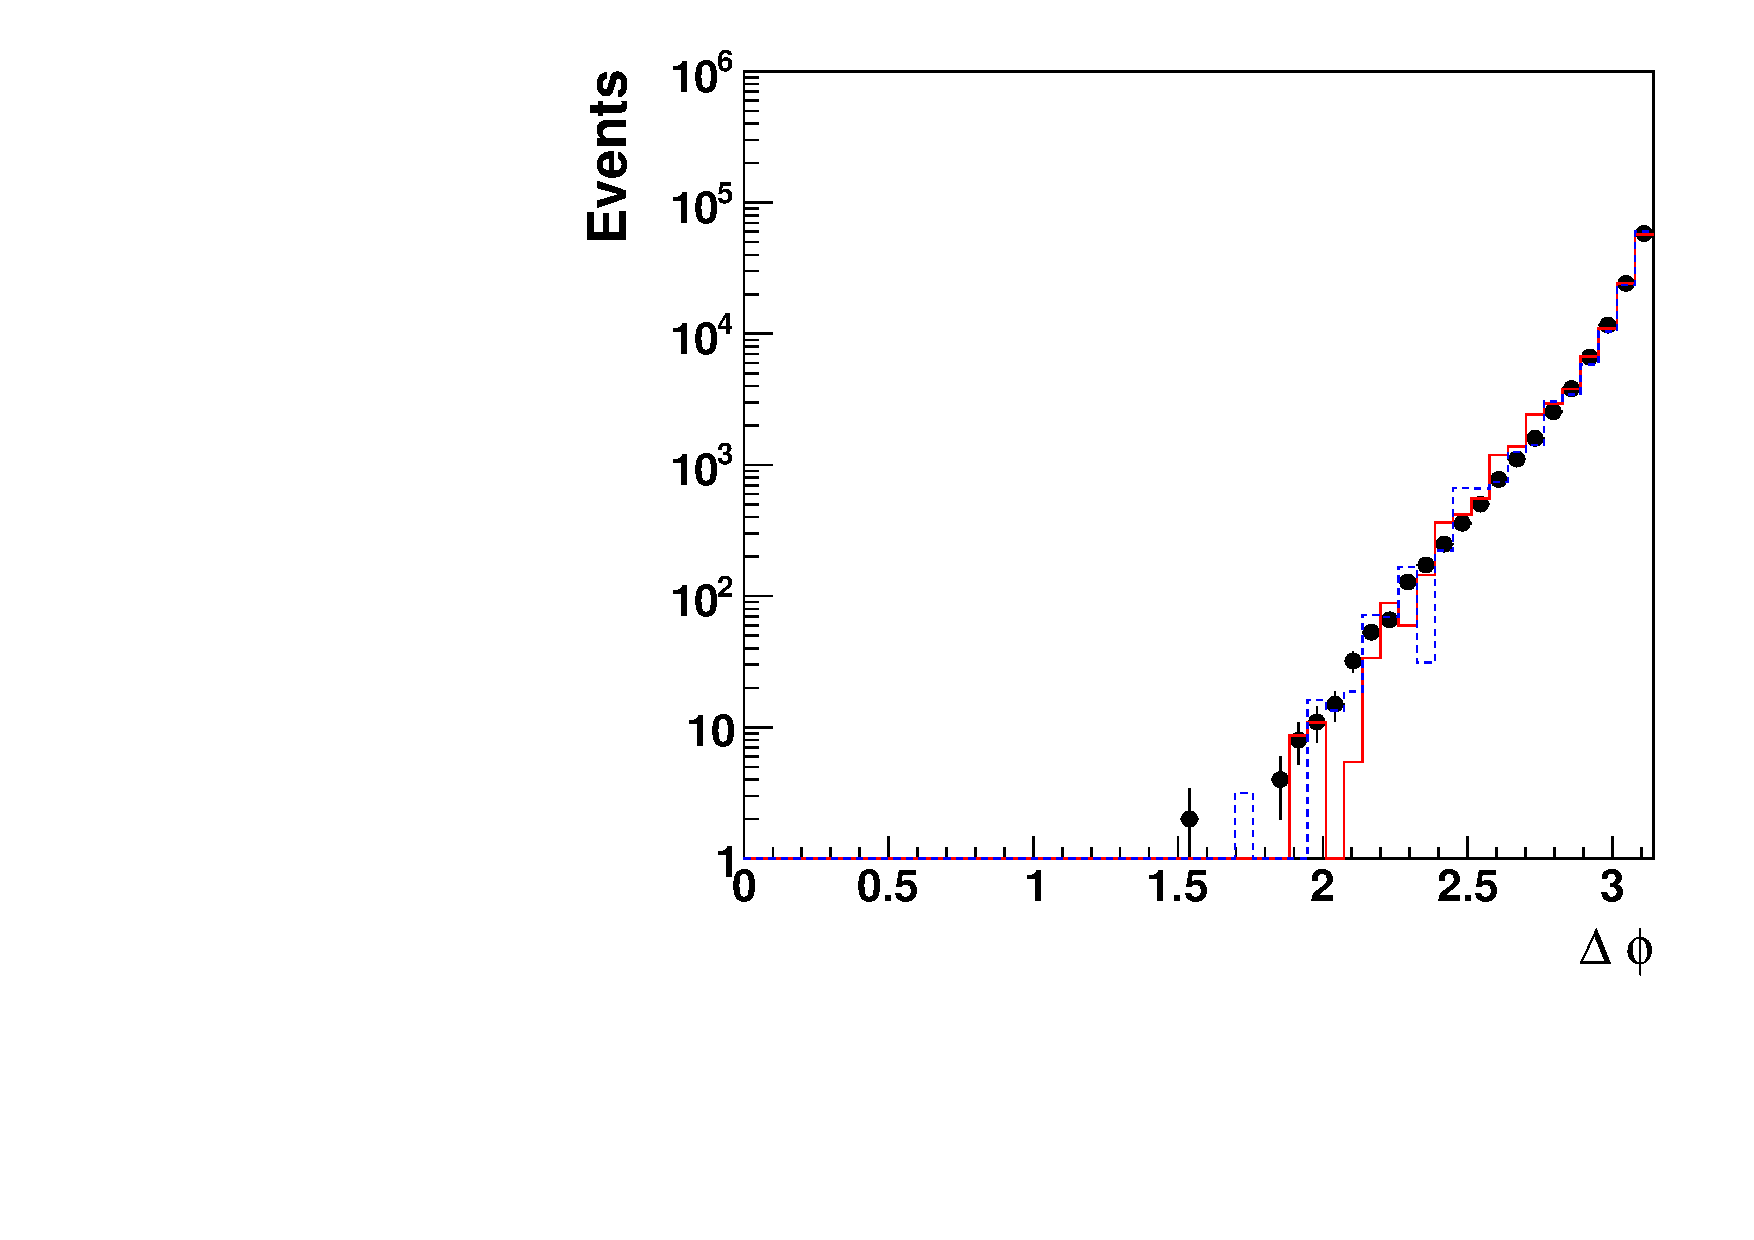
\includegraphics{EXO-12-024/figs/Data-MC-comparisons/Dphi-qVLowP.pdf}} &
     \resizebox{0.5\linewidth}{!}{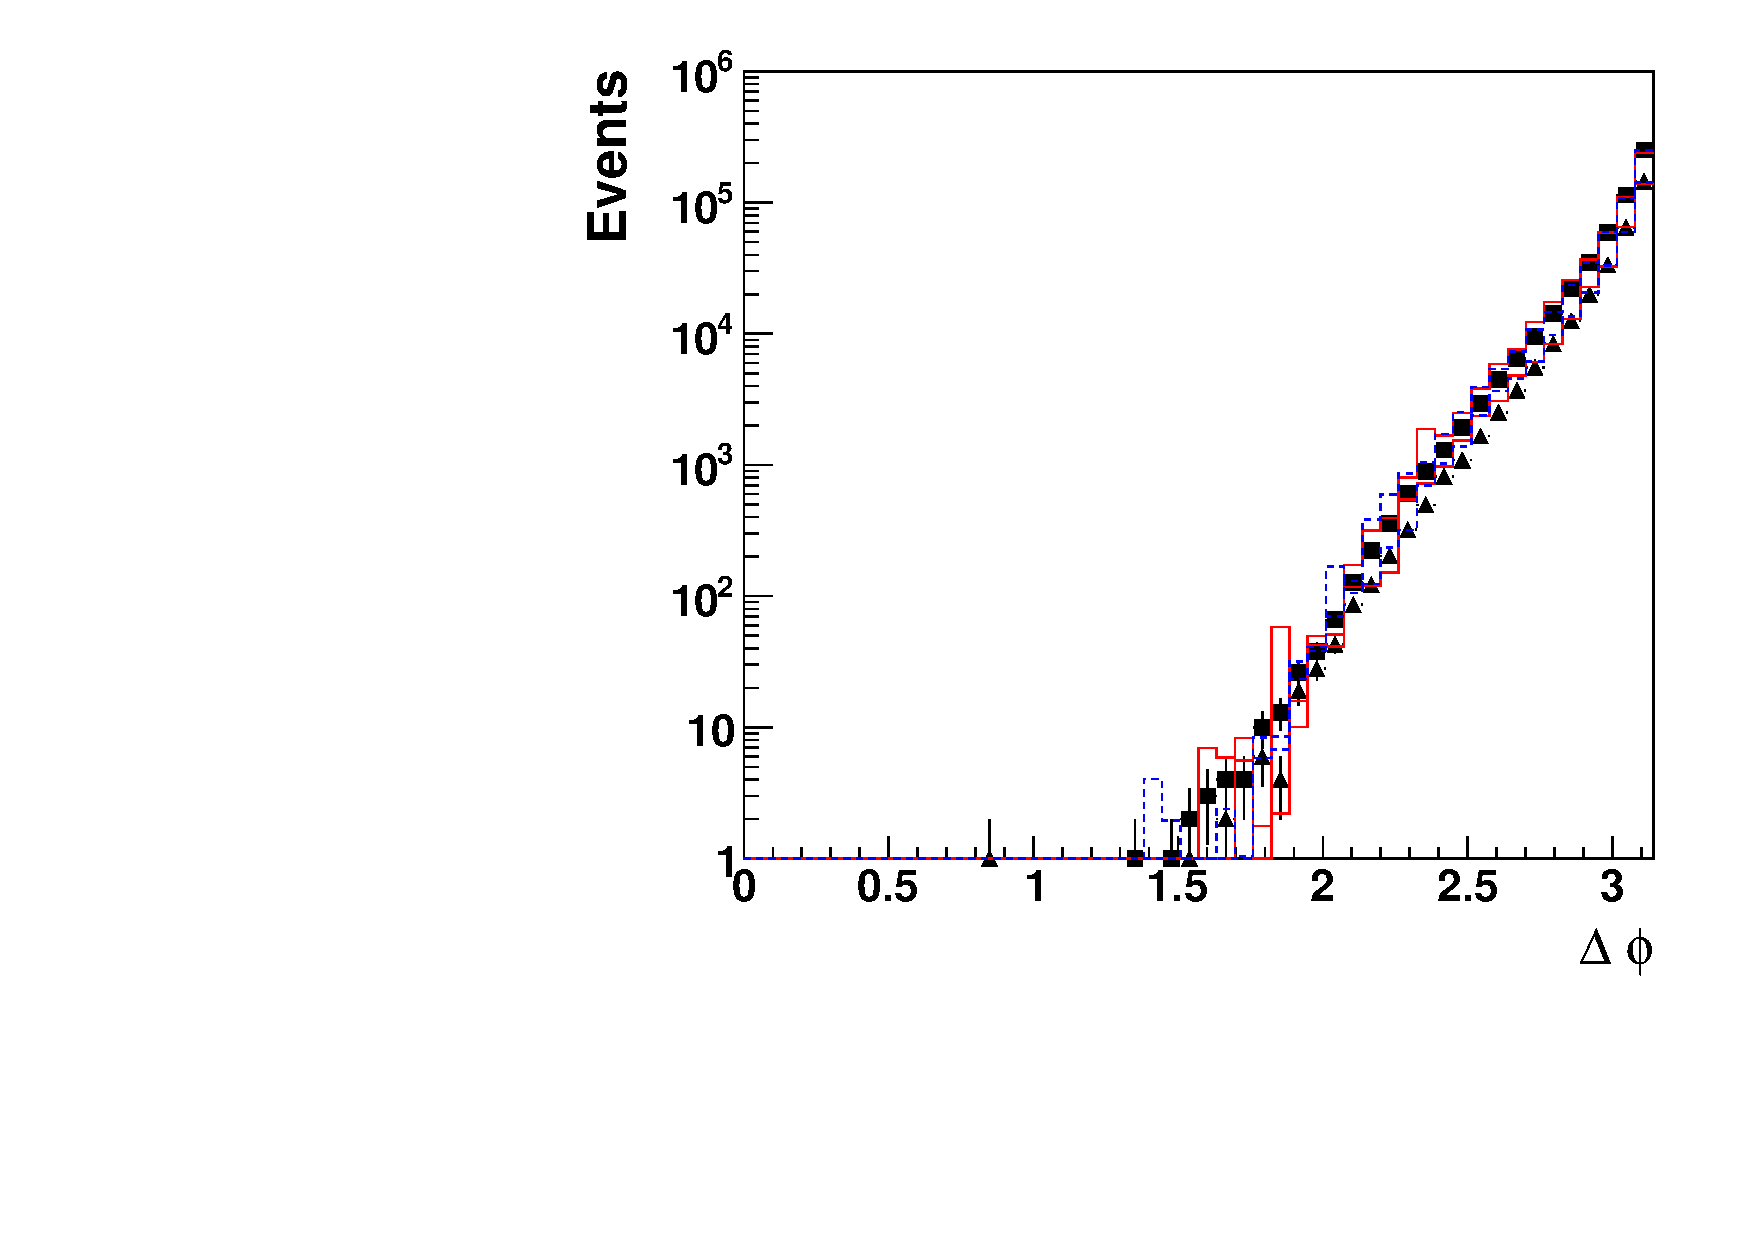
\includegraphics{EXO-12-024/figs/Data-MC-comparisons/Dphi-qVMiumHigh.pdf}} \\
\end{tabular}
  \caption[Delta Eta Single]{Comparisons between data and Monte Carlo
                    for $\Delta\phi$ of the two leading jets of low purity (left) and low-high purity (right) 1-tagged events.
	   The MC is normalized to the number of data events in each category. }
  \label{fig:dphiSingle}
\end{figure}

\begin{figure}[htb]
\centering
\begin{tabular}{cc}
     \resizebox{0.5\linewidth}{!}{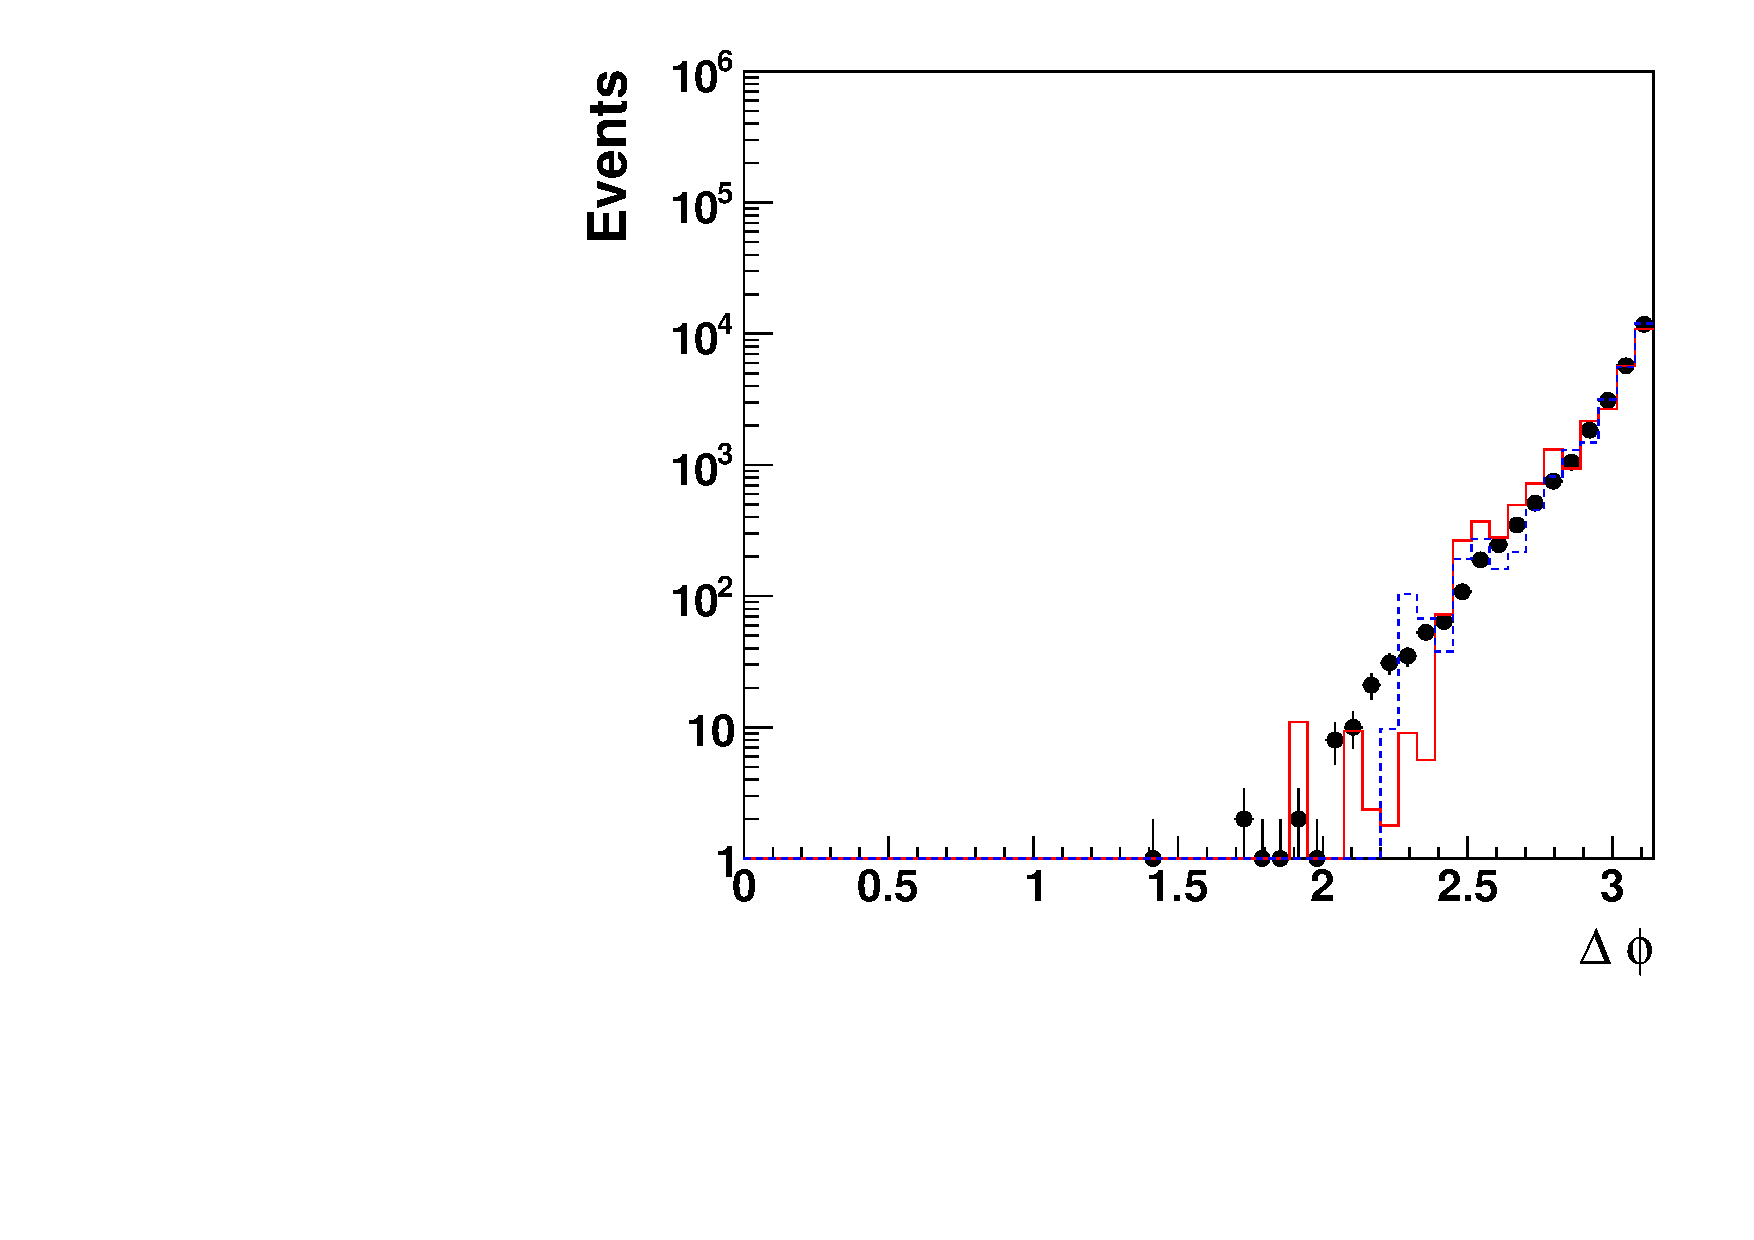
\includegraphics{EXO-12-024/figs/Data-MC-comparisons/Dphi-VVLowP.pdf}} &
     \resizebox{0.5\linewidth}{!}{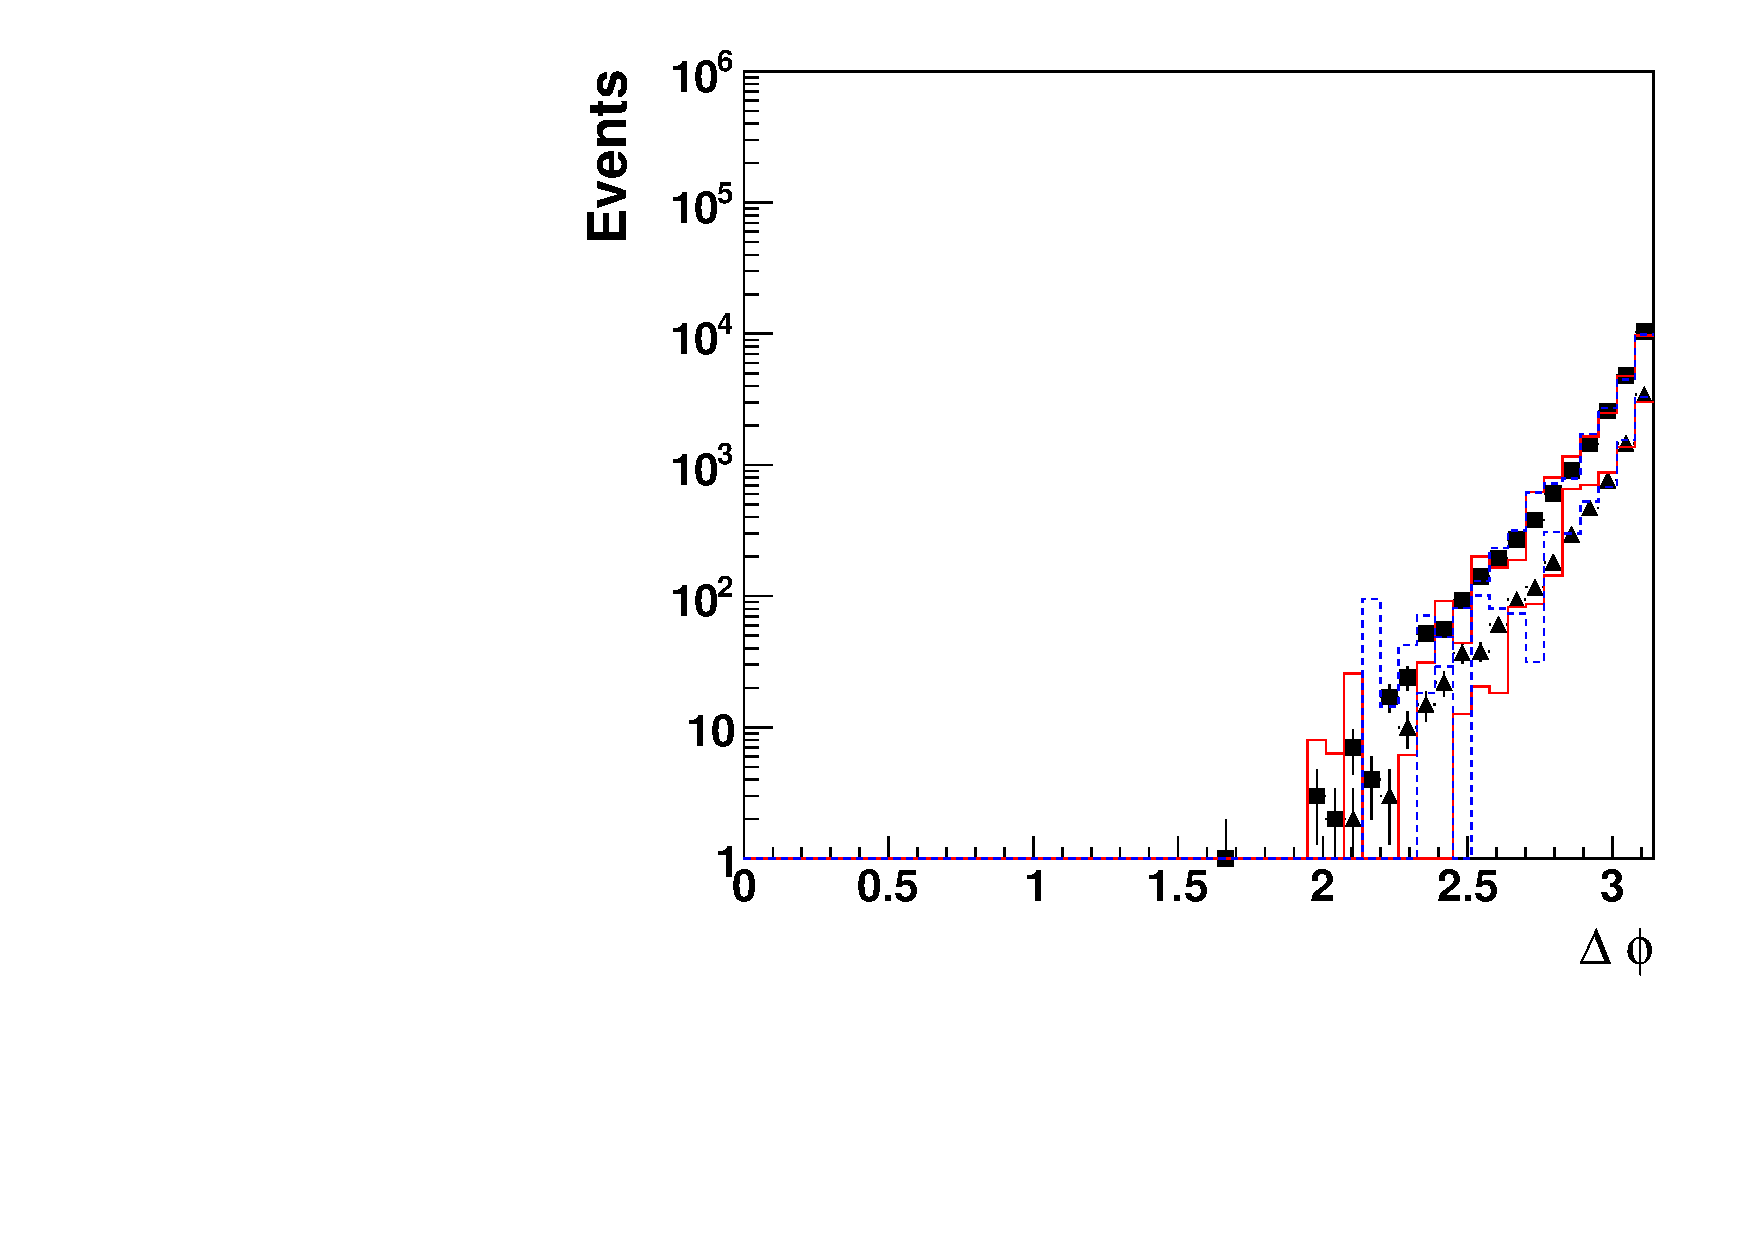
\includegraphics{EXO-12-024/figs/Data-MC-comparisons/Dphi-VVMiumHigh.pdf}} \\
\end{tabular}
  \caption[Delta Eta Double]{Comparisons between data and Monte Carlo
                     for $\Delta\phi$ of the two leading jets of low purity (left) and low-high purity (right) 2-tagged events. The MC is normalized to the number of data events in each category. }
  \label{fig:dphiDouble}
\end{figure}

\newpage

\begin{figure}[htb]
\centering
\begin{tabular}{cc}
     \resizebox{0.5\linewidth}{!}{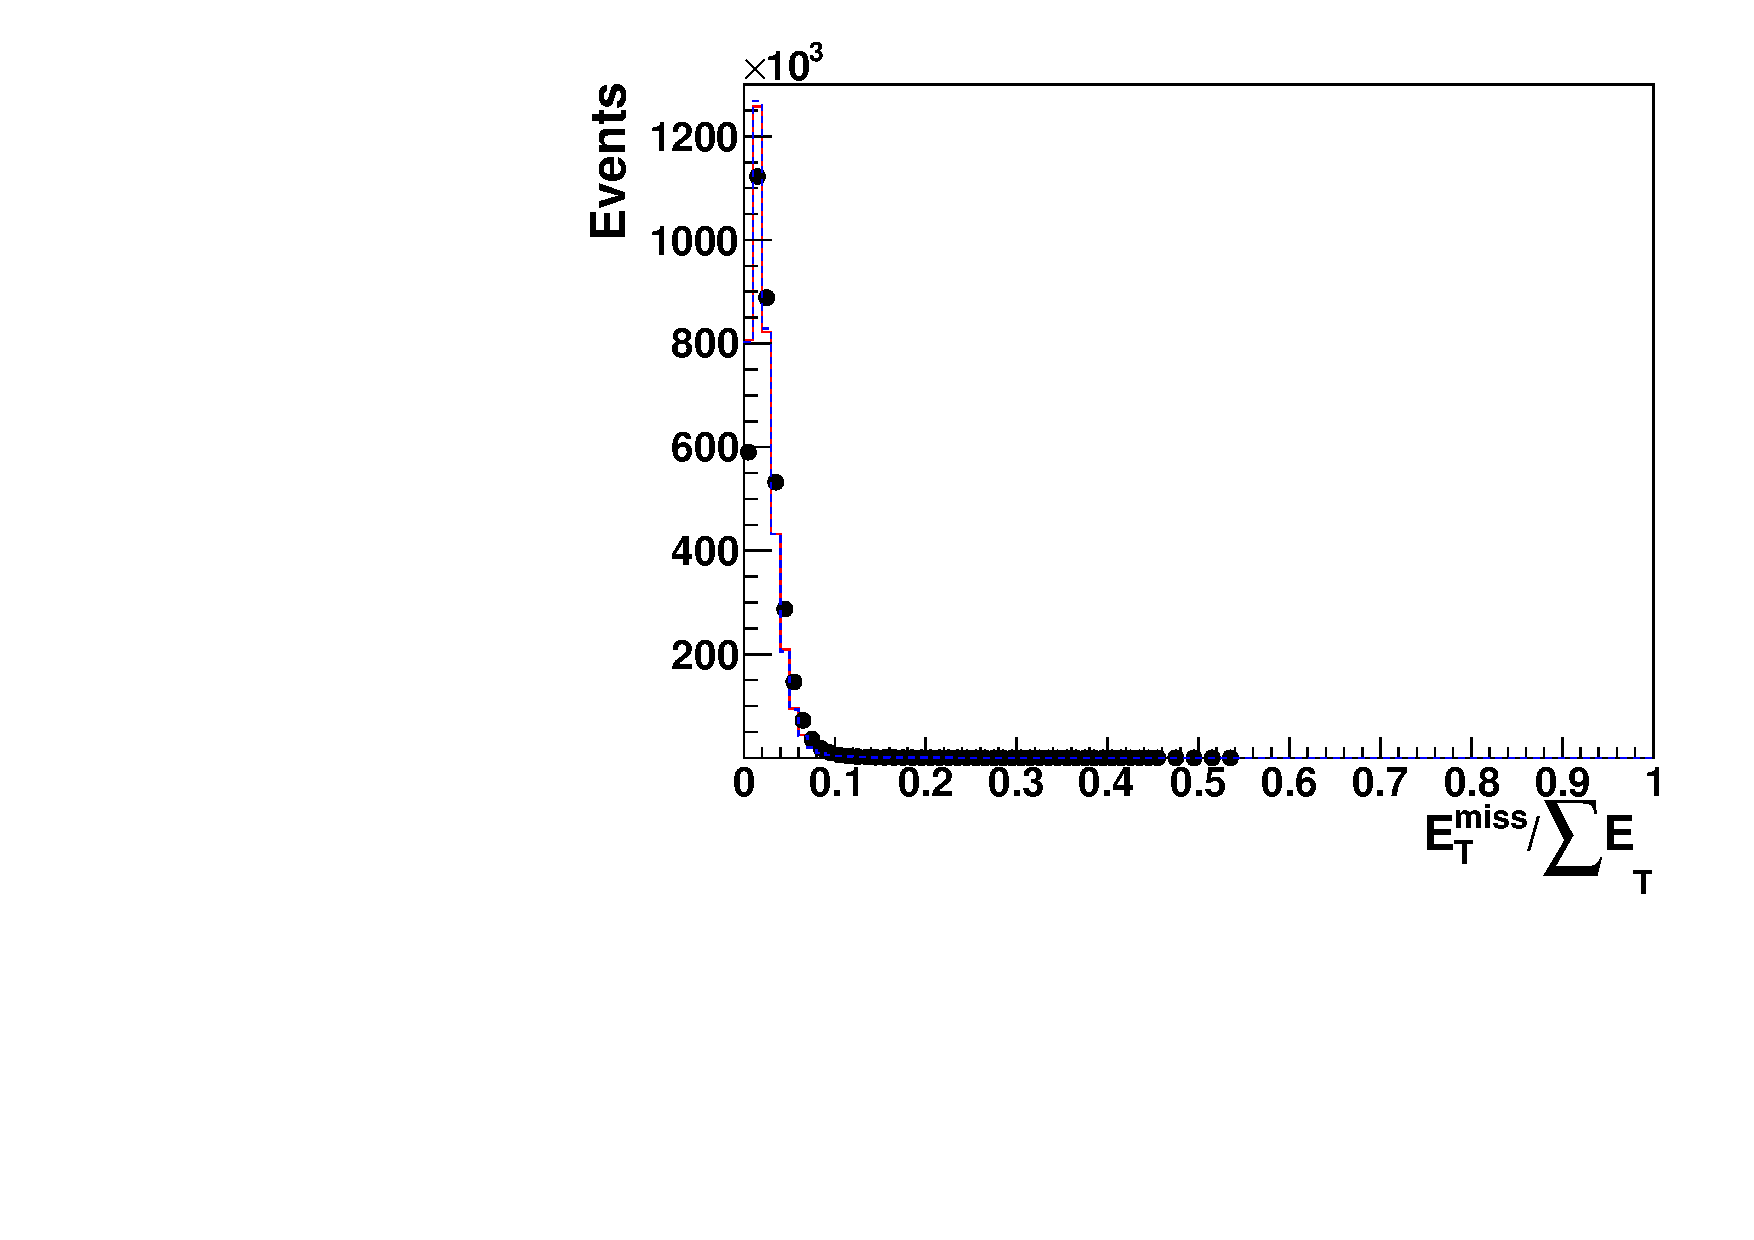
\includegraphics{EXO-12-024/figs/Data-MC-comparisons/etsumEt.pdf}} &
     \resizebox{0.5\linewidth}{!}{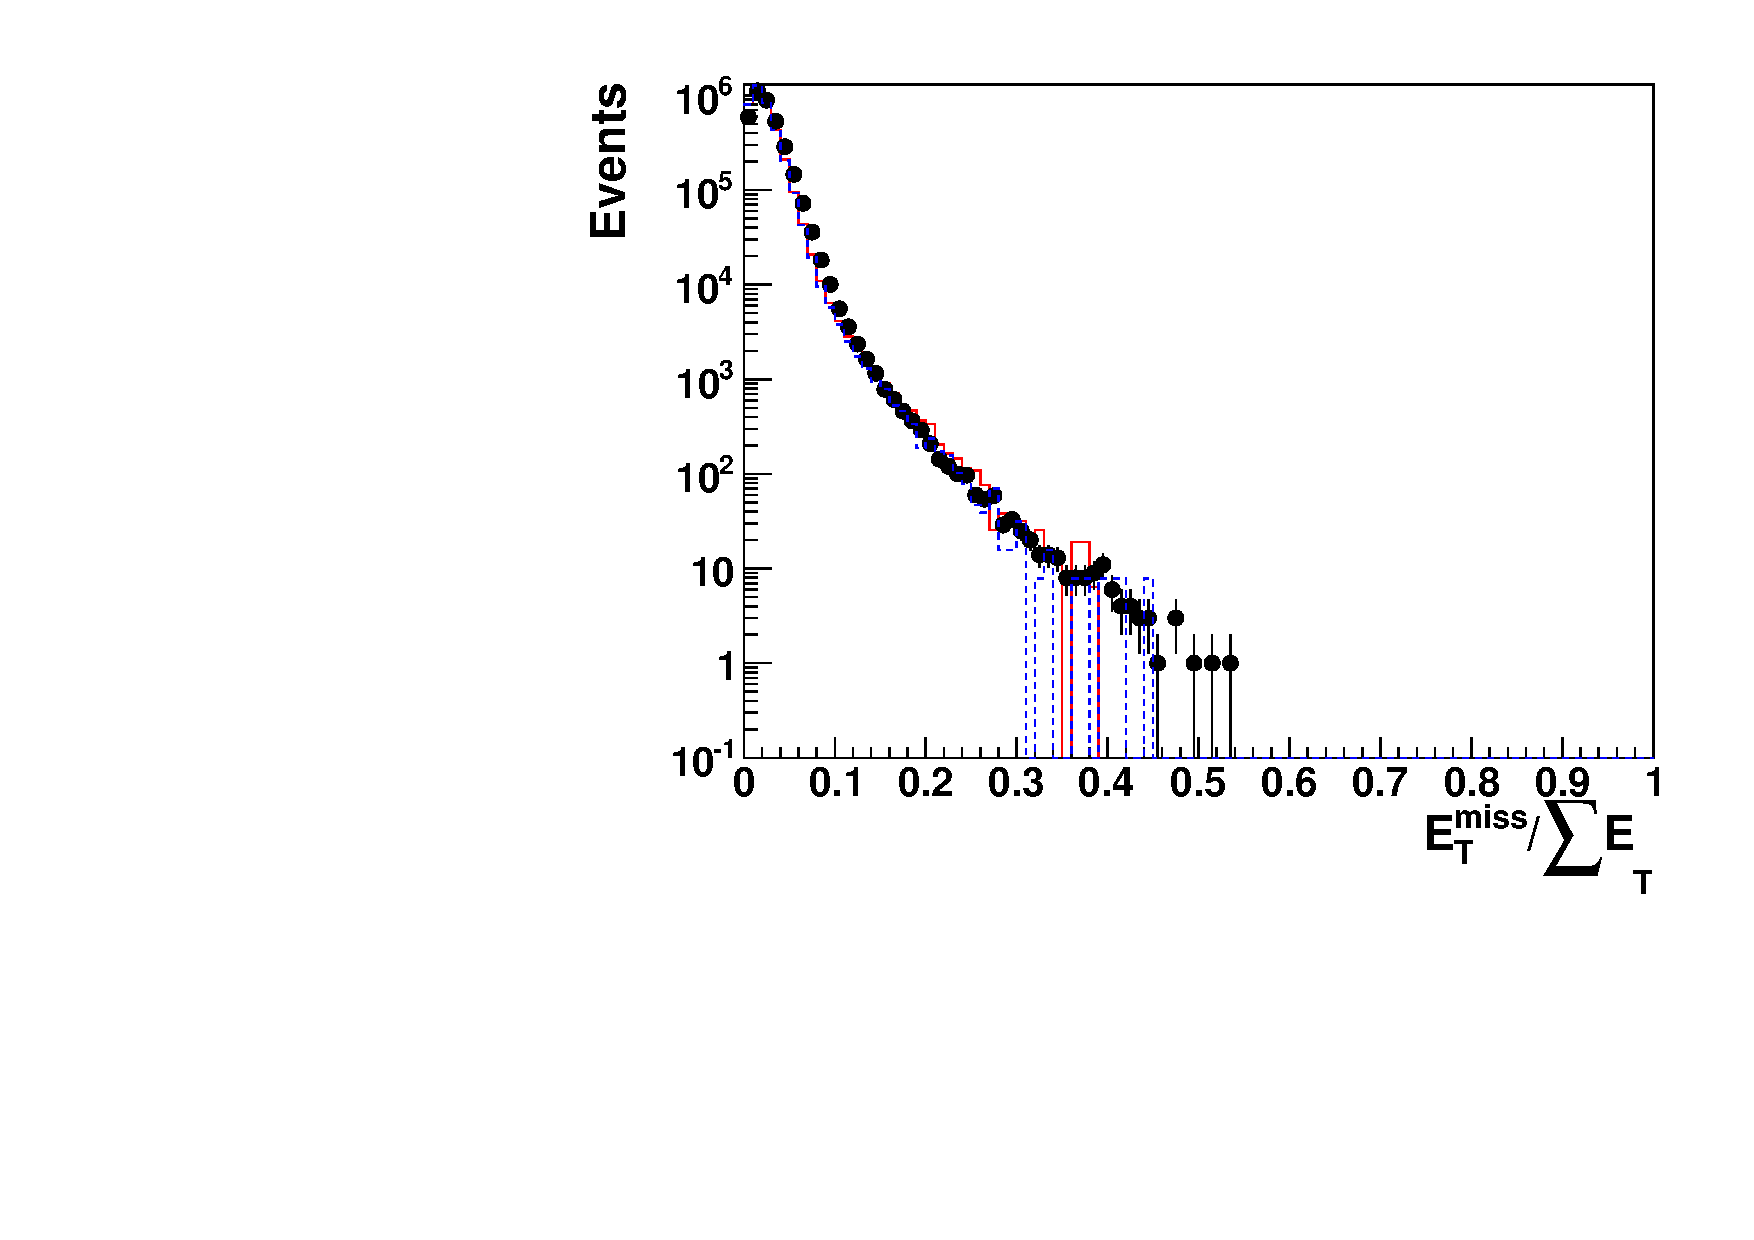
\includegraphics{EXO-12-024/figs/Data-MC-comparisons/etsumEtlog.pdf}} \\
\end{tabular}
  \caption[Leading two jets mass drop]{Comparisons between data and Monte Carlo for $E_{T}^{miss}/\sum E_{T}$ 
	   The MC is normalized to the number of data events. Plot on the right is the log scale plot. (The plot includes only a subset of the full data sample.)}
  \label{fig:metSumPtSingle}
\end{figure}

%\begin{figure}[htb]
%\centering
%\begin{tabular}{cc}
%     \resizebox{0.5\linewidth}{!}{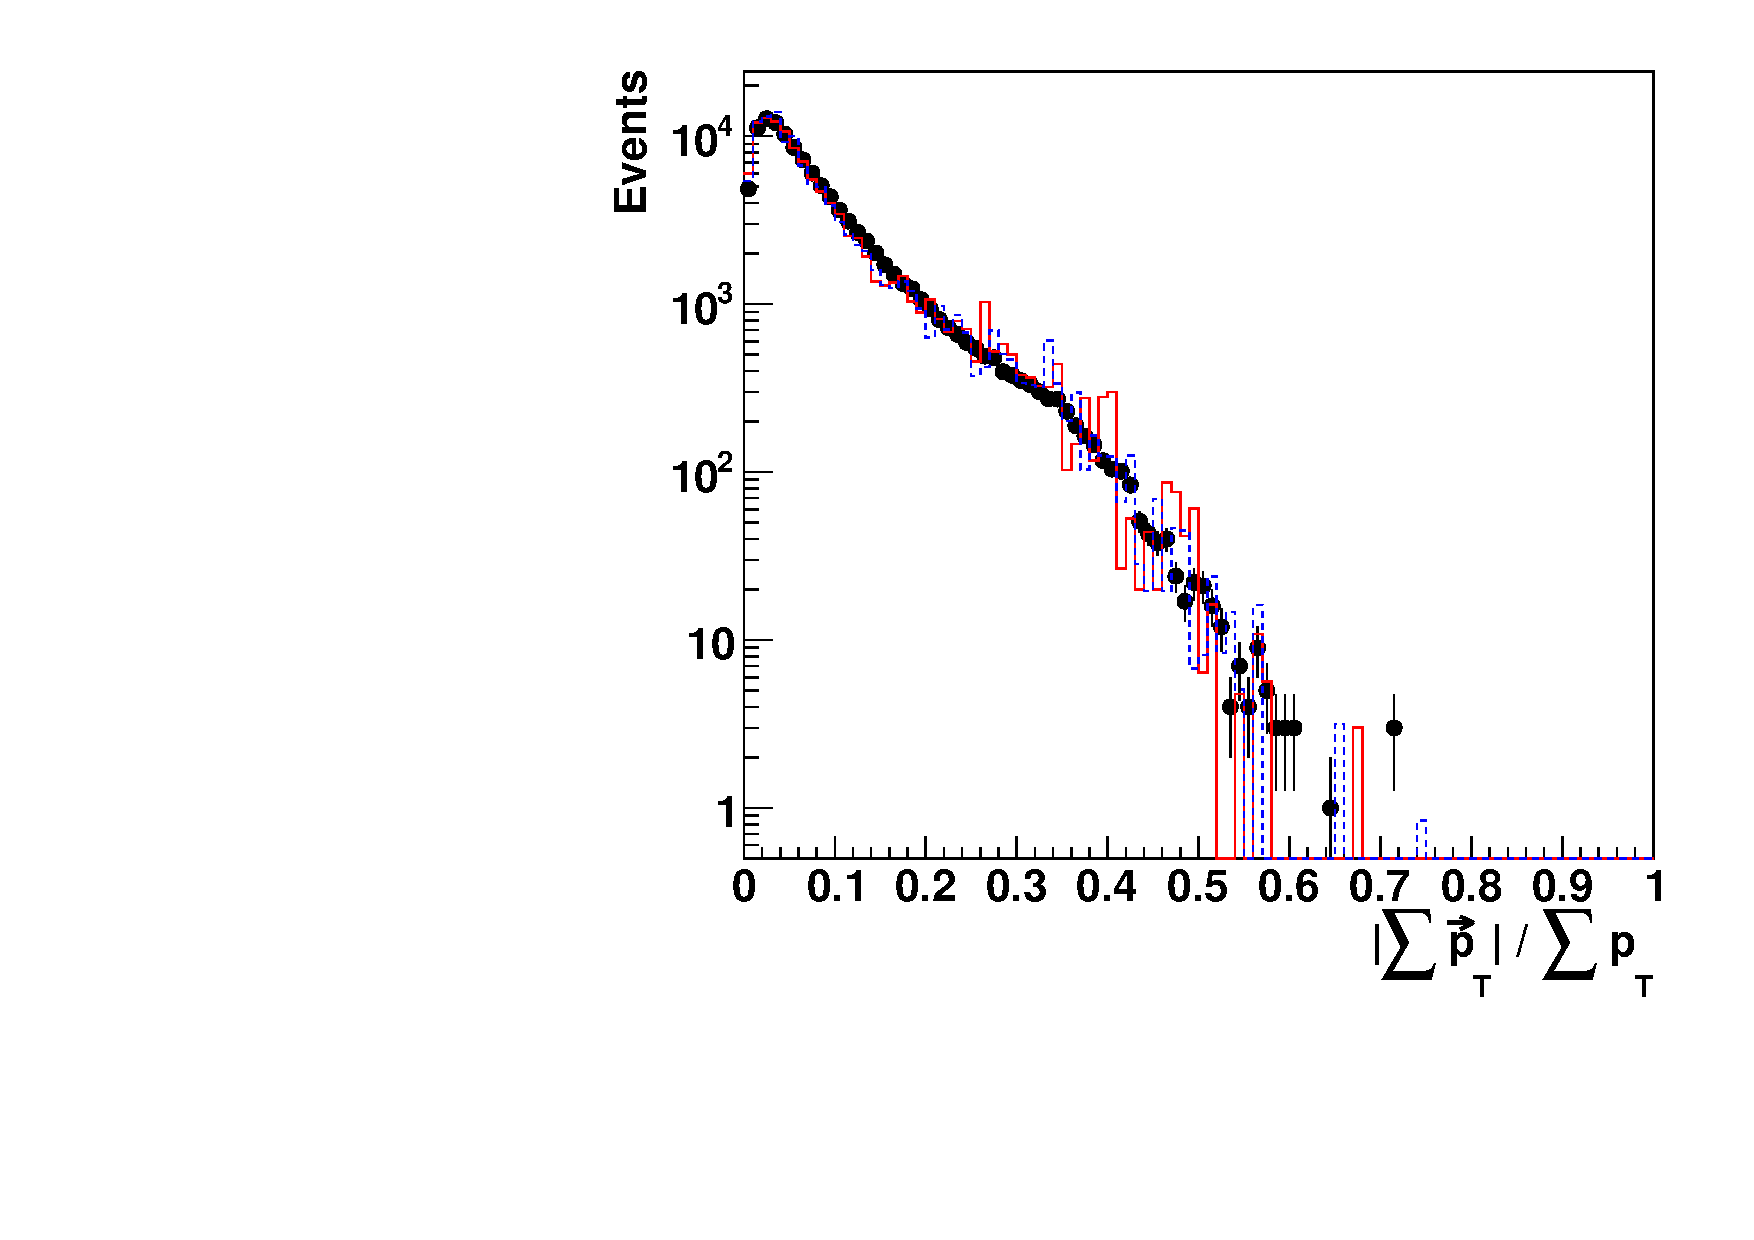
\includegraphics{EXO-12-024/figs/Data-MC-comparisons/PTVSPT-qVLowP.pdf}} &
%     \resizebox{0.5\linewidth}{!}{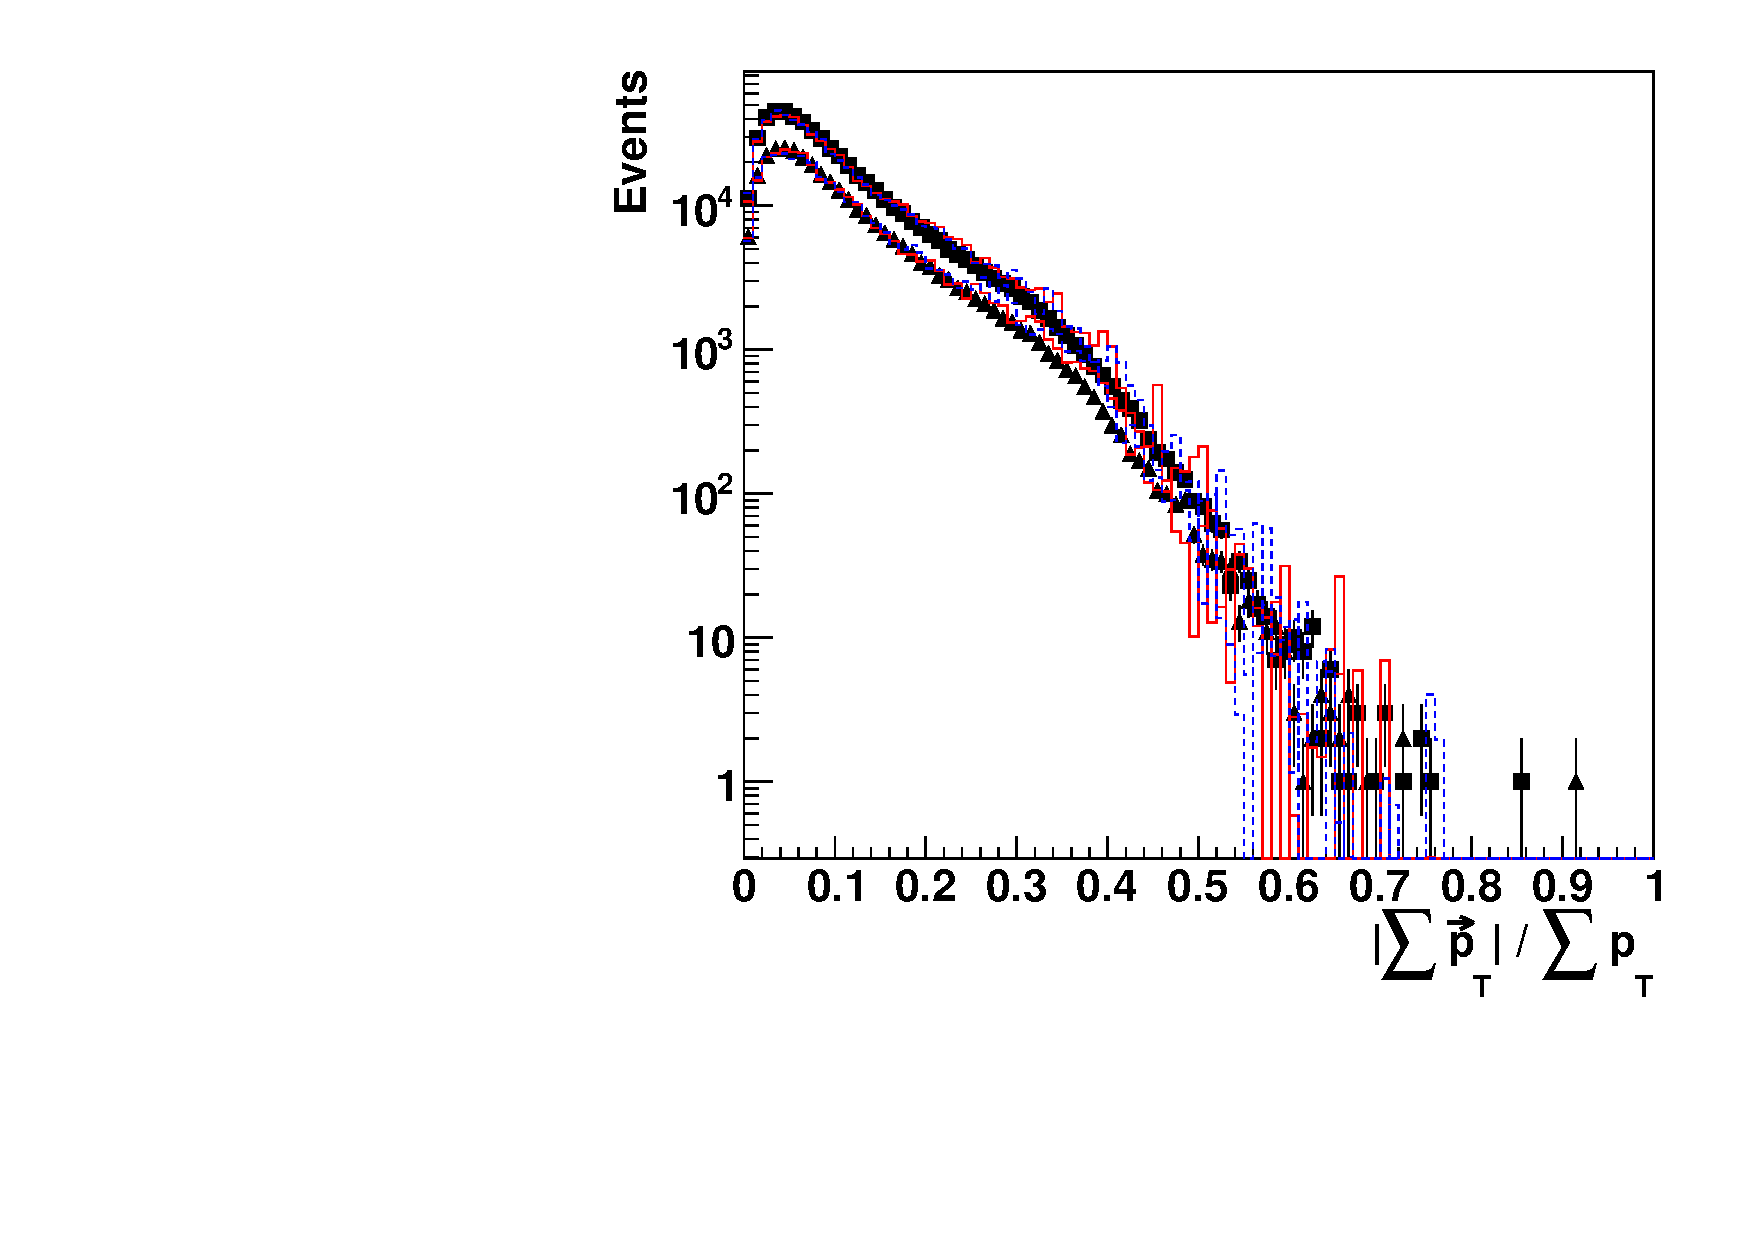
\includegraphics{EXO-12-024/figs/Data-MC-comparisons/PTVSPT-qVMiumHigh.pdf}} \\
%\end{tabular}
%  \caption[Delta Eta Single]{Comparisons between data and Monte Carlo
%                    for $|\sum{\vec{p}_{T}}| / \sum{p_{T}}$ of the two leading jets of low purity (left) and low-high purity (right) 1-tagged events.
%	   The MC is normalized to the number of data events in each category. }
%  \label{fig:metSumPtSingle}
%\end{figure}

%\begin{figure}[htb]
%\centering
%\begin{tabular}{cc}
%     \resizebox{0.5\linewidth}{!}{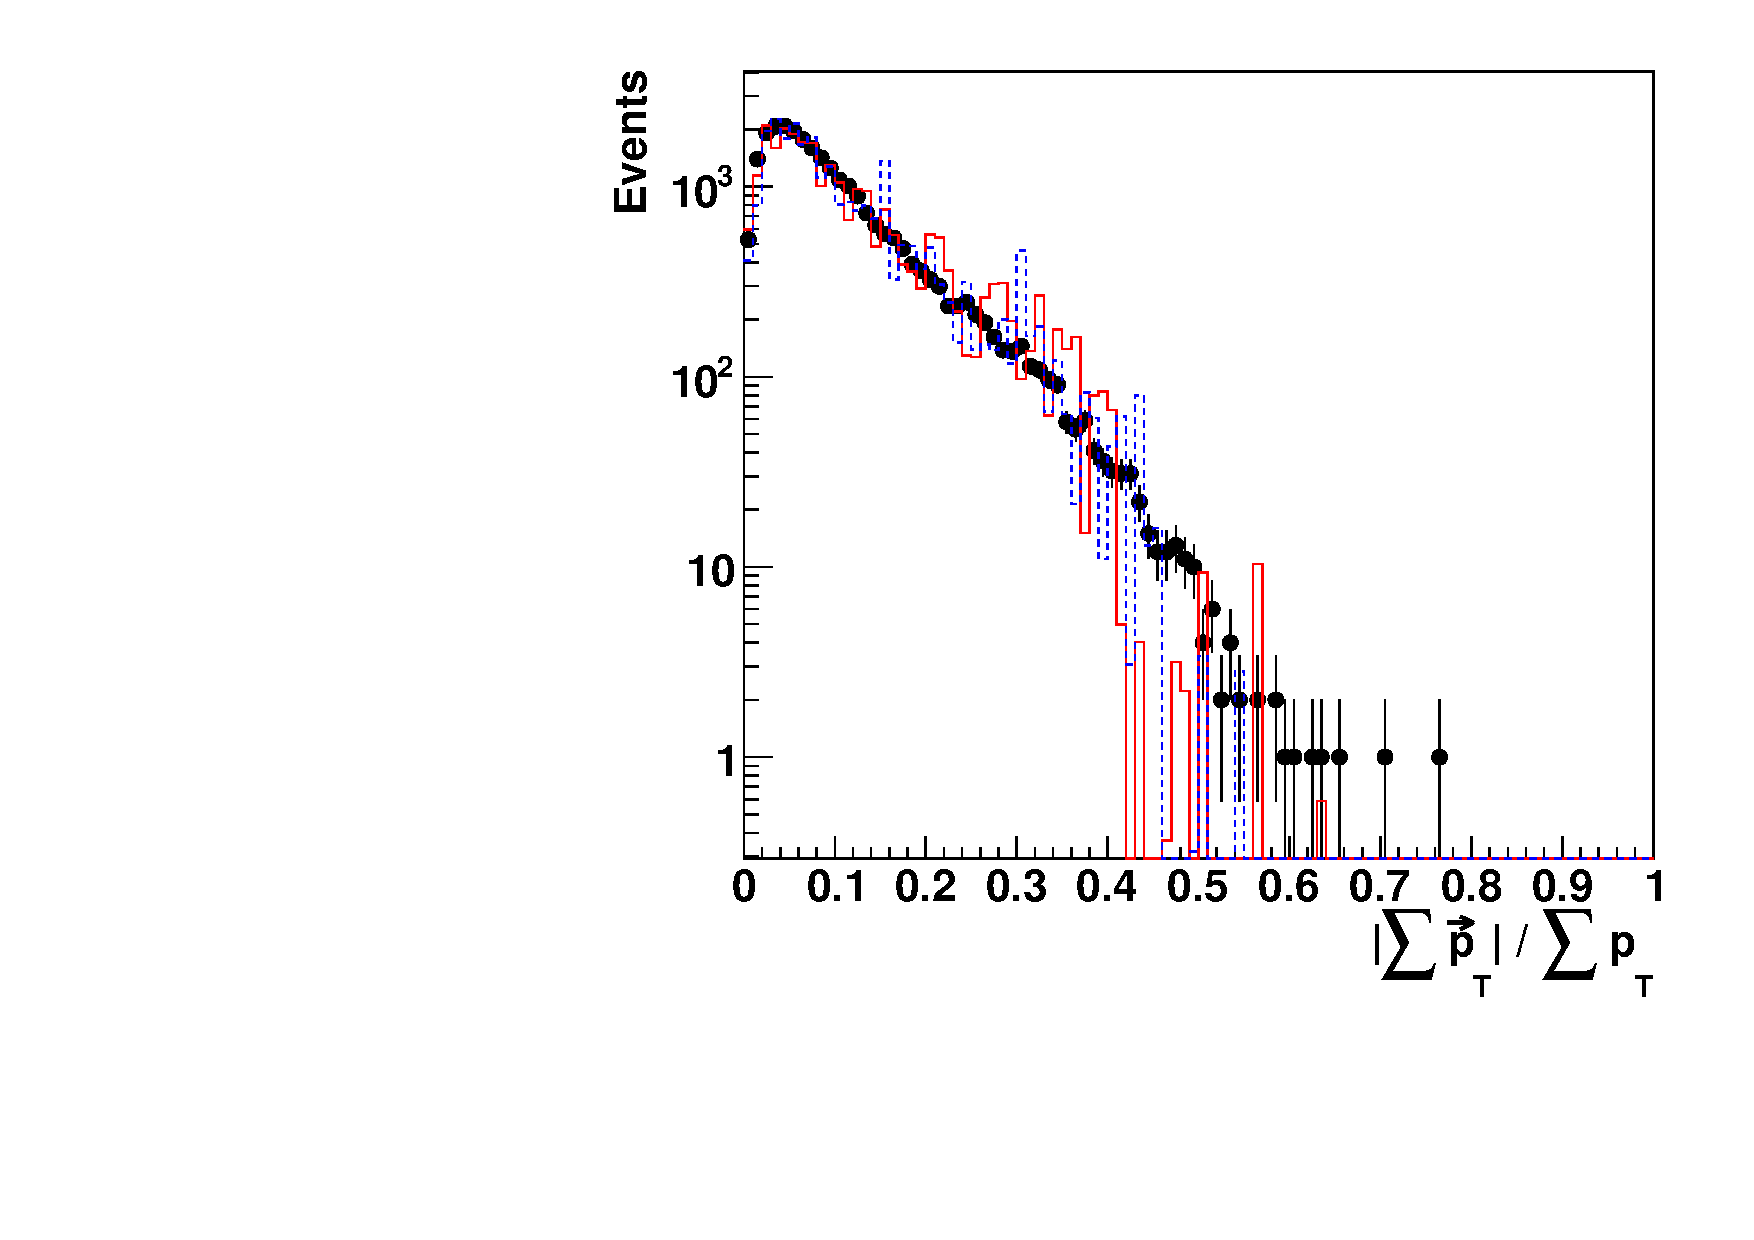
\includegraphics{EXO-12-024/figs/Data-MC-comparisons/PTVSPT-VVLowP.pdf}} &
%     \resizebox{0.5\linewidth}{!}{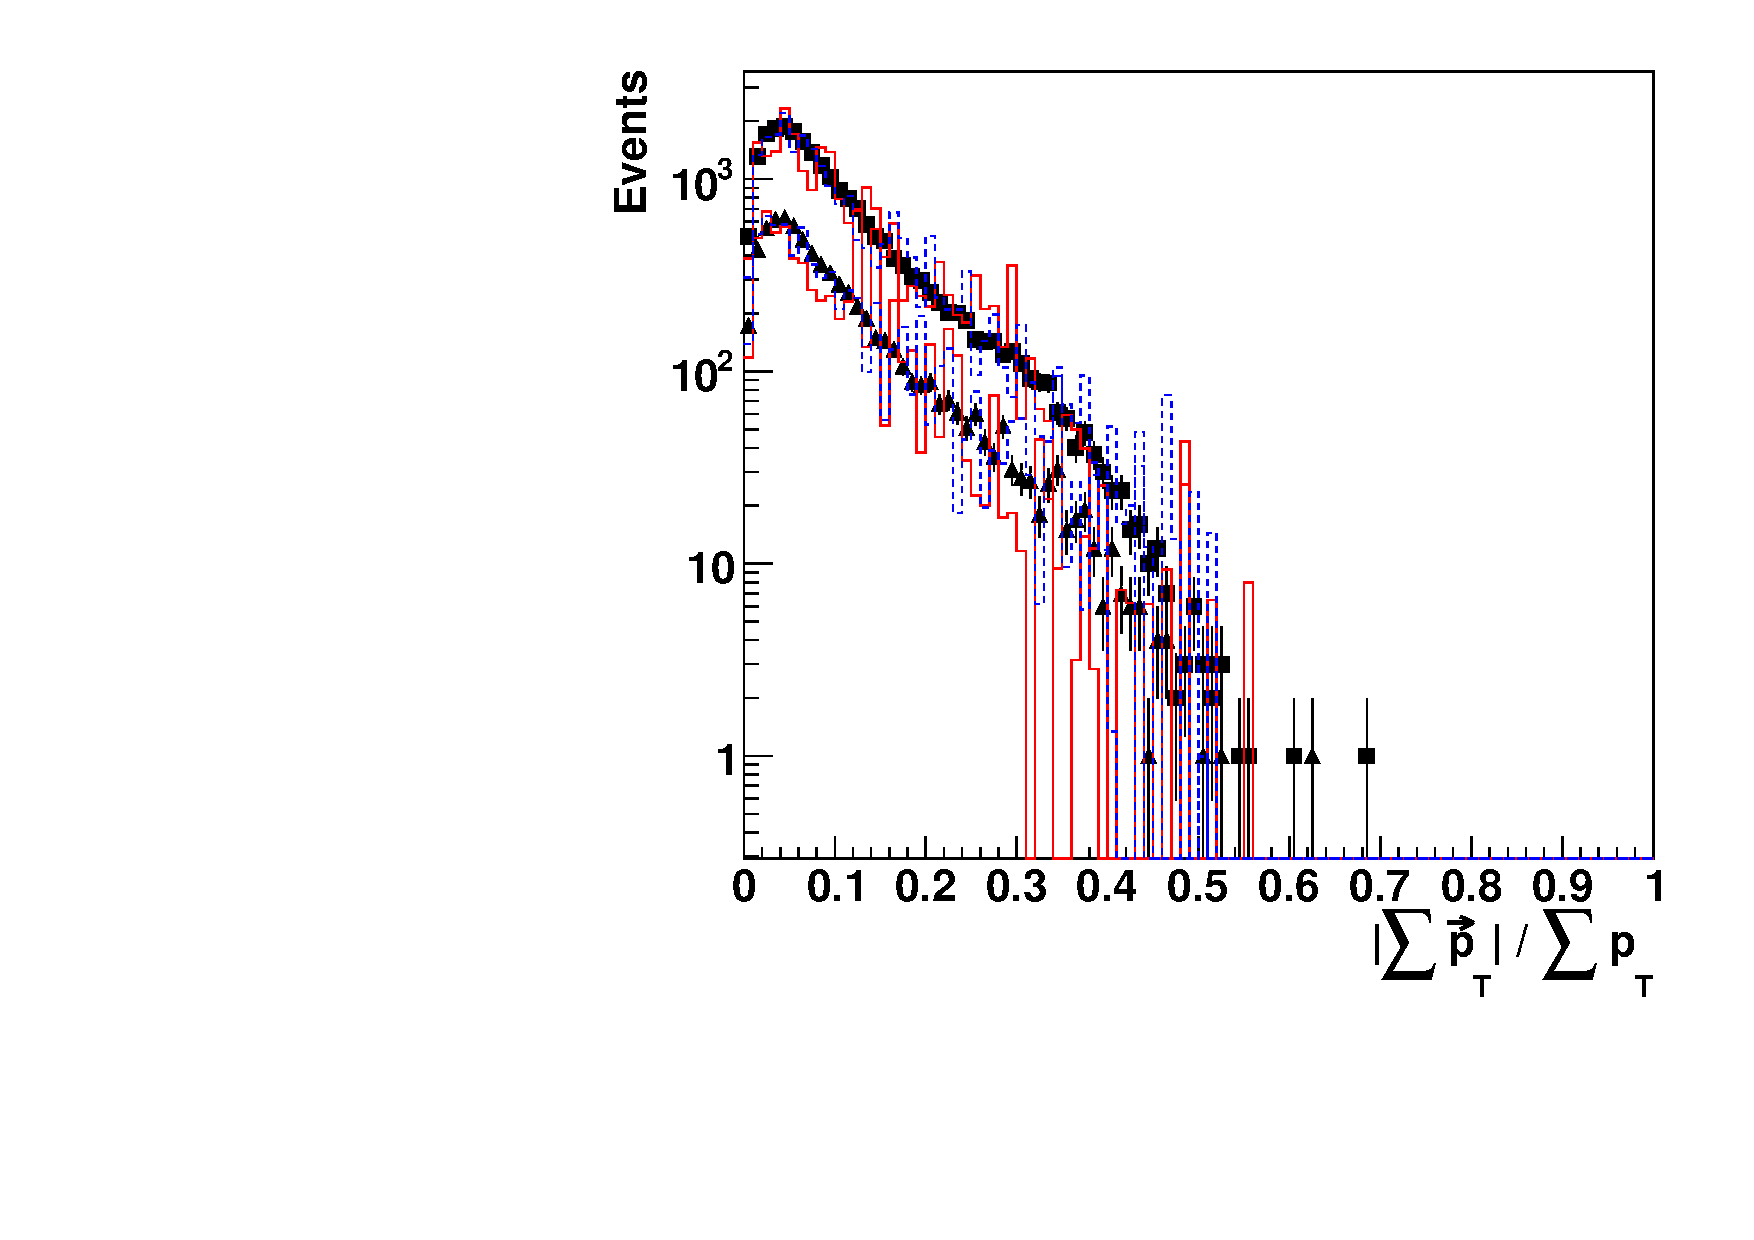
\includegraphics{EXO-12-024/figs/Data-MC-comparisons/PTVSPT-VVMiumHigh.pdf}} \\
%\end{tabular}
%  \caption[Delta Eta Double]{Comparisons between data and Monte Carlo
%                     for $|\sum{\vec{p}_{T}}| / \sum{p_{T}}$ of the two leading jets of low purity (left) and low-high purity (right) 2-tagged events. The MC is normalized to the number of data events in each category. }
%  \label{fig:metSumPtDouble}
%\end{figure}

\newpage
\begin{figure}[htb]
\centering
\begin{tabular}{cc}
     \resizebox{0.5\linewidth}{!}{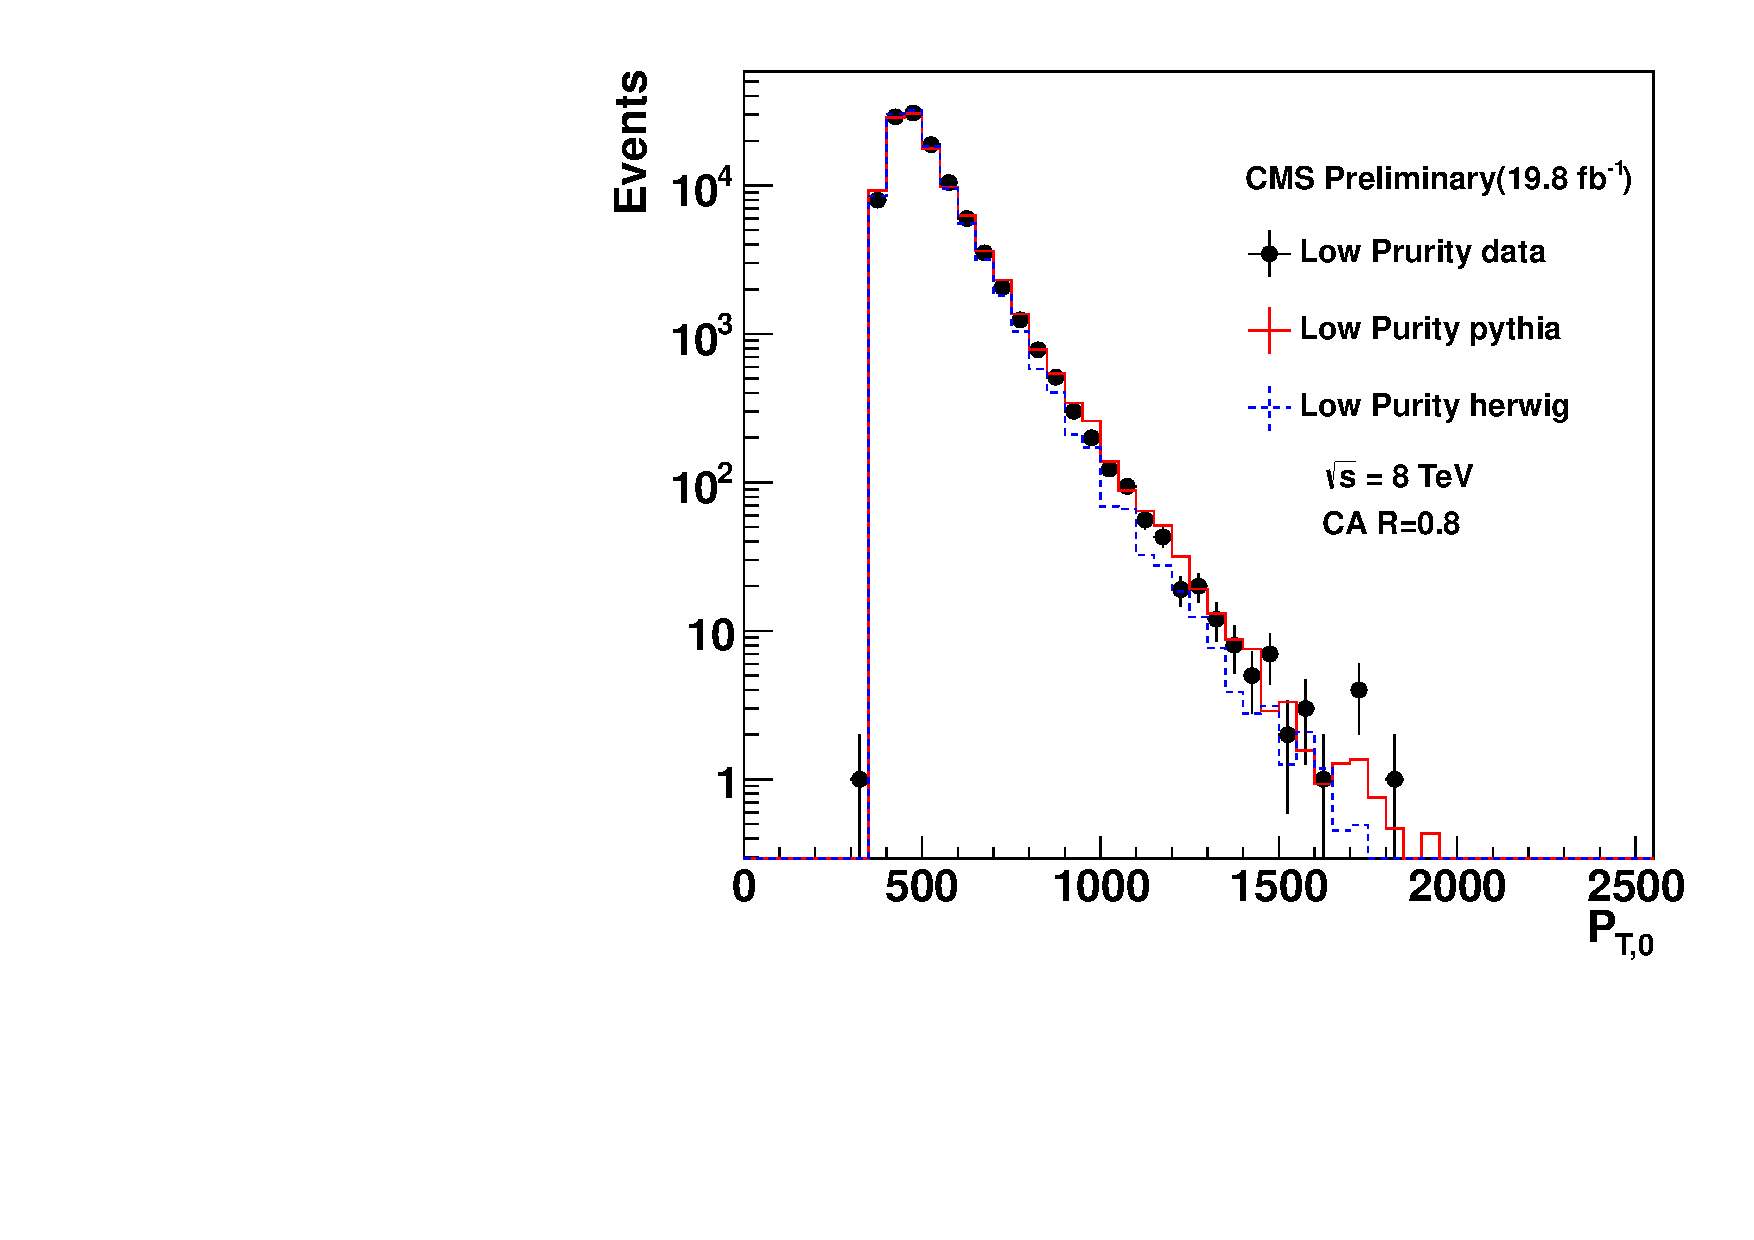
\includegraphics{EXO-12-024/figs/Data-MC-comparisons/PT0-qVLowP.pdf}} &
     \resizebox{0.5\linewidth}{!}{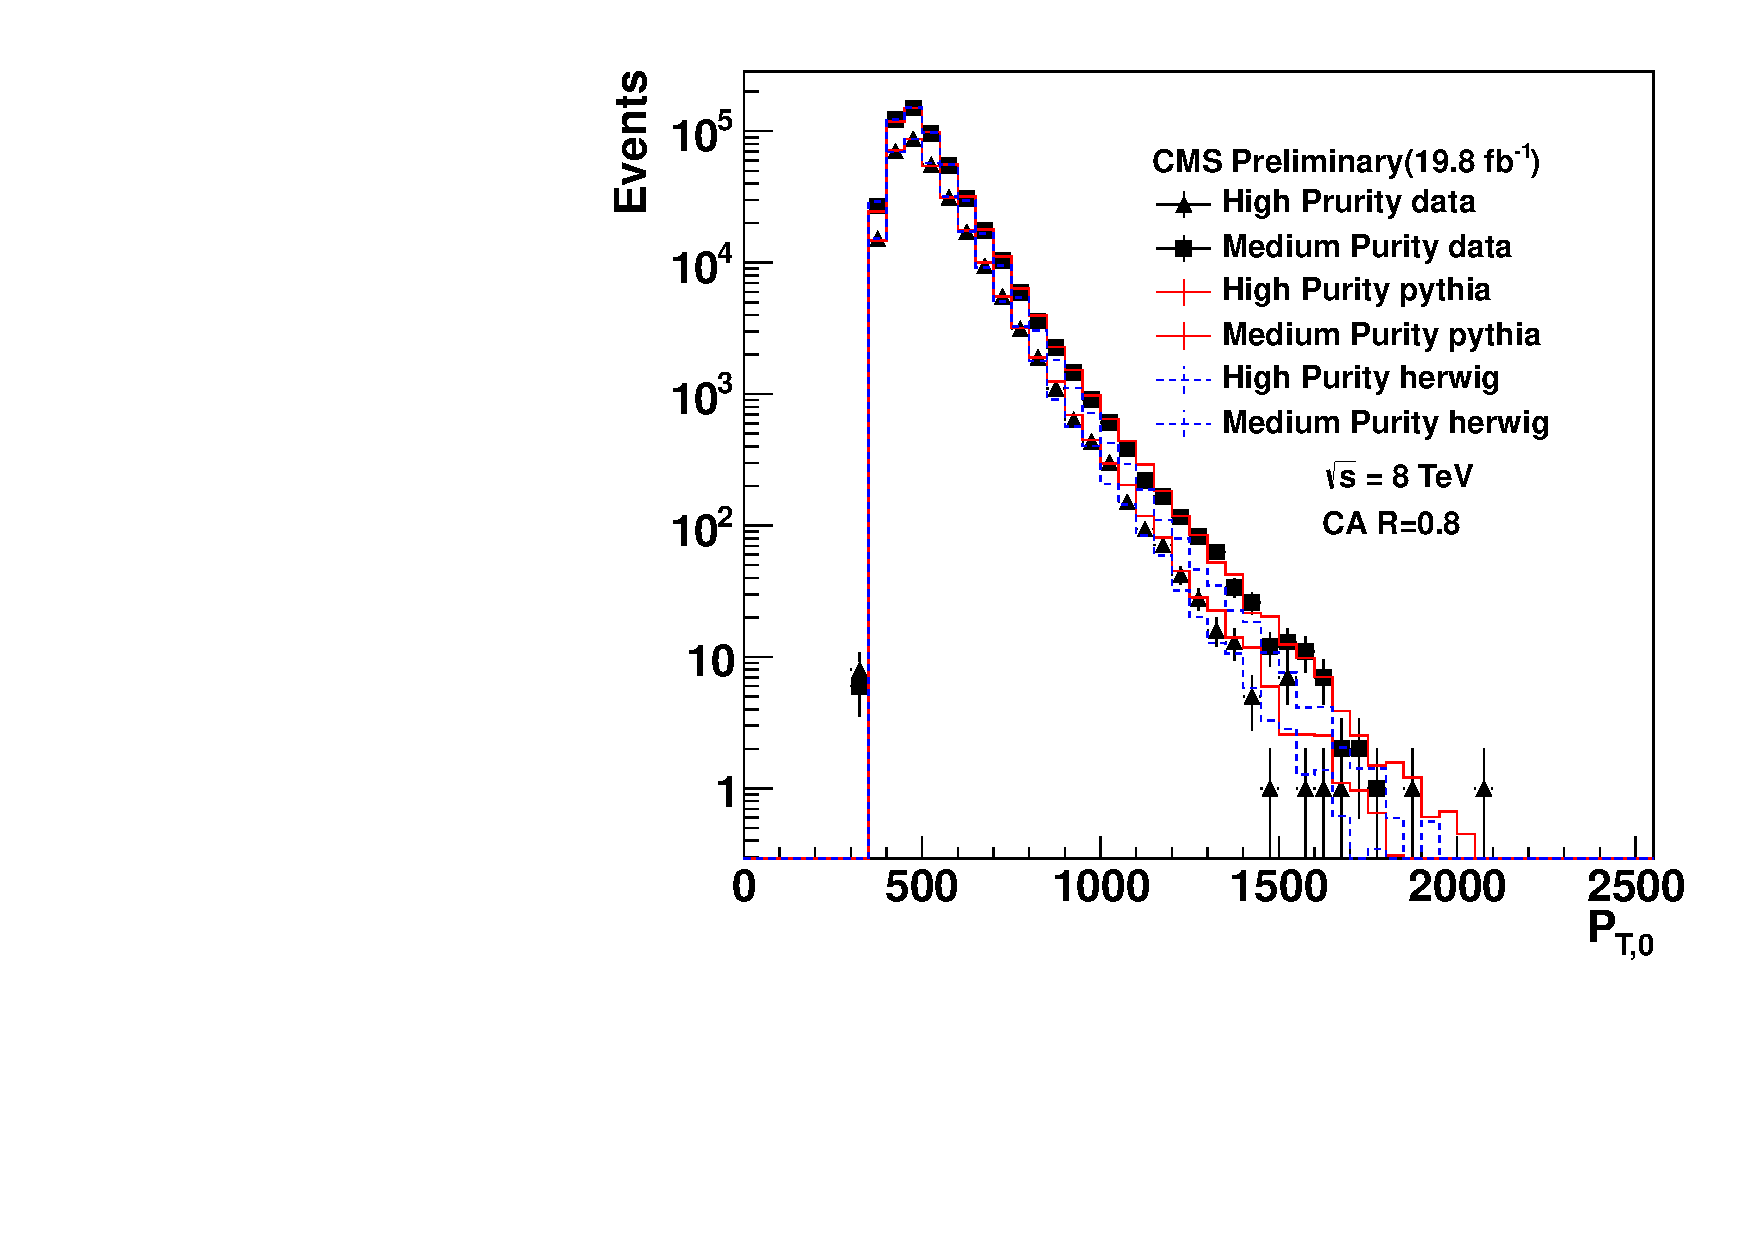
\includegraphics{EXO-12-024/figs/Data-MC-comparisons/PT0-qVMiumHigh.pdf}} \\
\end{tabular}
  \caption[PT Single]{Comparisons between data and Monte Carlo
                    for $\pt$ of the leading jet of low purity (left) and low-high purity (right) 1-tagged events.
	   The MC is normalized to the number of data events in each category. }
  \label{fig:Pt0Single}
\end{figure}

\begin{figure}[htb]
\centering
\begin{tabular}{cc}
     \resizebox{0.5\linewidth}{!}{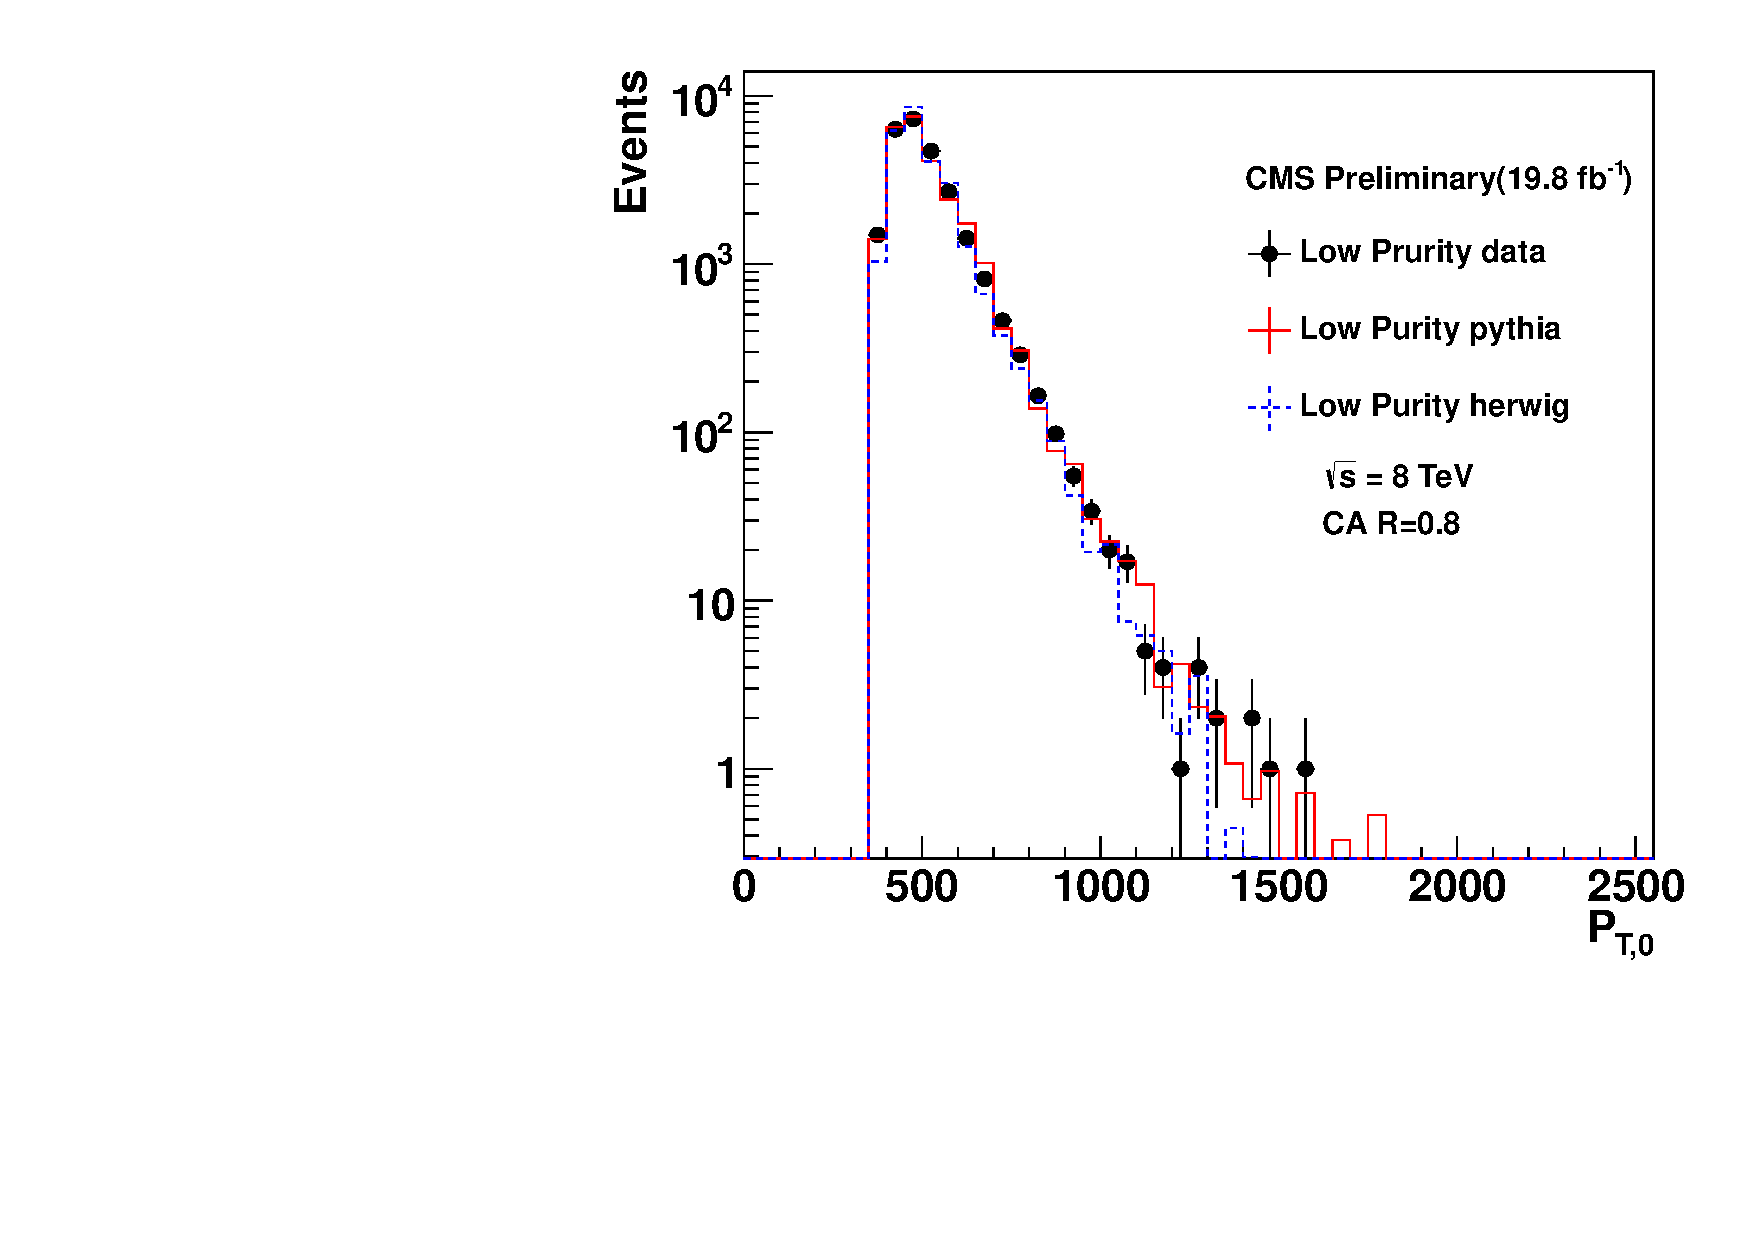
\includegraphics{EXO-12-024/figs/Data-MC-comparisons/PT0-VVLowP.pdf}} &
     \resizebox{0.5\linewidth}{!}{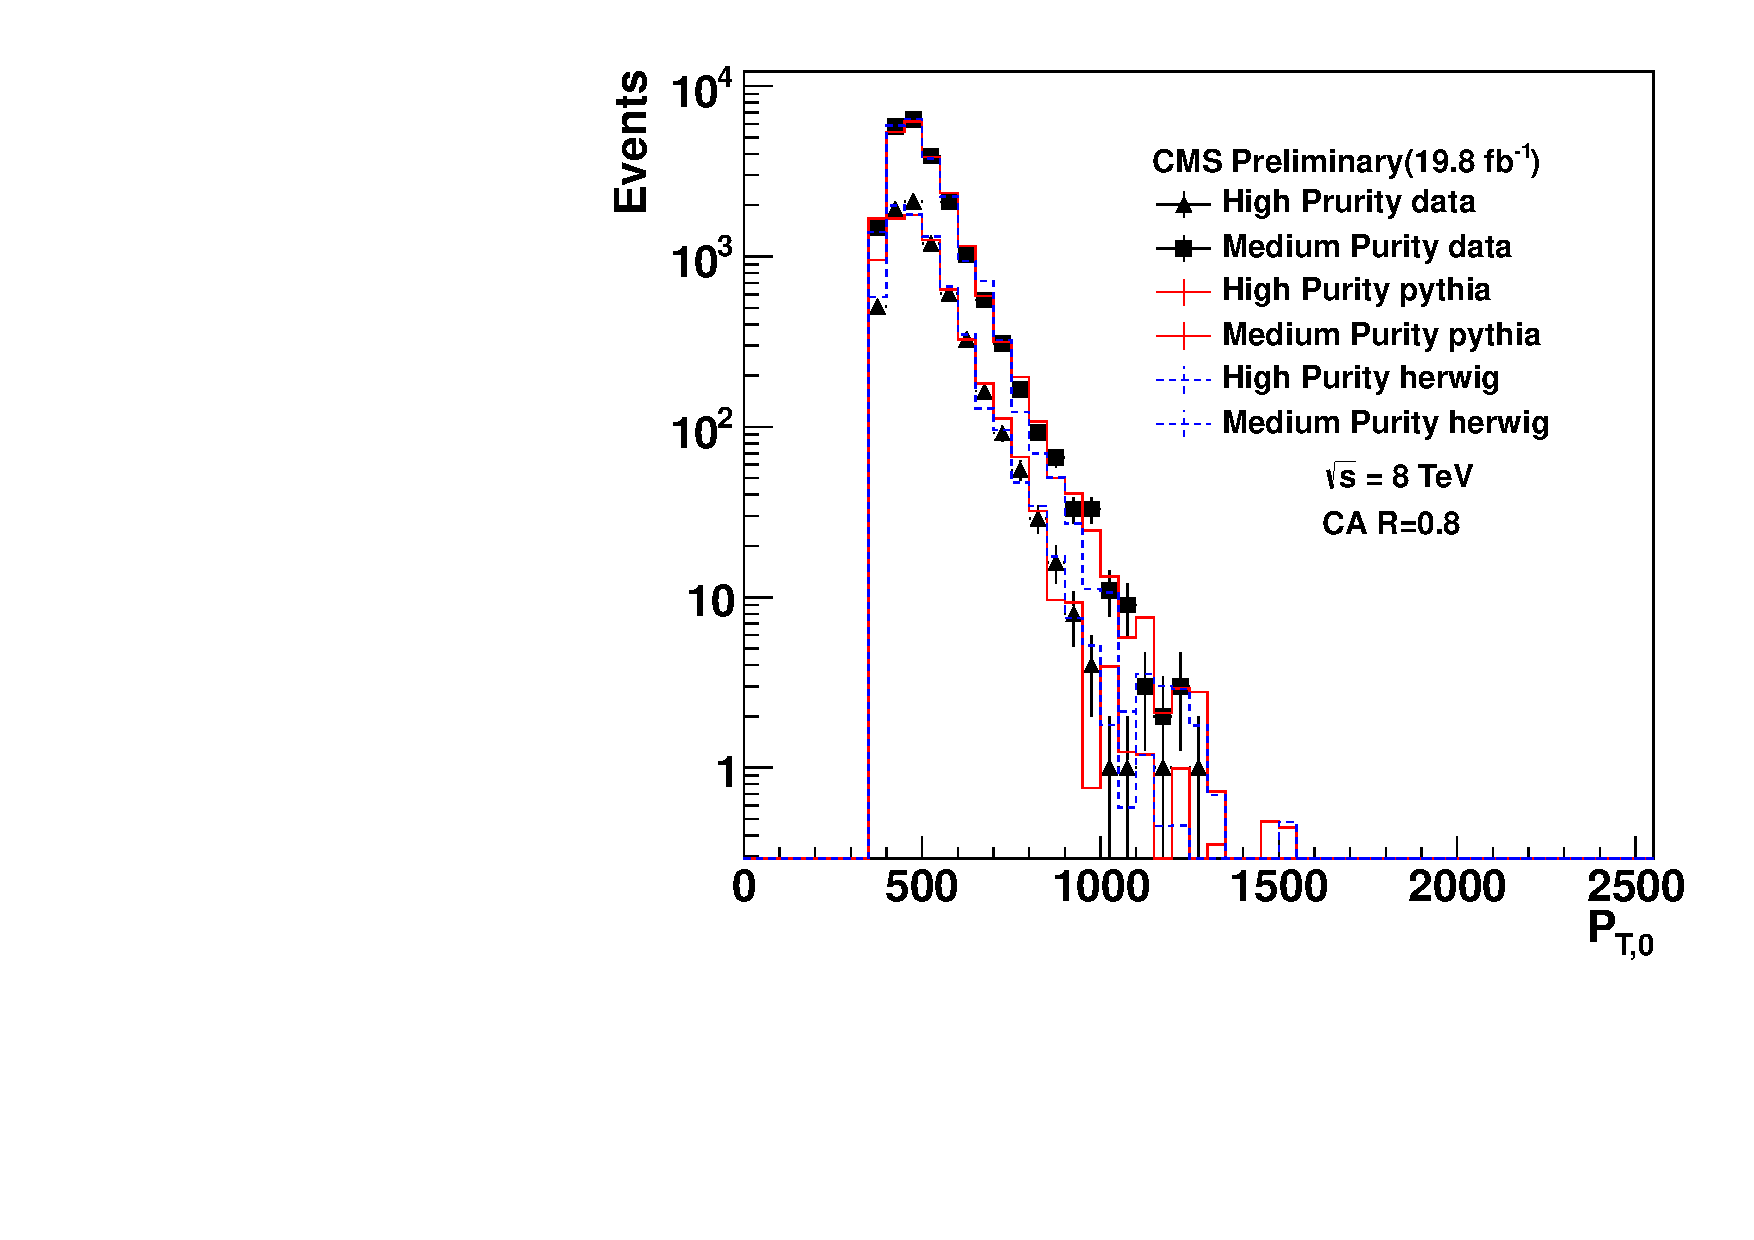
\includegraphics{EXO-12-024/figs/Data-MC-comparisons/PT0-VVMiumHigh.pdf}} \\
\end{tabular}
  \caption[Delta Eta Double]{Comparisons between data and Monte Carlo
                     for $\pt$ of the leading jet of low purity (left) and low-high purity (right) 2-tagged events. The MC is normalized to the number of data events in each category. }
  \label{fig:Pt0Double}
\end{figure}

\newpage
\begin{figure}[htb]
\centering
\begin{tabular}{cc}
     \resizebox{0.5\linewidth}{!}{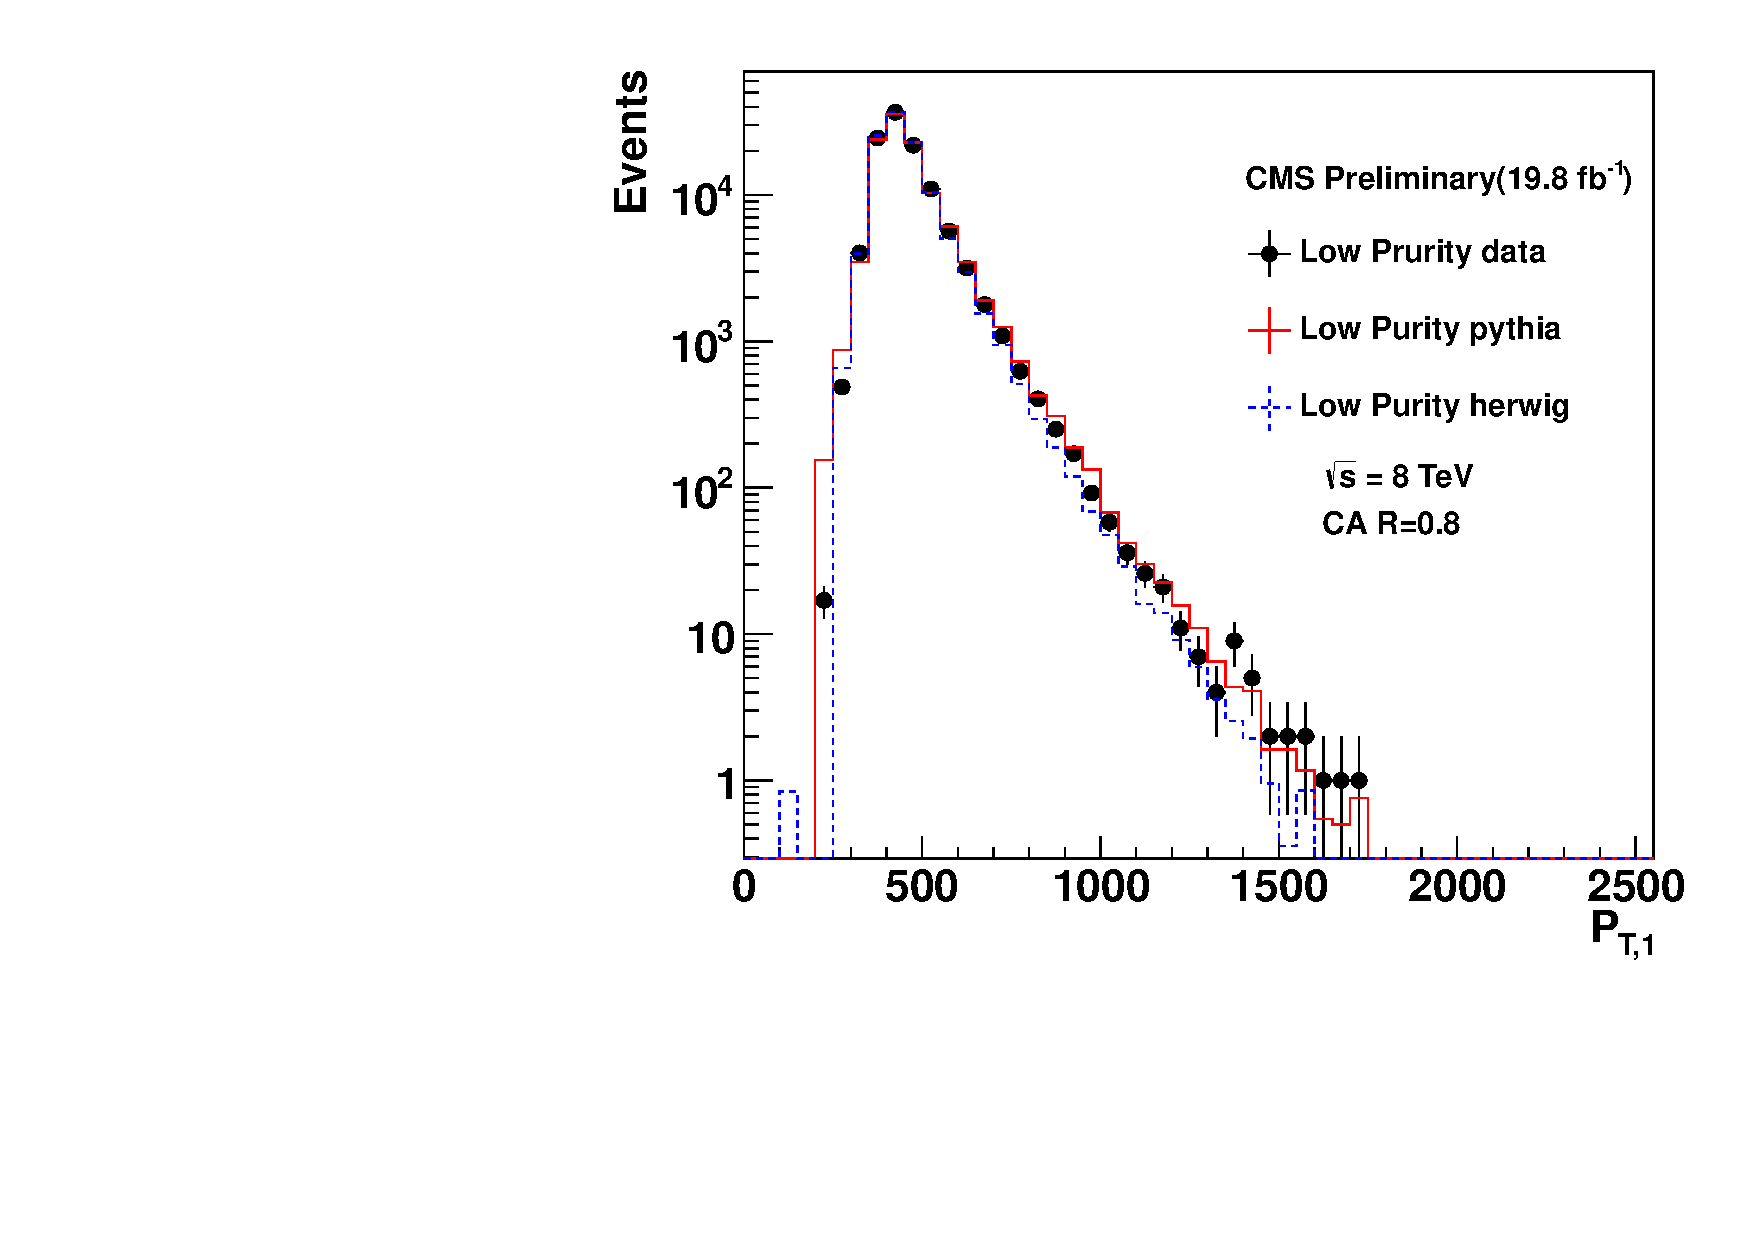
\includegraphics{EXO-12-024/figs/Data-MC-comparisons/PT1-qVLowP.pdf}} &
     \resizebox{0.5\linewidth}{!}{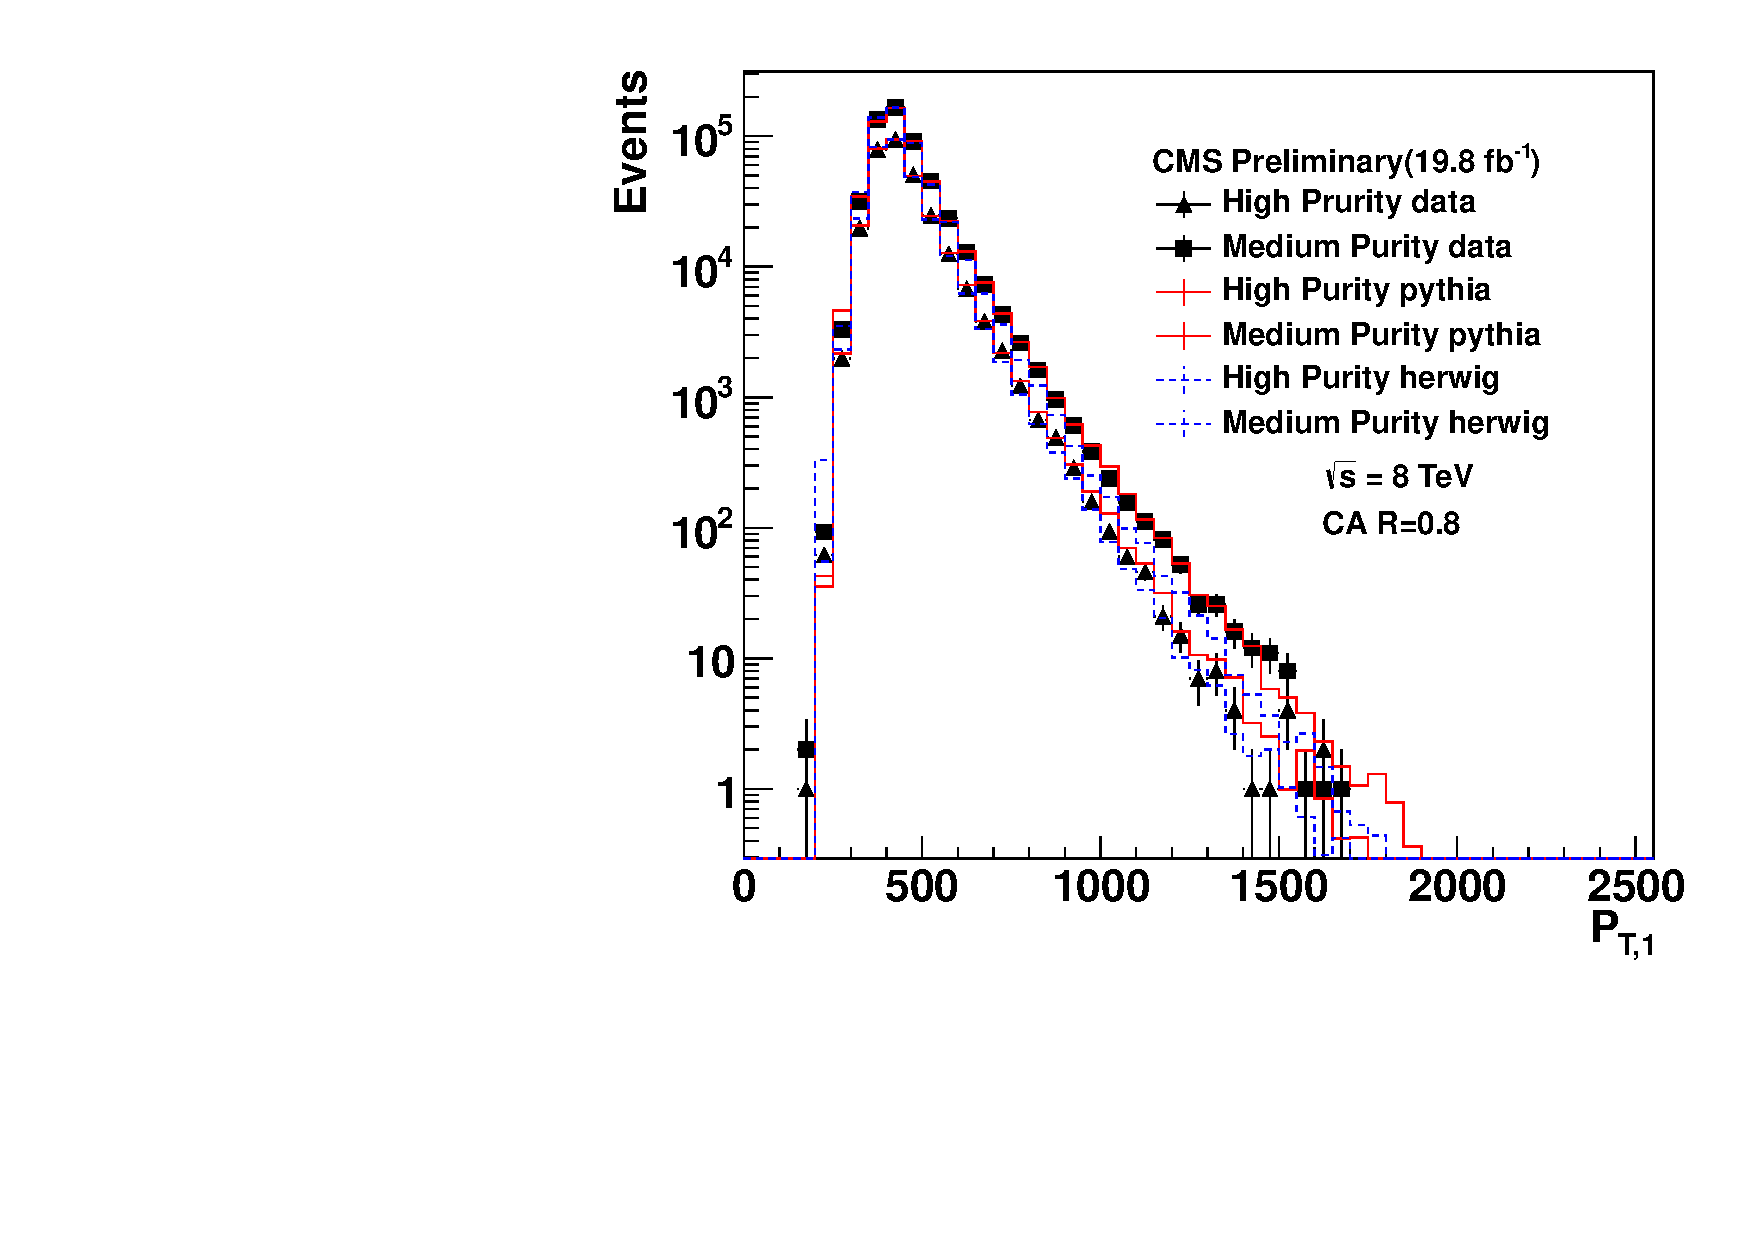
\includegraphics{EXO-12-024/figs/Data-MC-comparisons/PT1-qVMiumHigh.pdf}} \\
\end{tabular}
  \caption[PT Single]{Comparisons between data and Monte Carlo
                    for $\pt$ of the second leading jet of low purity (left) and low-high purity (right) 1-tagged events.
	   The MC is normalized to the number of data events in each category. }
  \label{fig:Pt1Single}
\end{figure}

\begin{figure}[htb]
\centering
\begin{tabular}{cc}
     \resizebox{0.5\linewidth}{!}{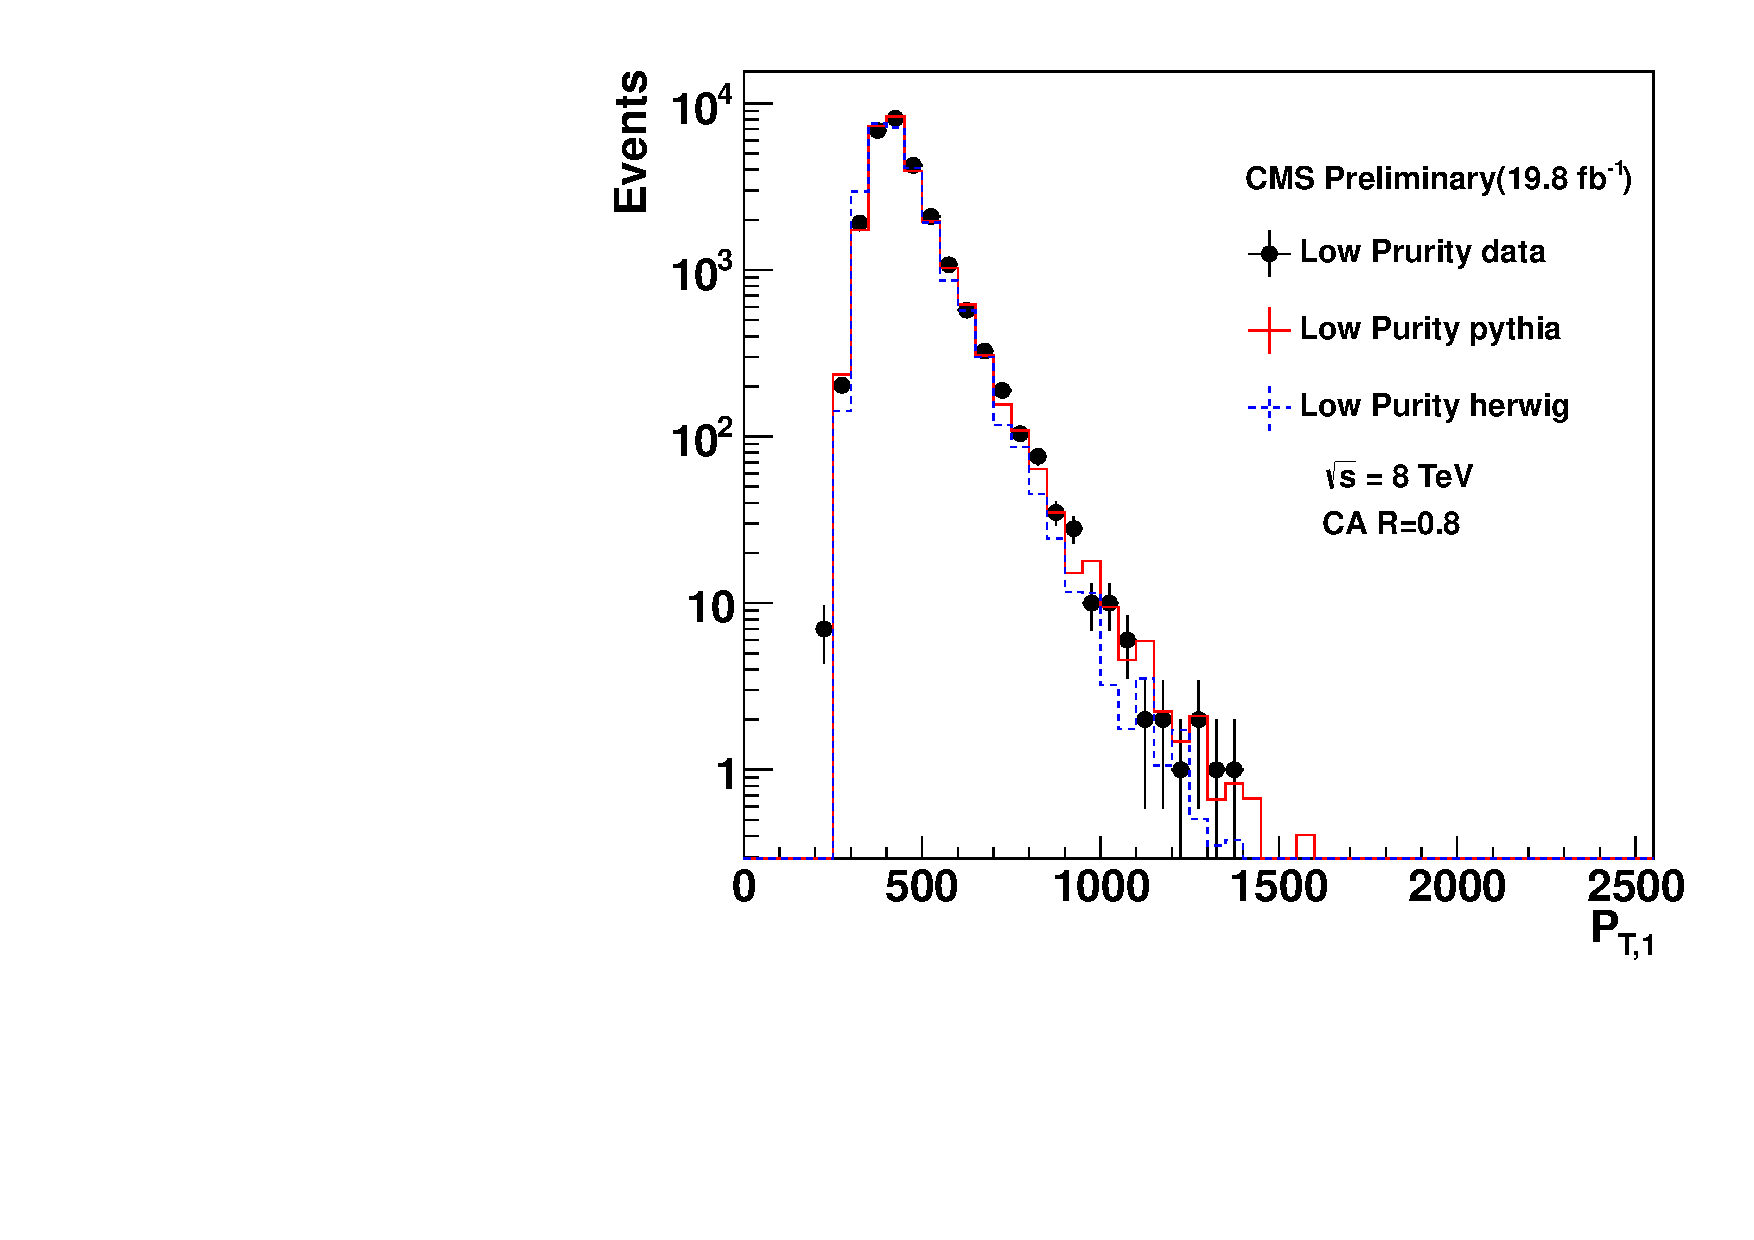
\includegraphics{EXO-12-024/figs/Data-MC-comparisons/PT1-VVLowP.pdf}} &
     \resizebox{0.5\linewidth}{!}{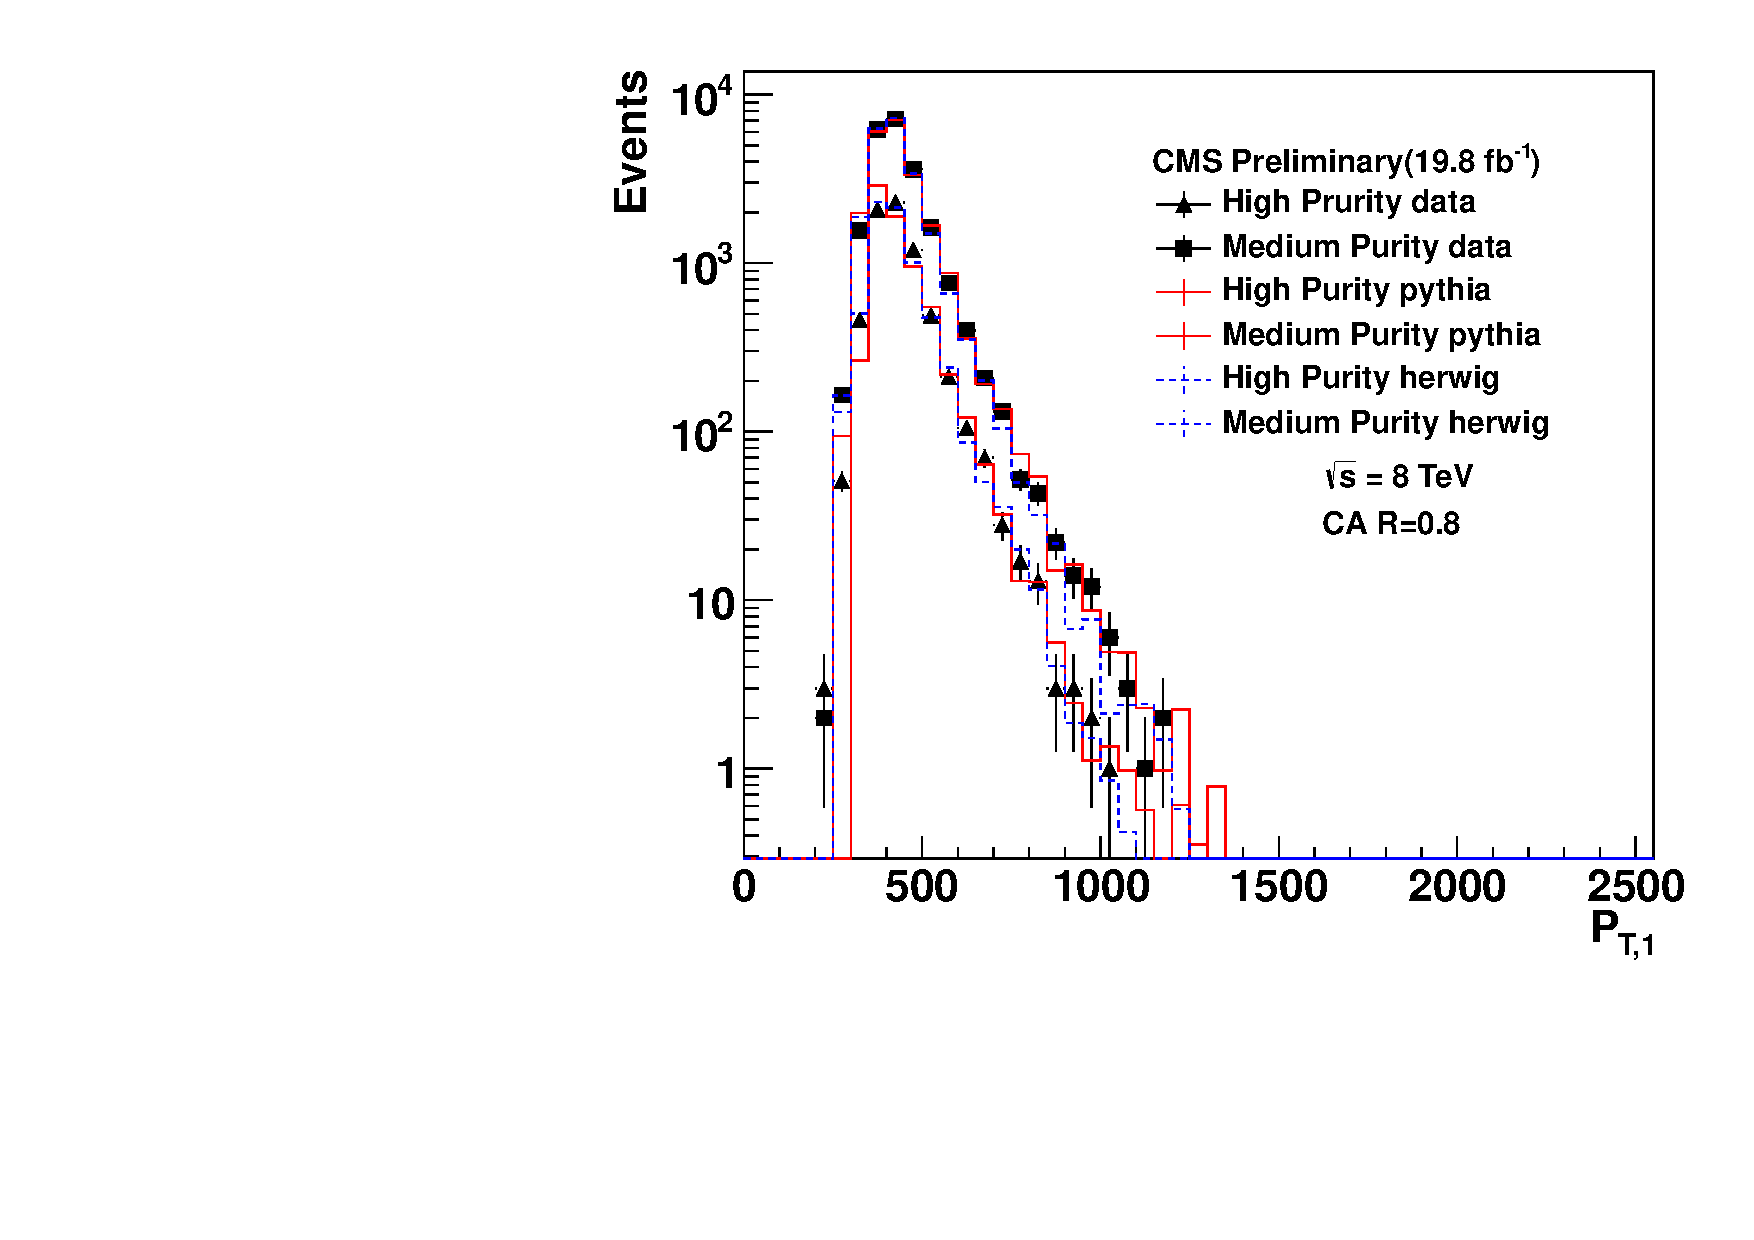
\includegraphics{EXO-12-024/figs/Data-MC-comparisons/PT1-VVMiumHigh.pdf}} \\
\end{tabular}
  \caption[Delta Eta Double]{Comparisons between data and Monte Carlo
                     for $\pt$ of the second leading jet of low purity (left) and low-high purity (right) 2-tagged events. The MC is normalized to the number of data events in each category. }
  \label{fig:Pt1Double}
\end{figure}



\newpage
\begin{figure}[htb]
\centering
\begin{tabular}{cc}
     \resizebox{0.5\linewidth}{!}{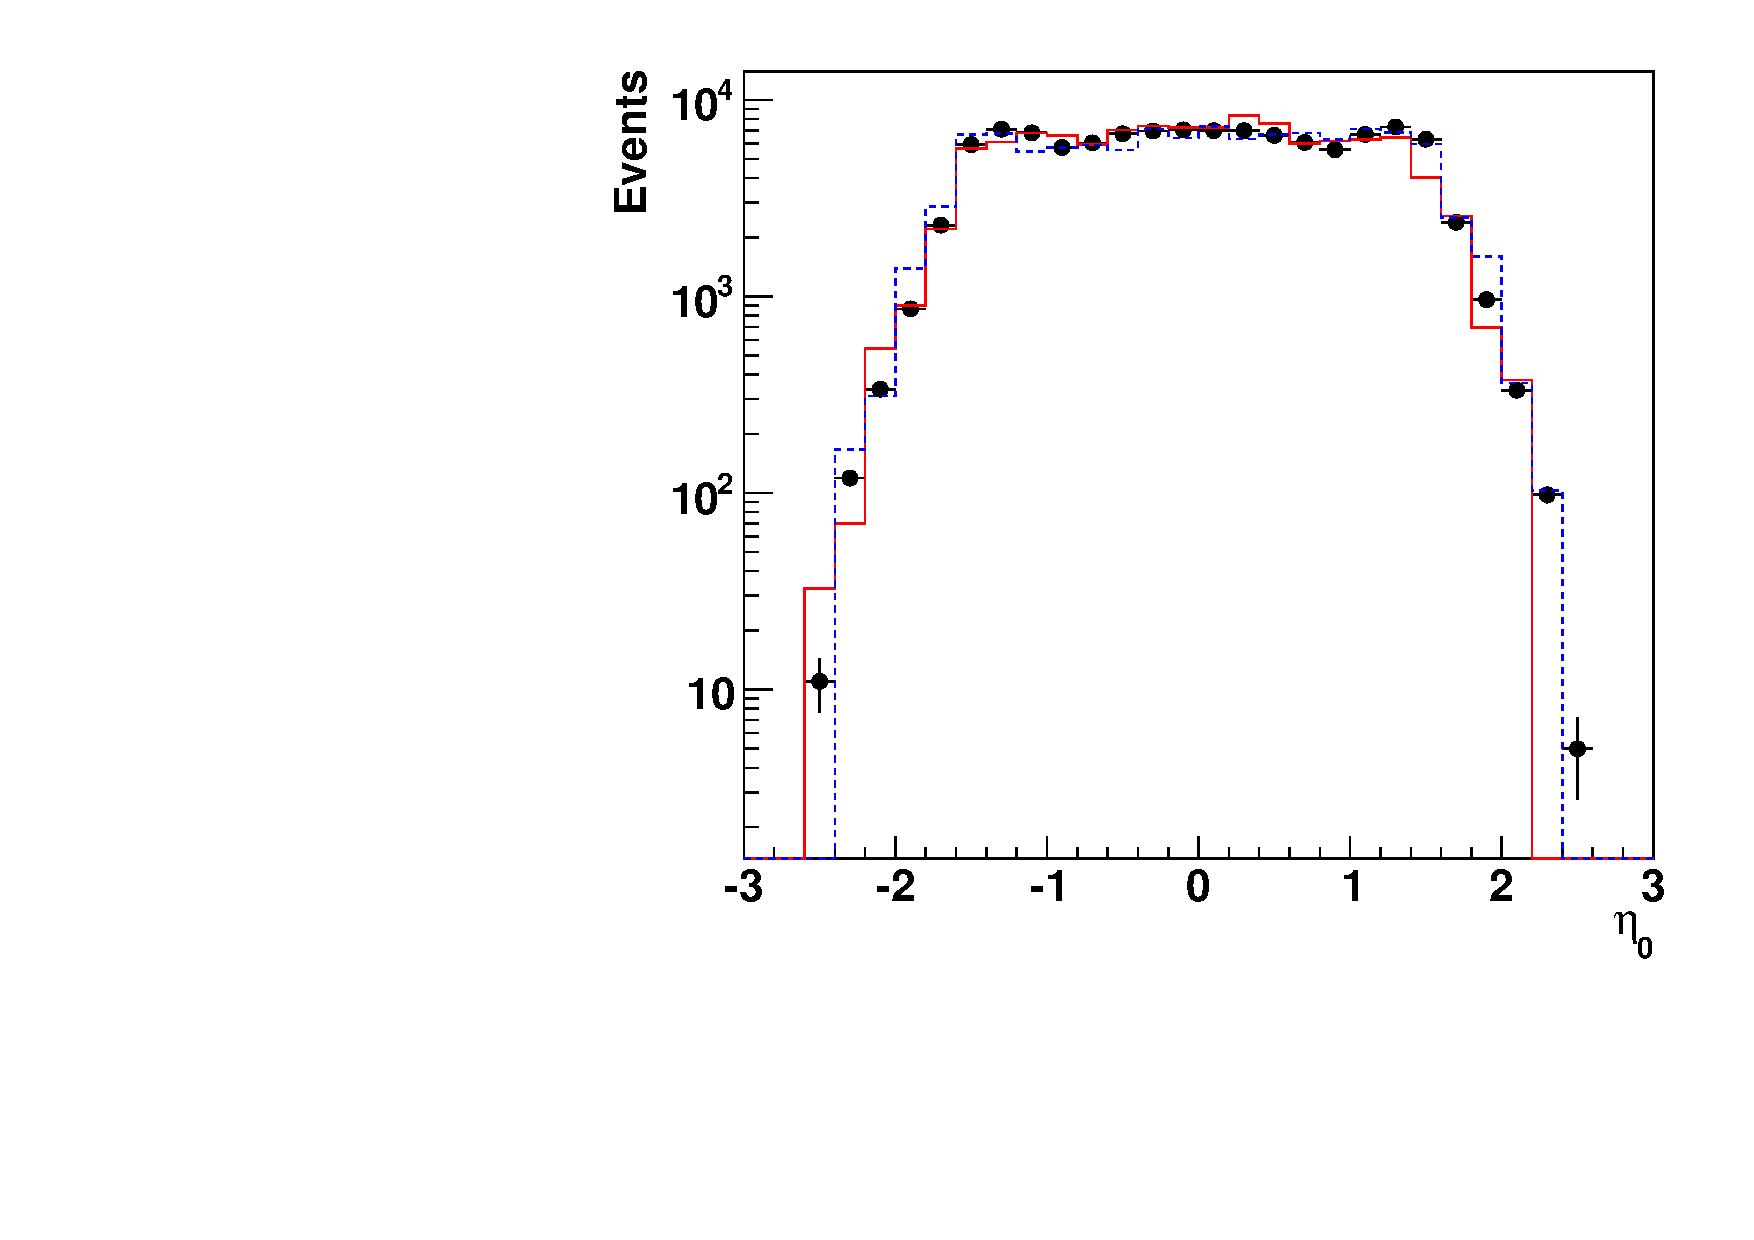
\includegraphics{EXO-12-024/figs/Data-MC-comparisons/Eta0-qVLowP.pdf}} &
     \resizebox{0.5\linewidth}{!}{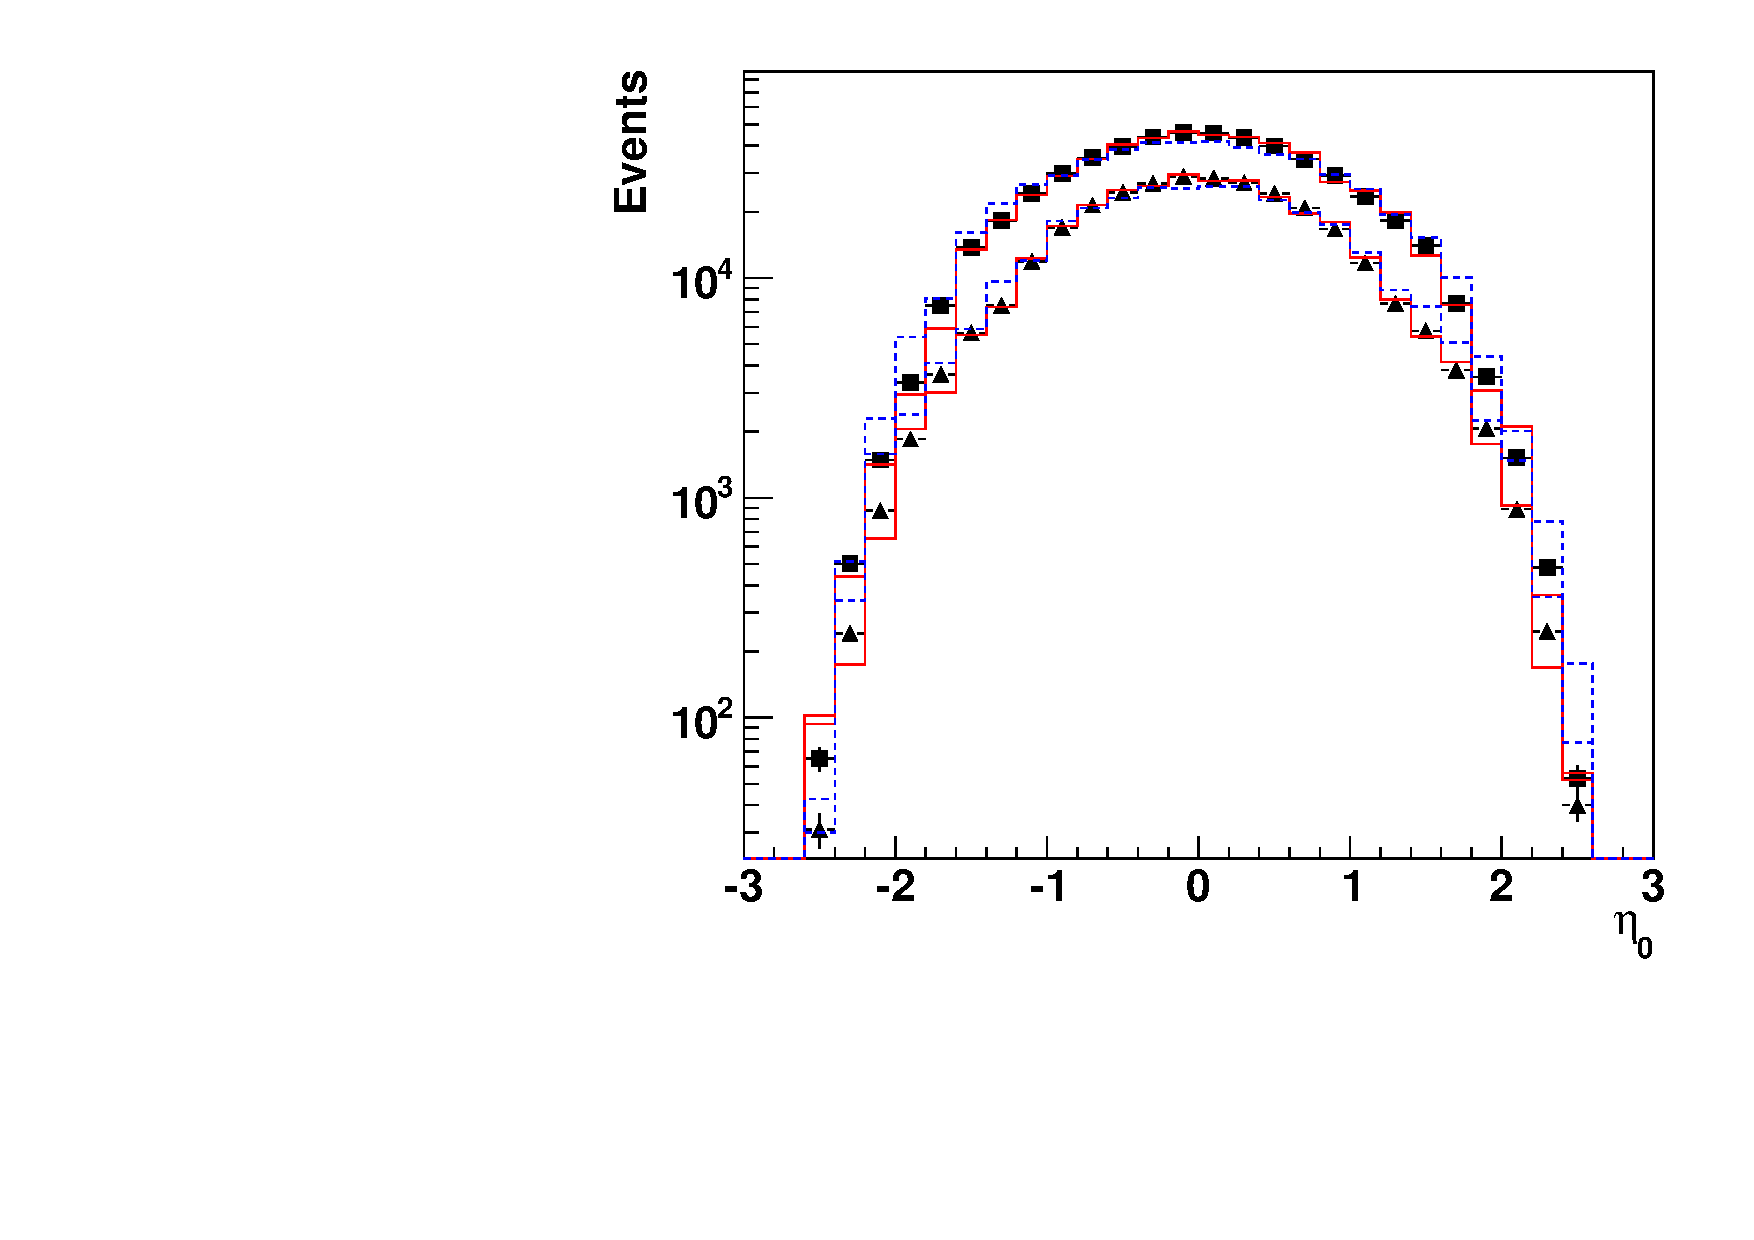
\includegraphics{EXO-12-024/figs/Data-MC-comparisons/Eta0-qVMiumHigh.pdf}} \\
\end{tabular}
  \caption[PT Single]{Comparisons between data and Monte Carlo
                    for $\eta$ of the leading jet of low purity (left) and low-high purity (right) 1-tagged events.
	   The MC is normalized to the number of data events in each category. }
  \label{fig:Eta0Single}
\end{figure}

\begin{figure}[htb]
\centering
\begin{tabular}{cc}
     \resizebox{0.5\linewidth}{!}{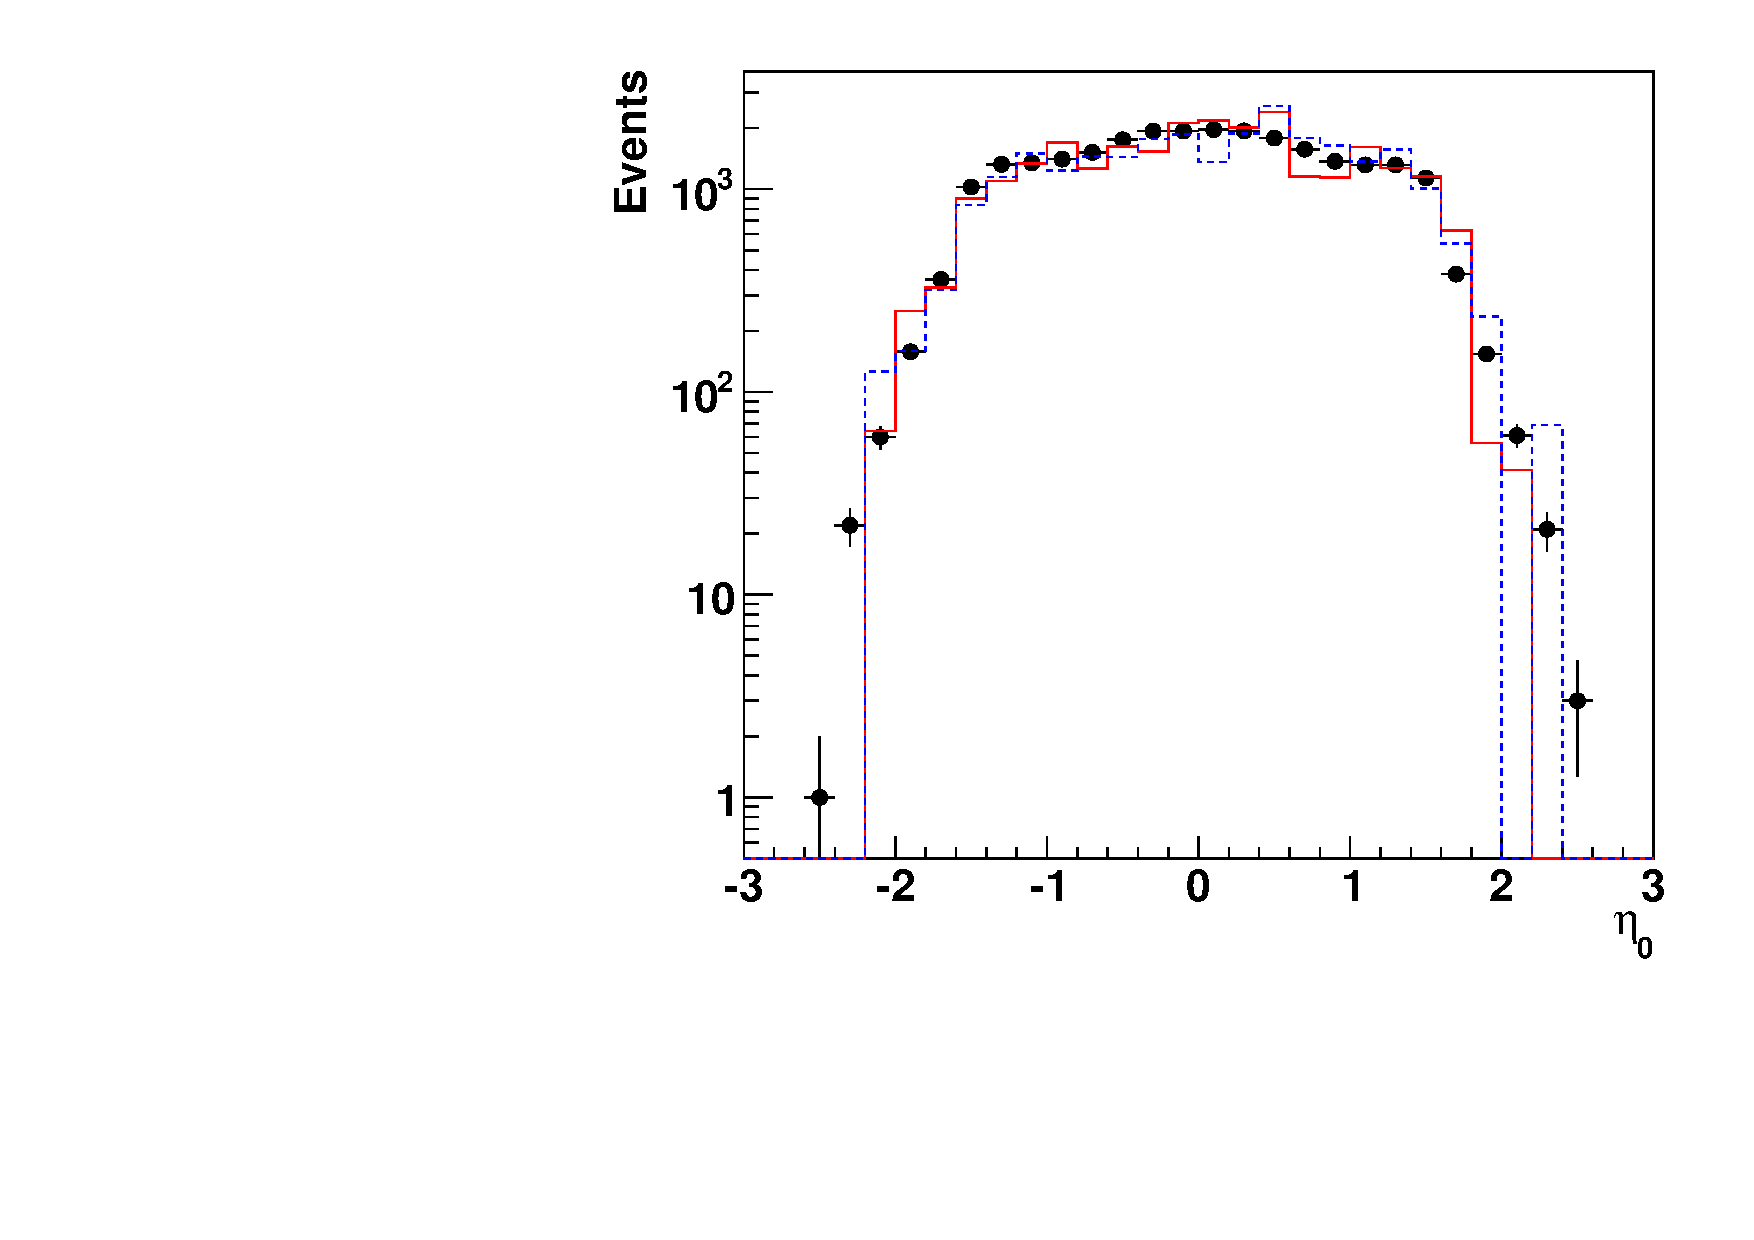
\includegraphics{EXO-12-024/figs/Data-MC-comparisons/Eta0-VVLowP.pdf}} &
     \resizebox{0.5\linewidth}{!}{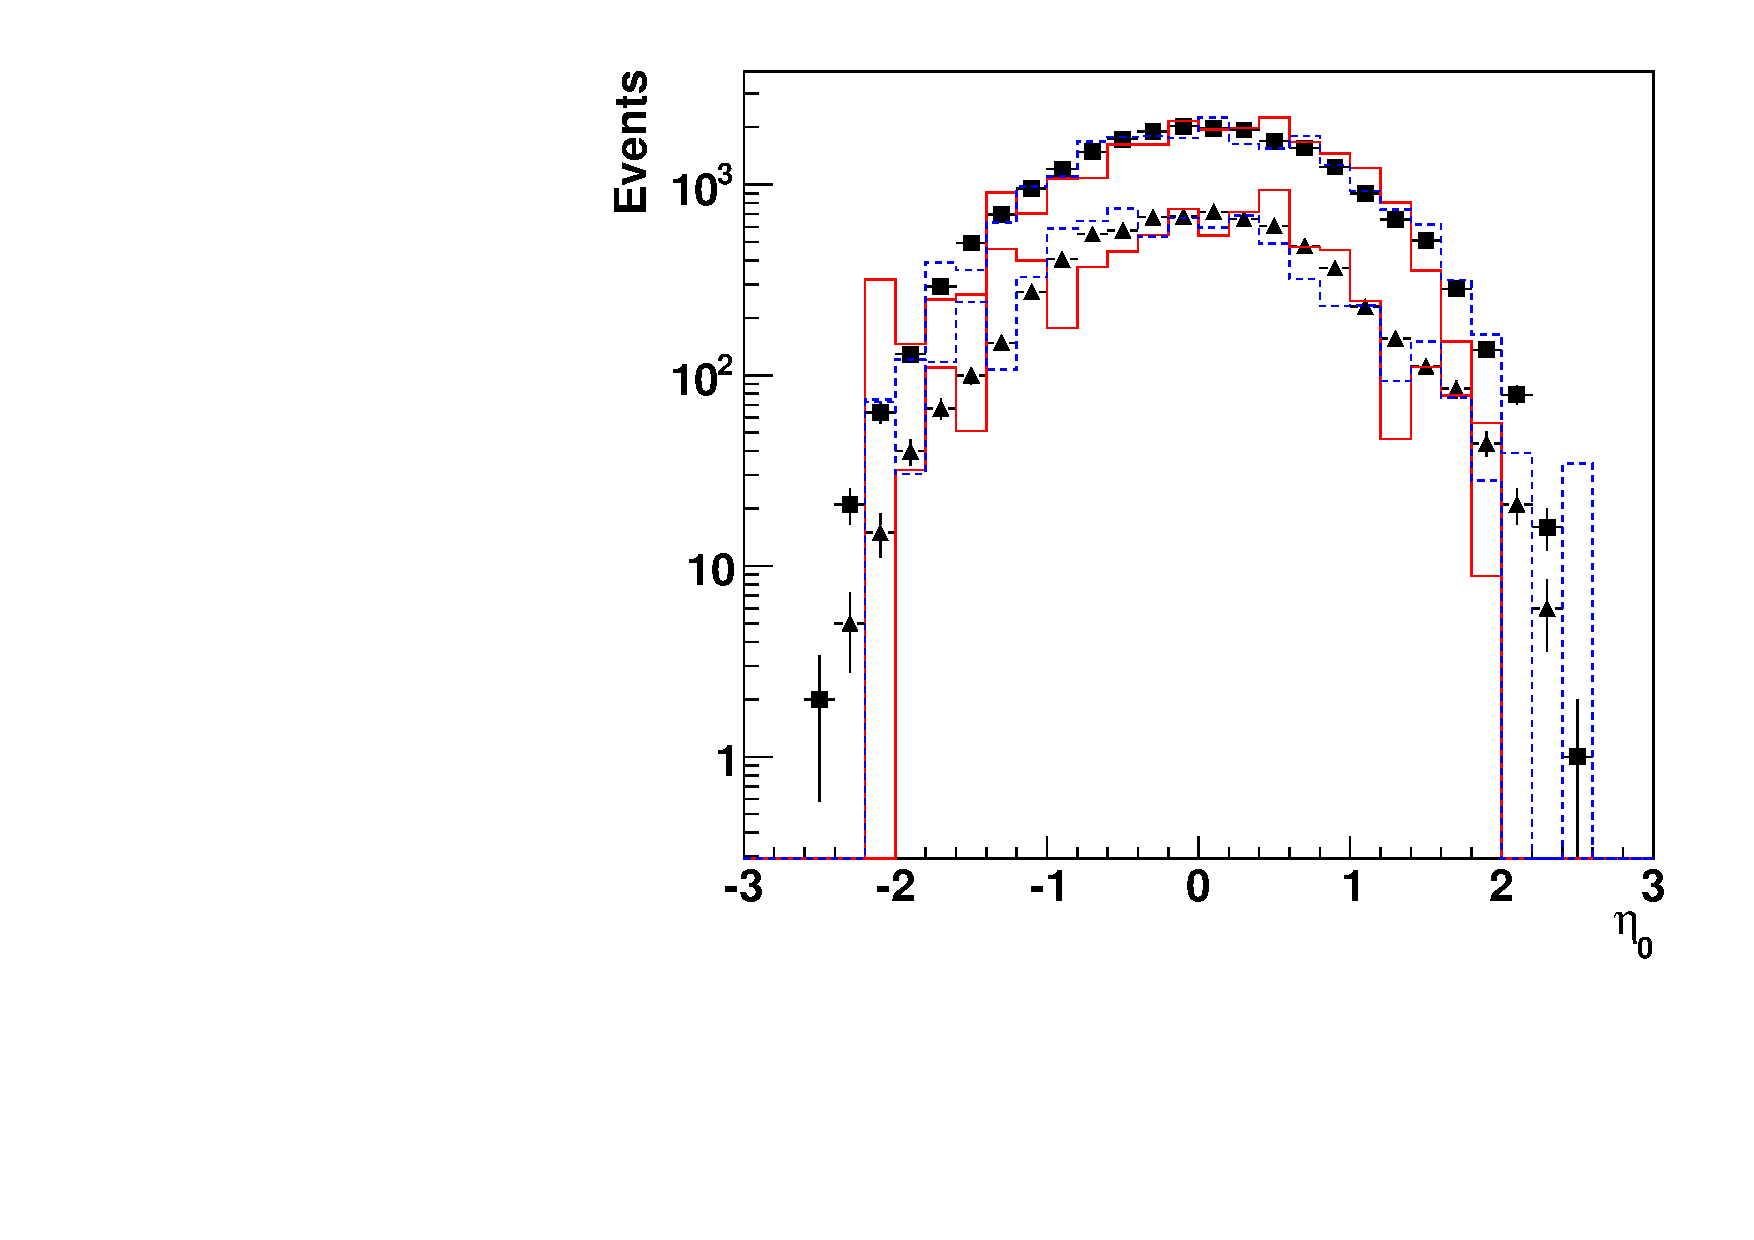
\includegraphics{EXO-12-024/figs/Data-MC-comparisons/Eta0-VVMiumHigh.pdf}} \\
\end{tabular}
  \caption[Delta Eta Double]{Comparisons between data and Monte Carlo
                     for $\eta$ of the leading jet of low purity (left) and low-high purity (right) 2-tagged events. The MC is normalized to the number of data events in each category. }
  \label{fig:Eta0Double}
\end{figure}


\newpage
\begin{figure}[htb]
\centering
\begin{tabular}{cc}
     \resizebox{0.5\linewidth}{!}{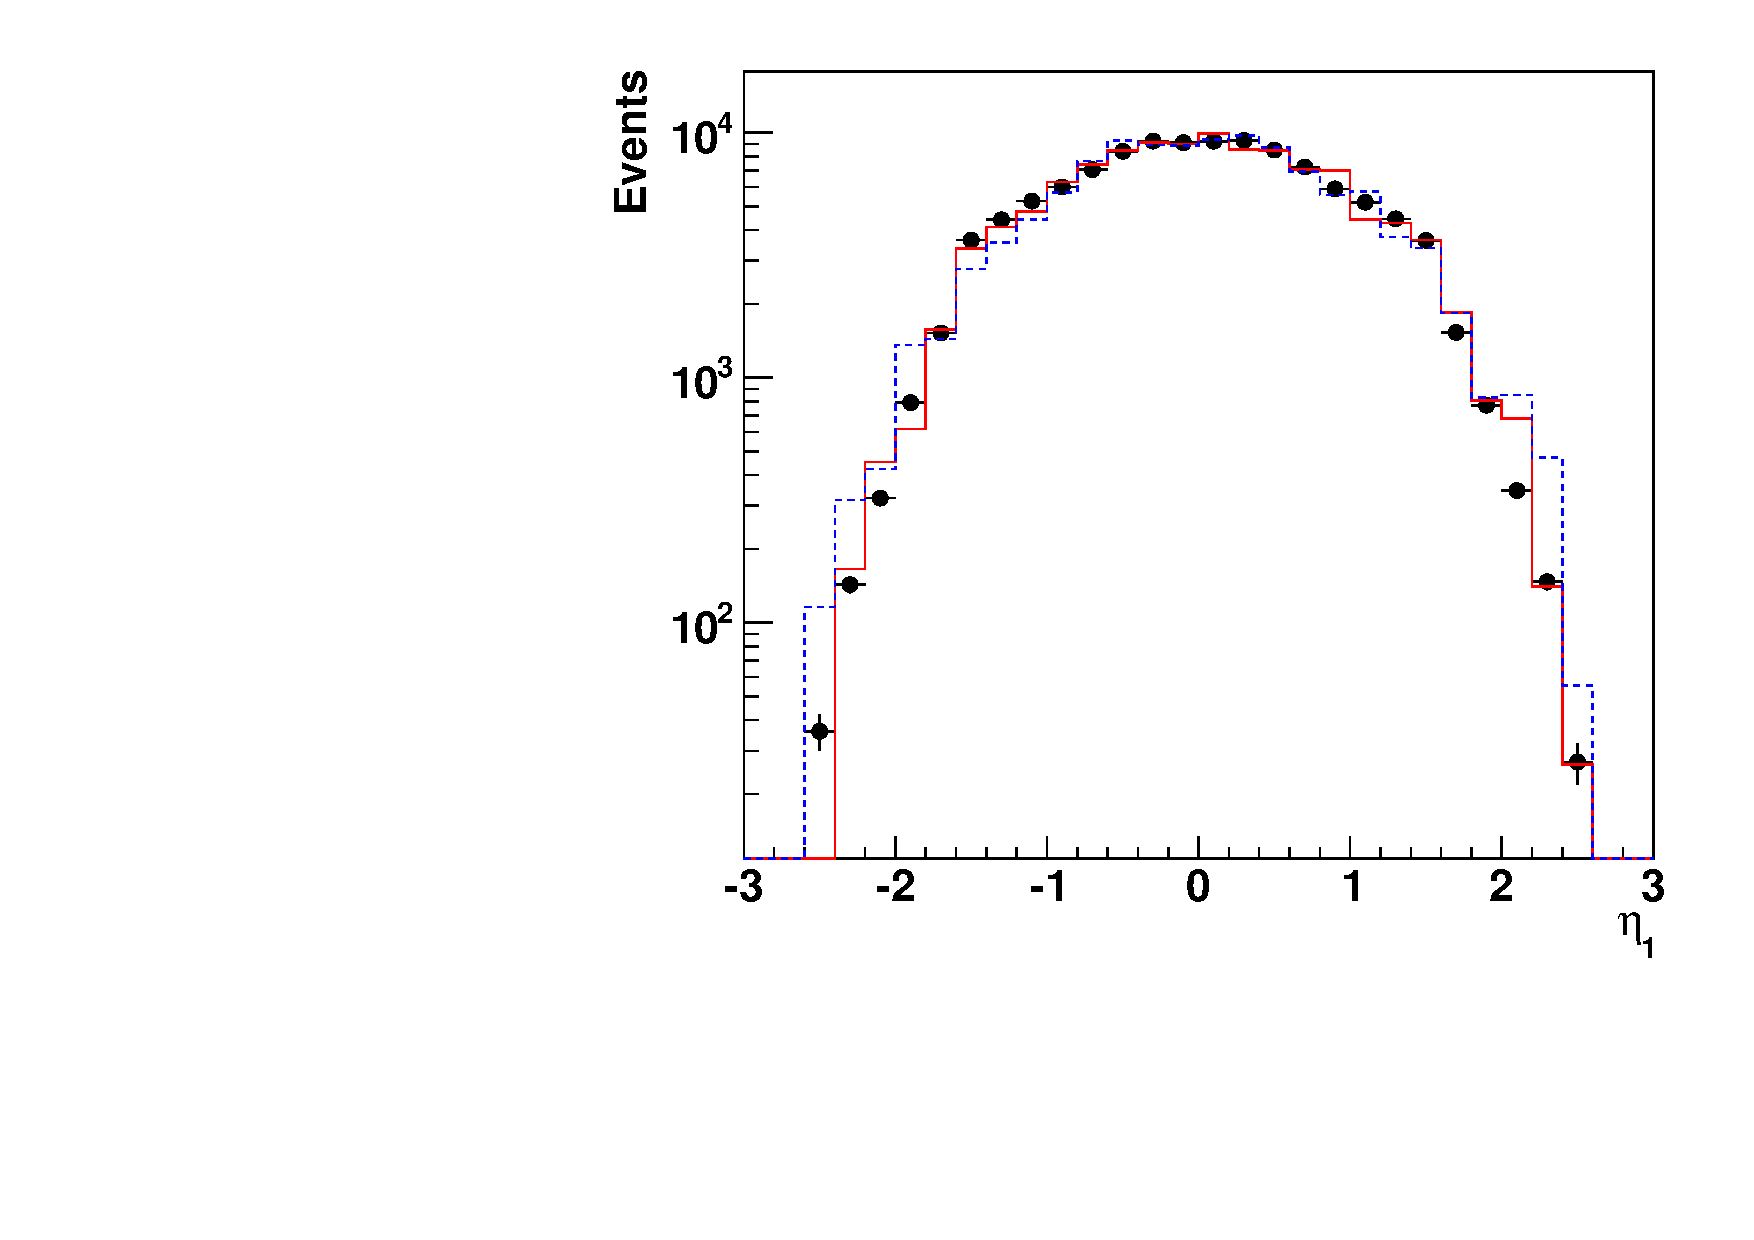
\includegraphics{EXO-12-024/figs/Data-MC-comparisons/Eta1-qVLowP.pdf}} &
     \resizebox{0.5\linewidth}{!}{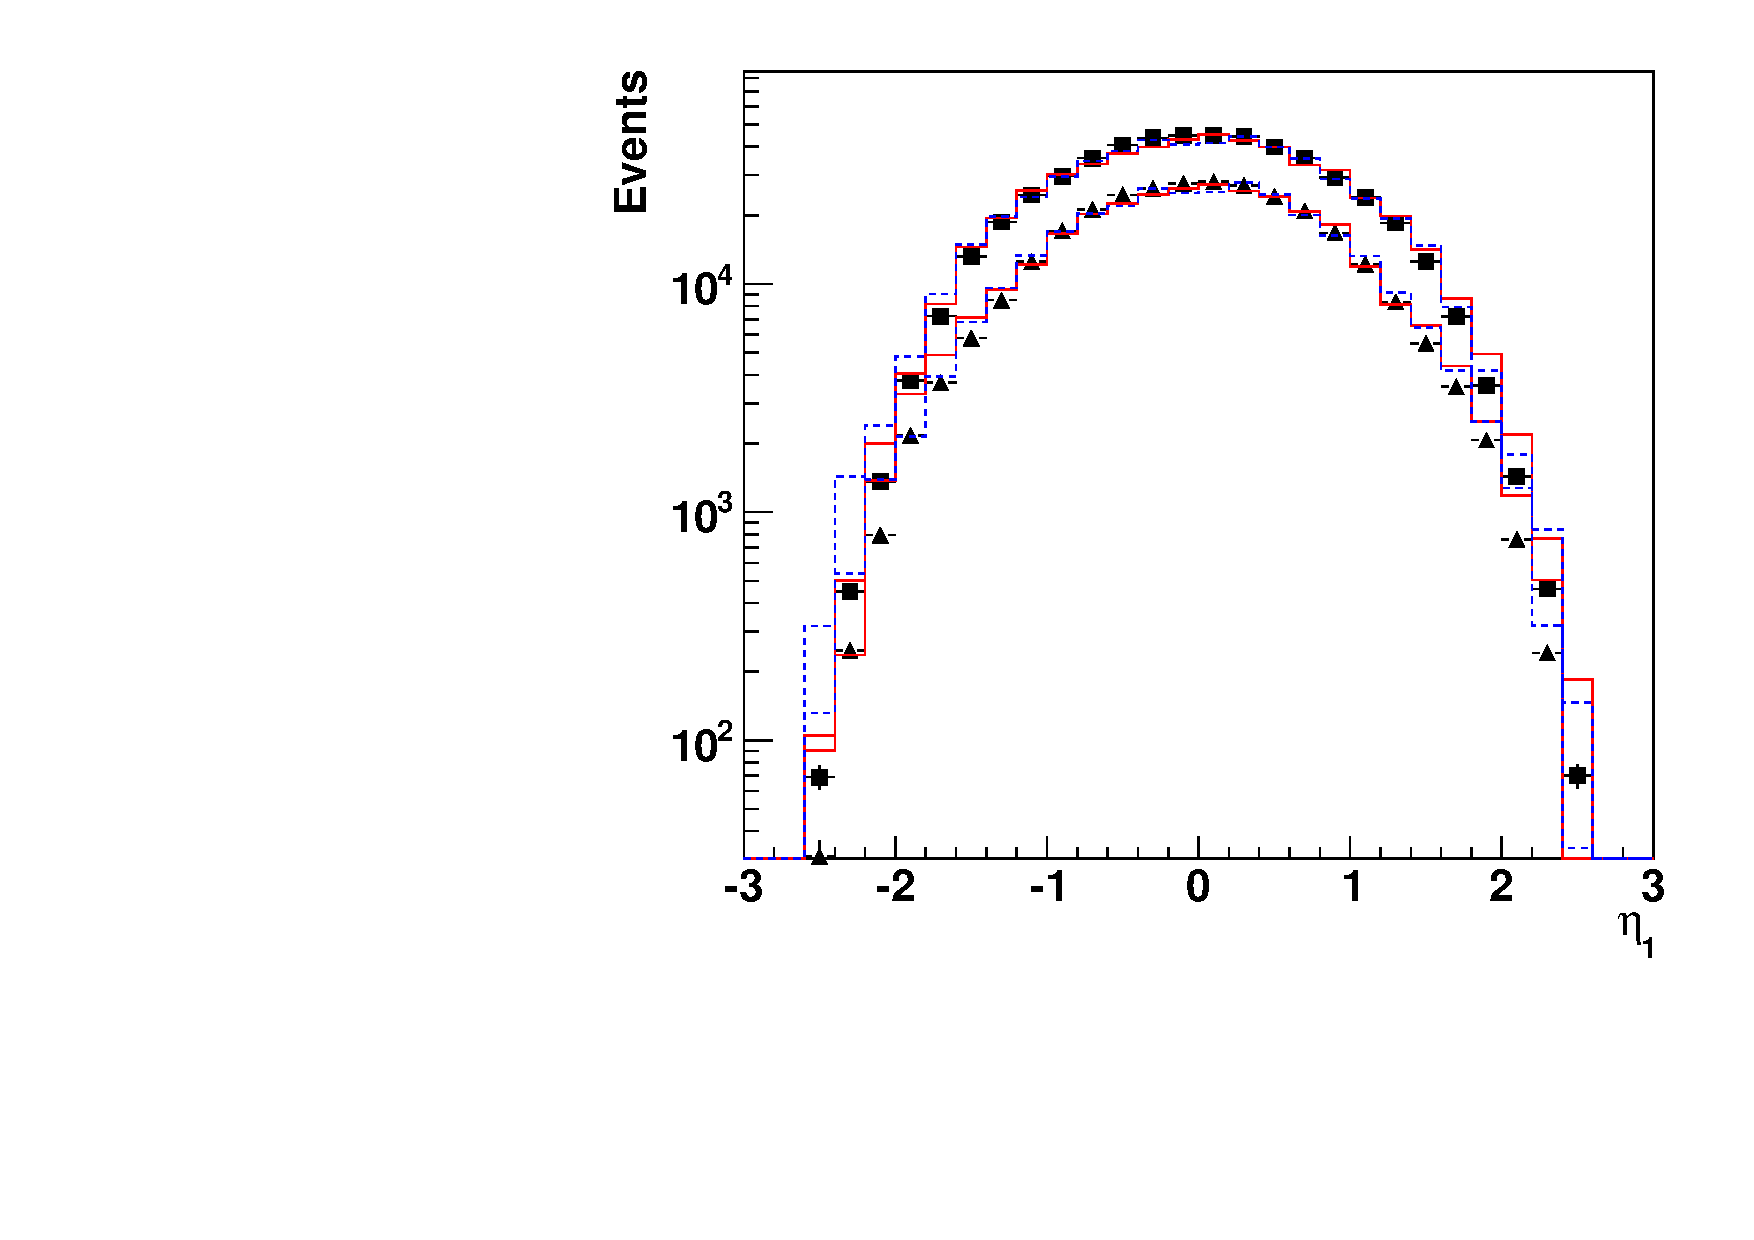
\includegraphics{EXO-12-024/figs/Data-MC-comparisons/Eta1-qVMiumHigh.pdf}} \\
\end{tabular}
  \caption[PT Single]{Comparisons between data and Monte Carlo
                    for $\eta$ of the second leading jet of low purity (left) and low-high purity (right) 1-tagged events.
	   The MC is normalized to the number of data events in each category. }
  \label{fig:Eta1Single}
\end{figure}

\begin{figure}[htb]
\centering
\begin{tabular}{cc}
     \resizebox{0.5\linewidth}{!}{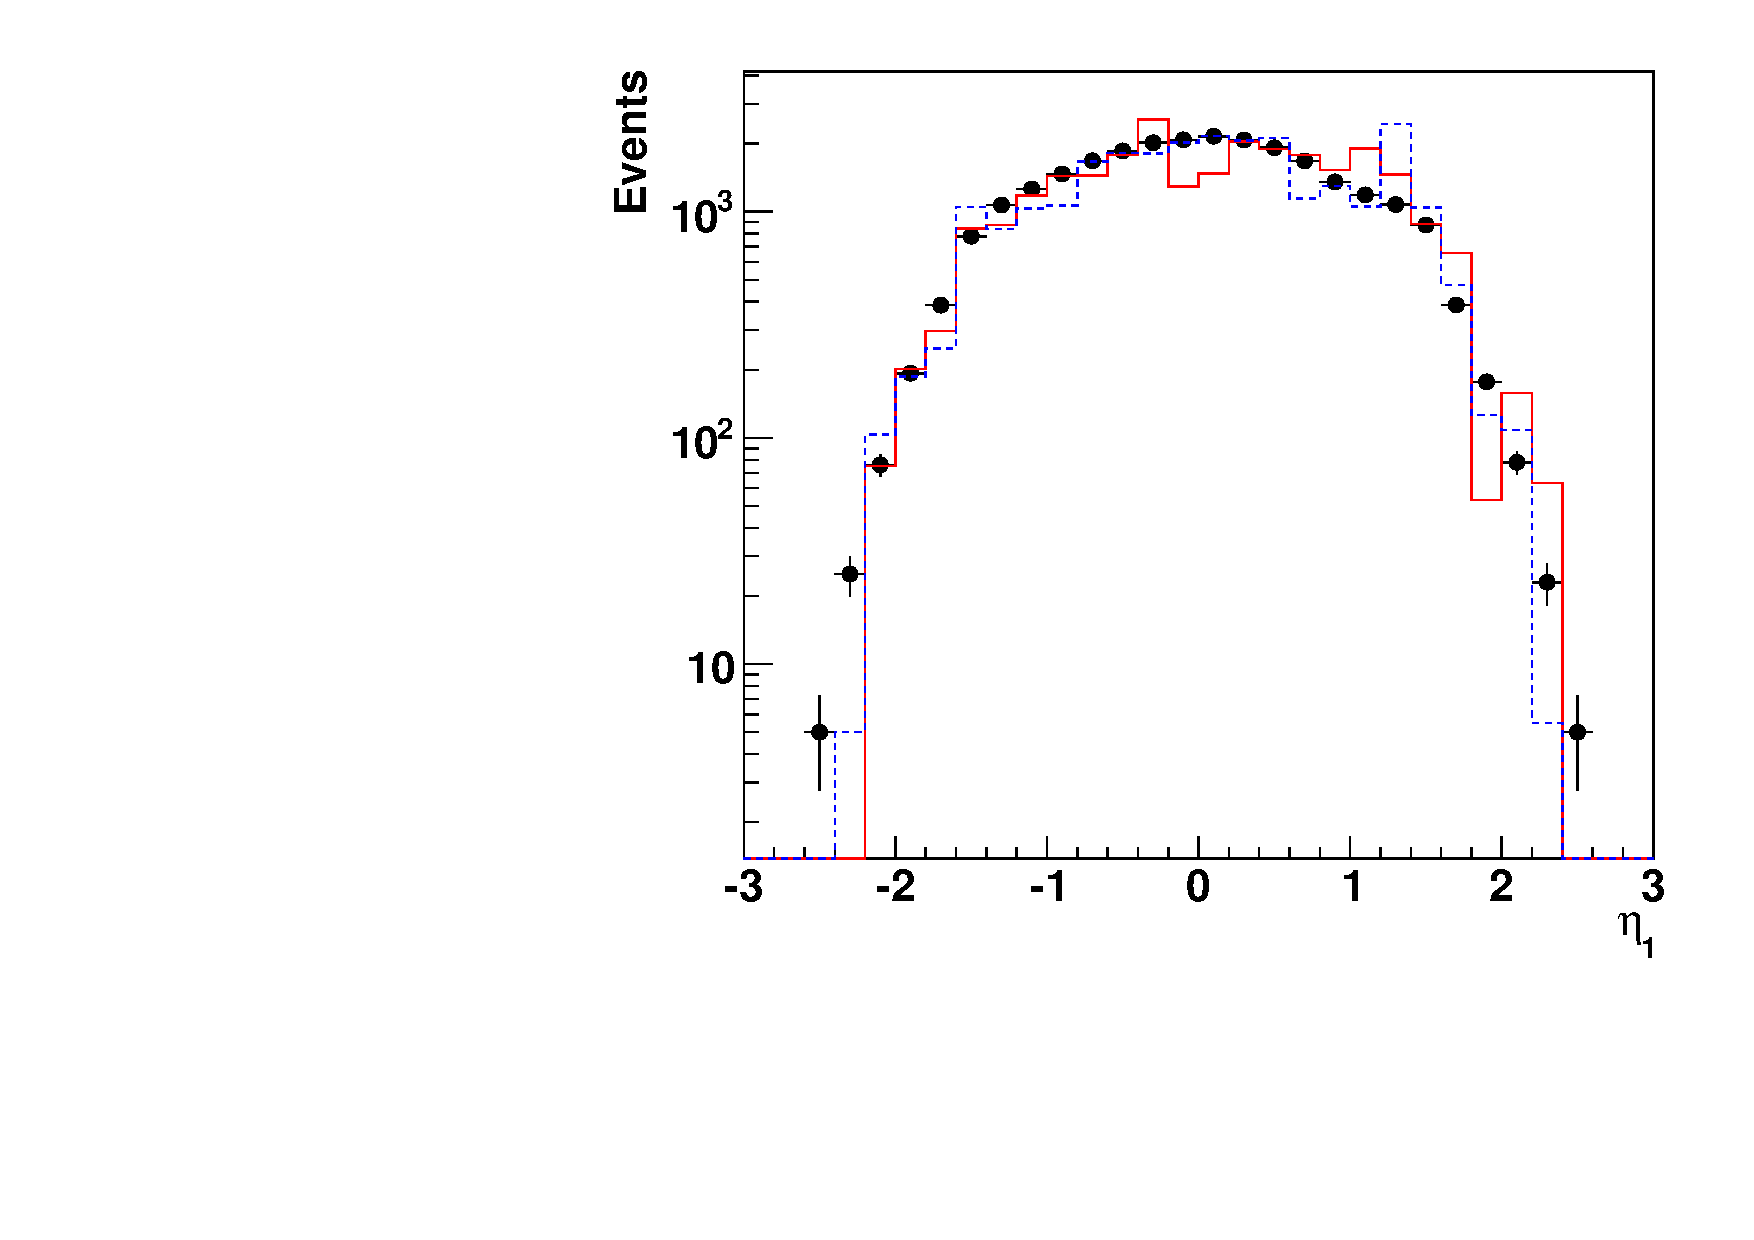
\includegraphics{EXO-12-024/figs/Data-MC-comparisons/Eta1-VVLowP.pdf}} &
     \resizebox{0.5\linewidth}{!}{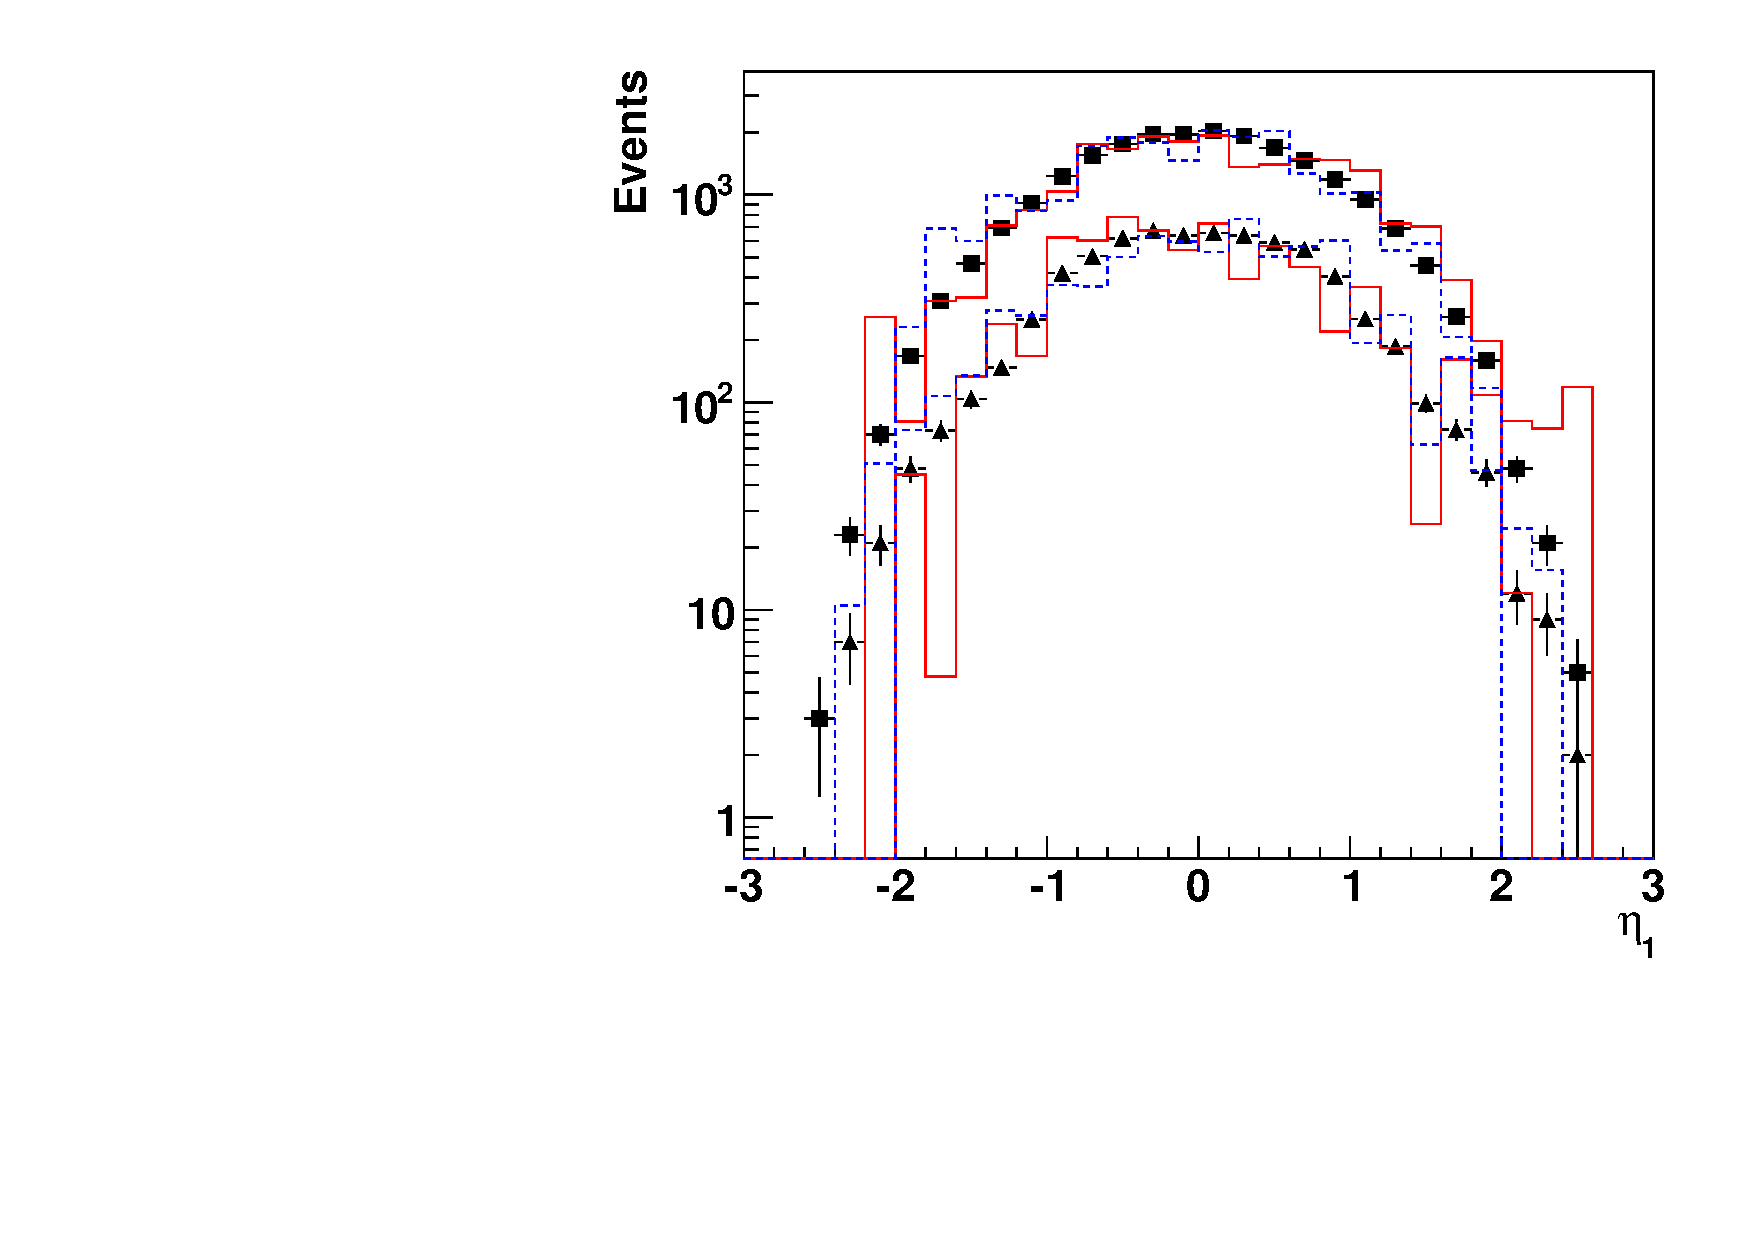
\includegraphics{EXO-12-024/figs/Data-MC-comparisons/Eta1-VVMiumHigh.pdf}} \\
\end{tabular}
  \caption[Delta Eta Double]{Comparisons between data and Monte Carlo
                     for $\eta$ of the second leading jet of low purity (left) and low-high purity (right) 2-tagged events. The MC is normalized to the number of data events in each category. }
  \label{fig:Eta1Double}
\end{figure}

%\newpage
%\begin{figure}[htb]
%\centering
%\begin{tabular}{cc}
%     \resizebox{0.5\linewidth}{!}{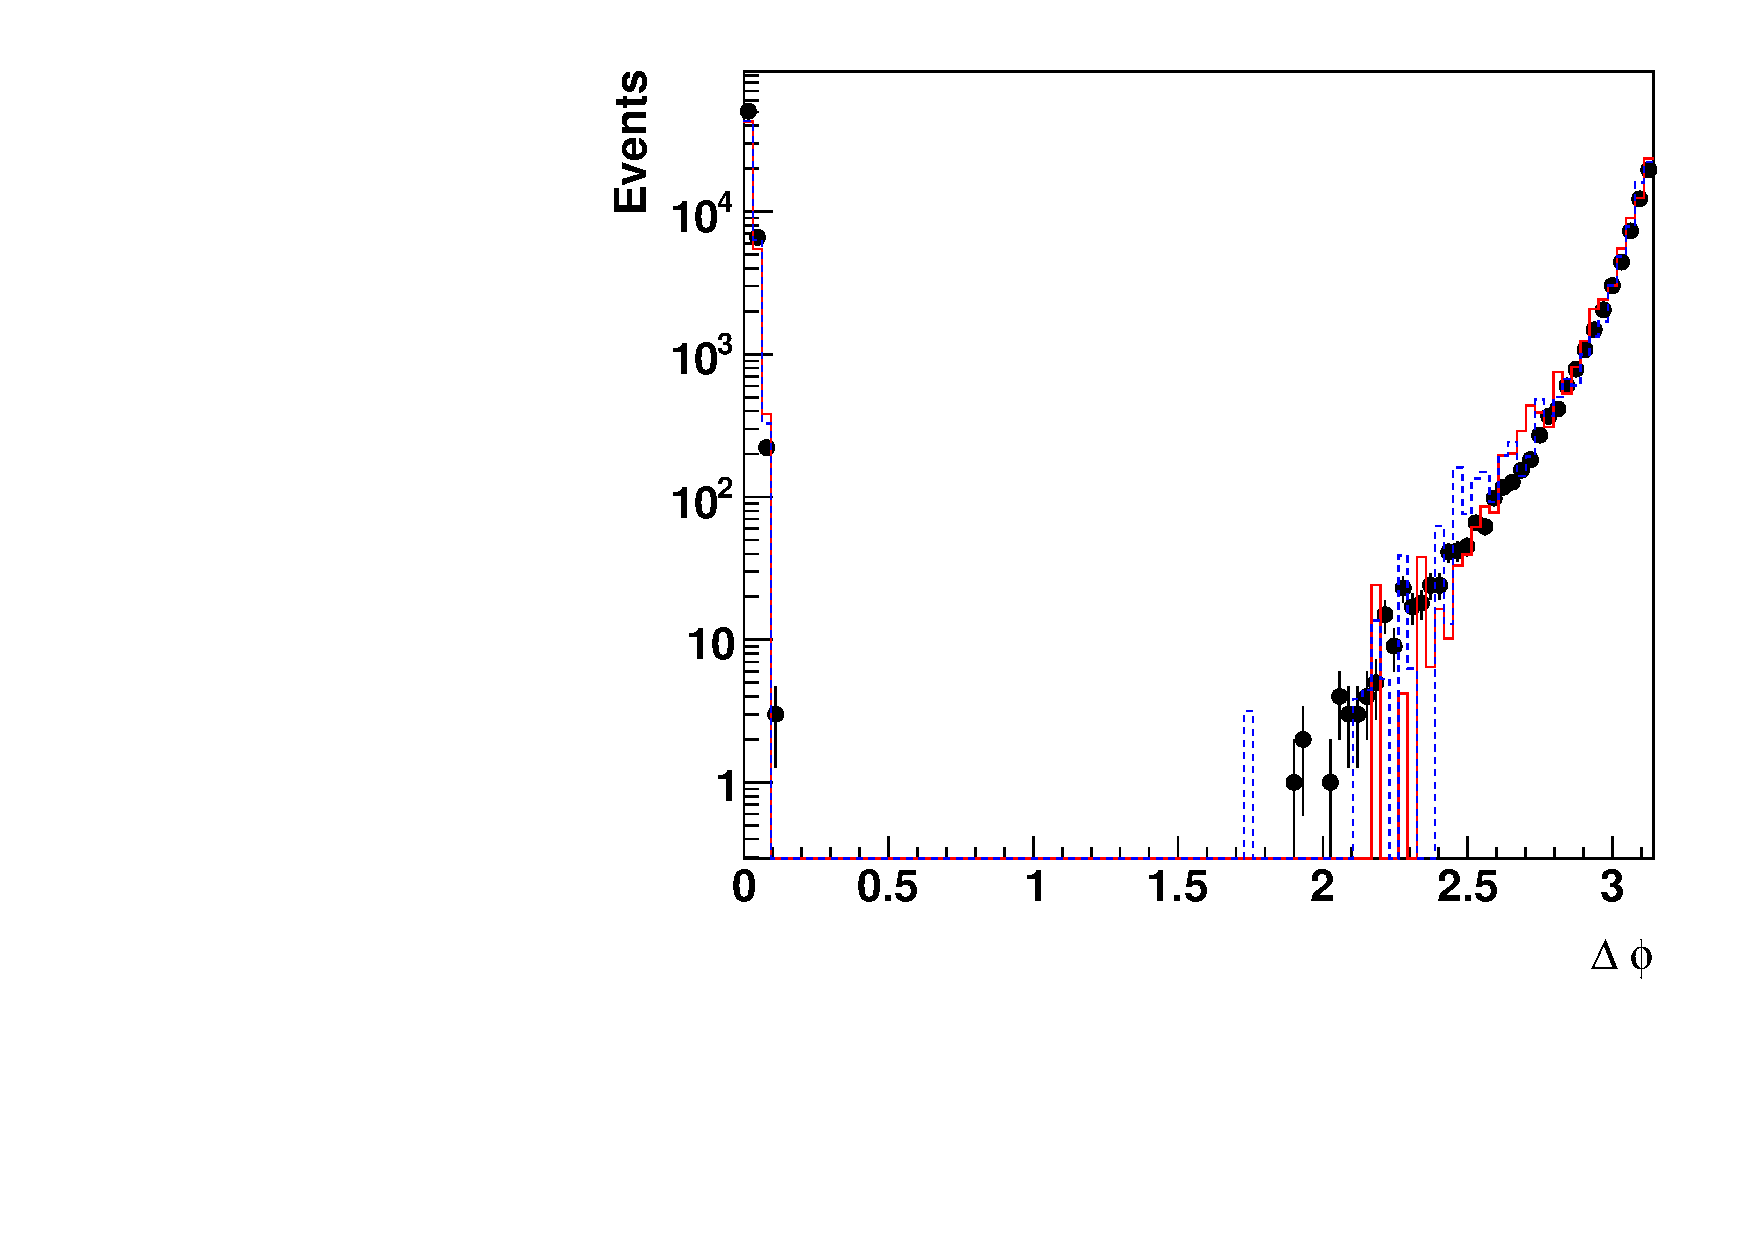
\includegraphics{EXO-12-024/figs/Data-MC-comparisons/CA8CA8-qVLowP.pdf}} &
%     \resizebox{0.5\linewidth}{!}{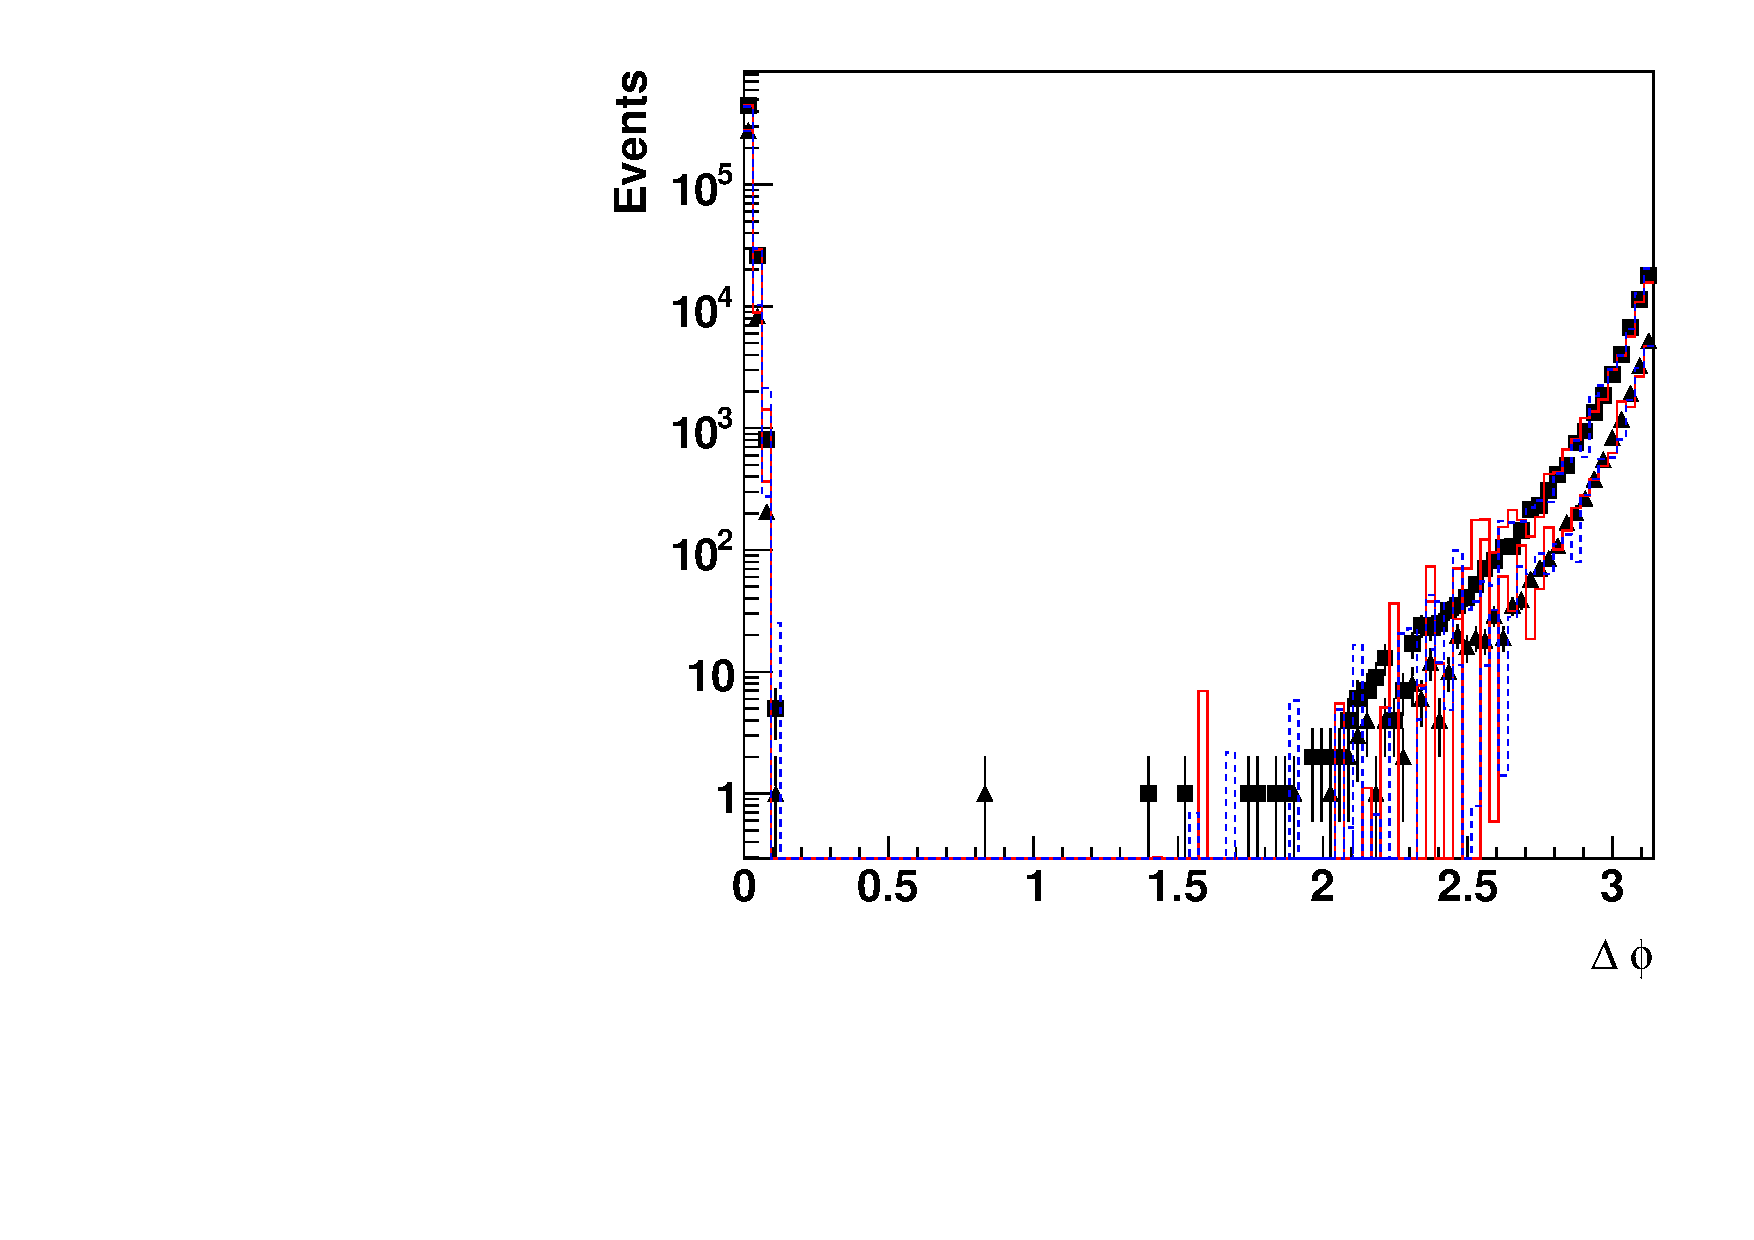
\includegraphics{EXO-12-024/figs/Data-MC-comparisons/CA8CA8-qVMiumHigh.pdf}} \\
%\end{tabular}
%  \caption[PT Single]{Comparisons between data and Monte Carlo
%                    for $\Delta \phi$ of the leading ungroomed CA8 jet and leading pruned CA8 jet of low purity (left) and low-high purity (right) 1-tagged events.
%	   The MC is normalized to the number of data events in each category. }
%  \label{fig:CA8Single}
%\end{figure}

%\begin{figure}[htb]
%\centering
%\begin{tabular}{cc}
%     \resizebox{0.5\linewidth}{!}{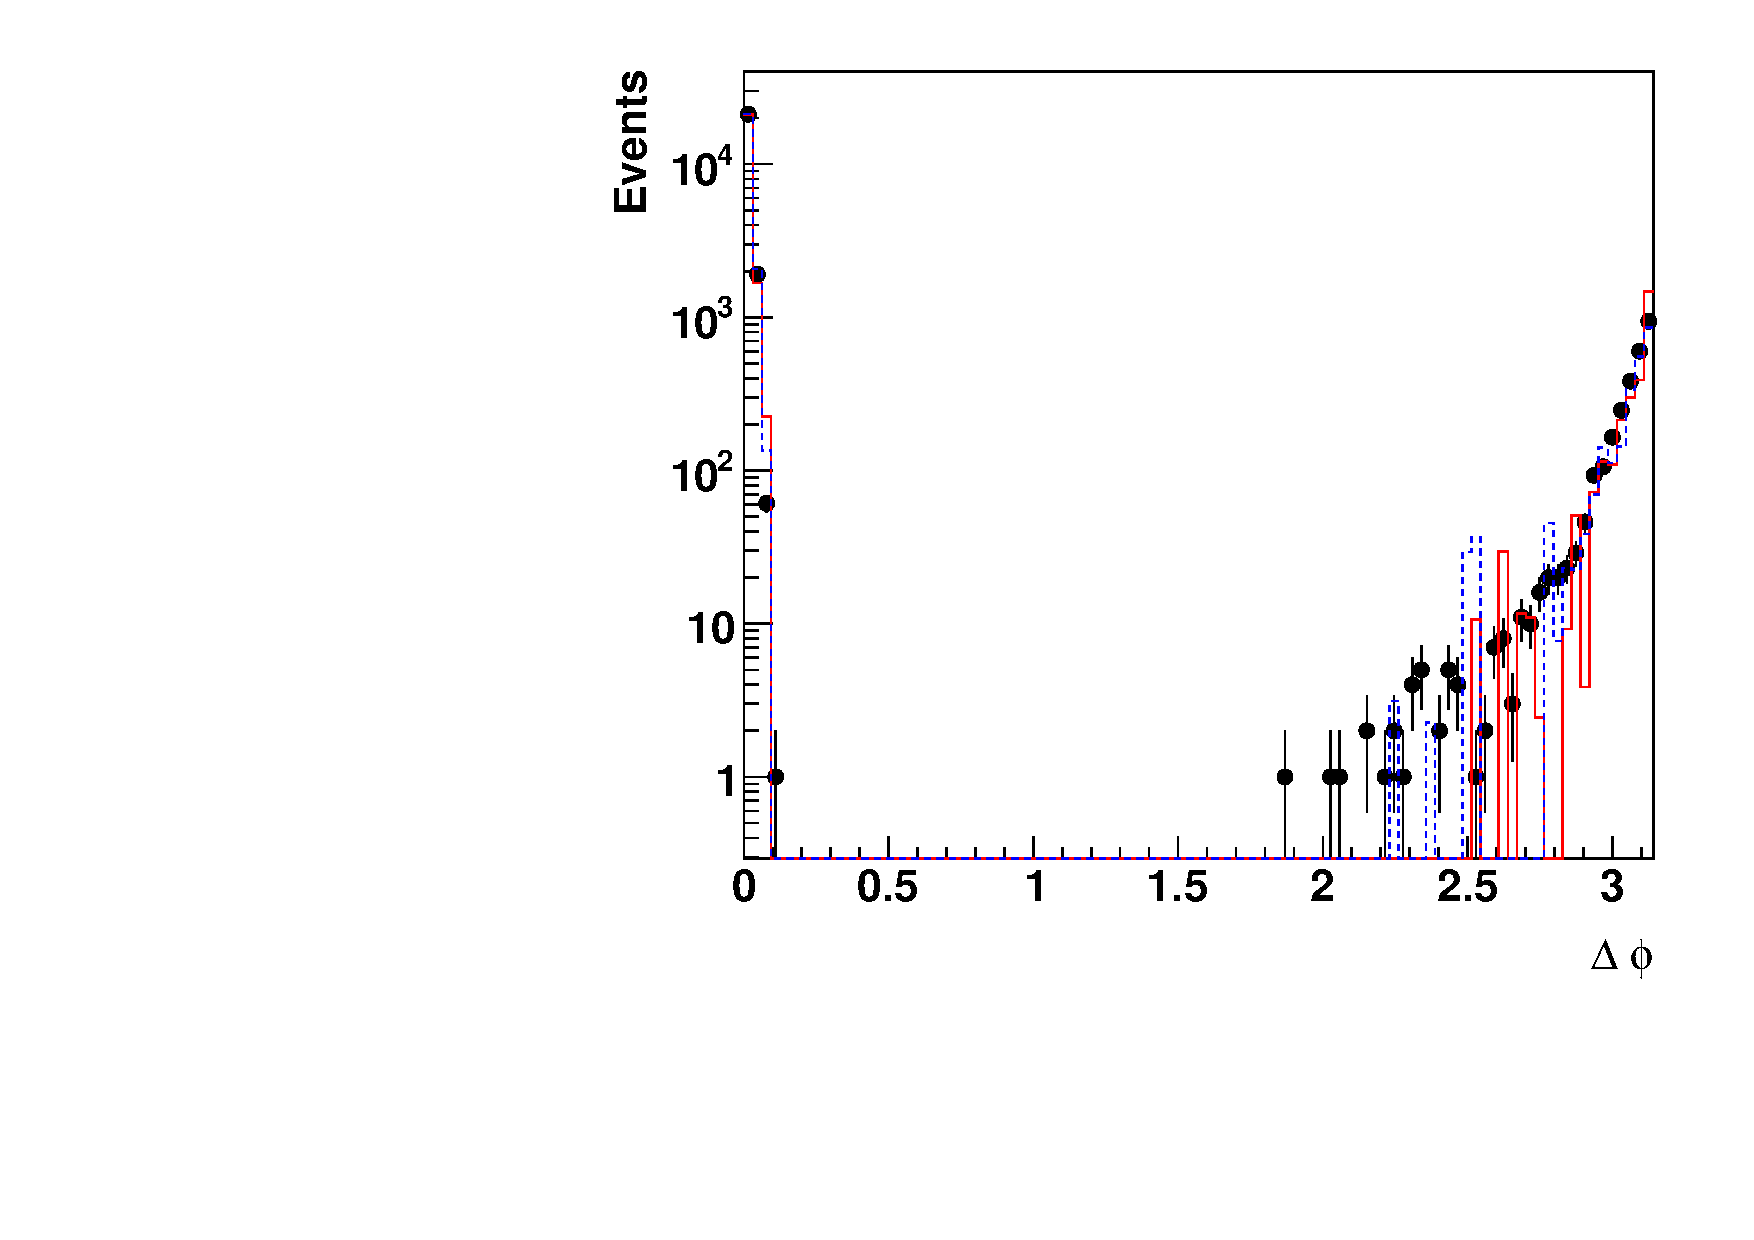
\includegraphics{EXO-12-024/figs/Data-MC-comparisons/CA8CA8-VVLowP.pdf}} &
%     \resizebox{0.5\linewidth}{!}{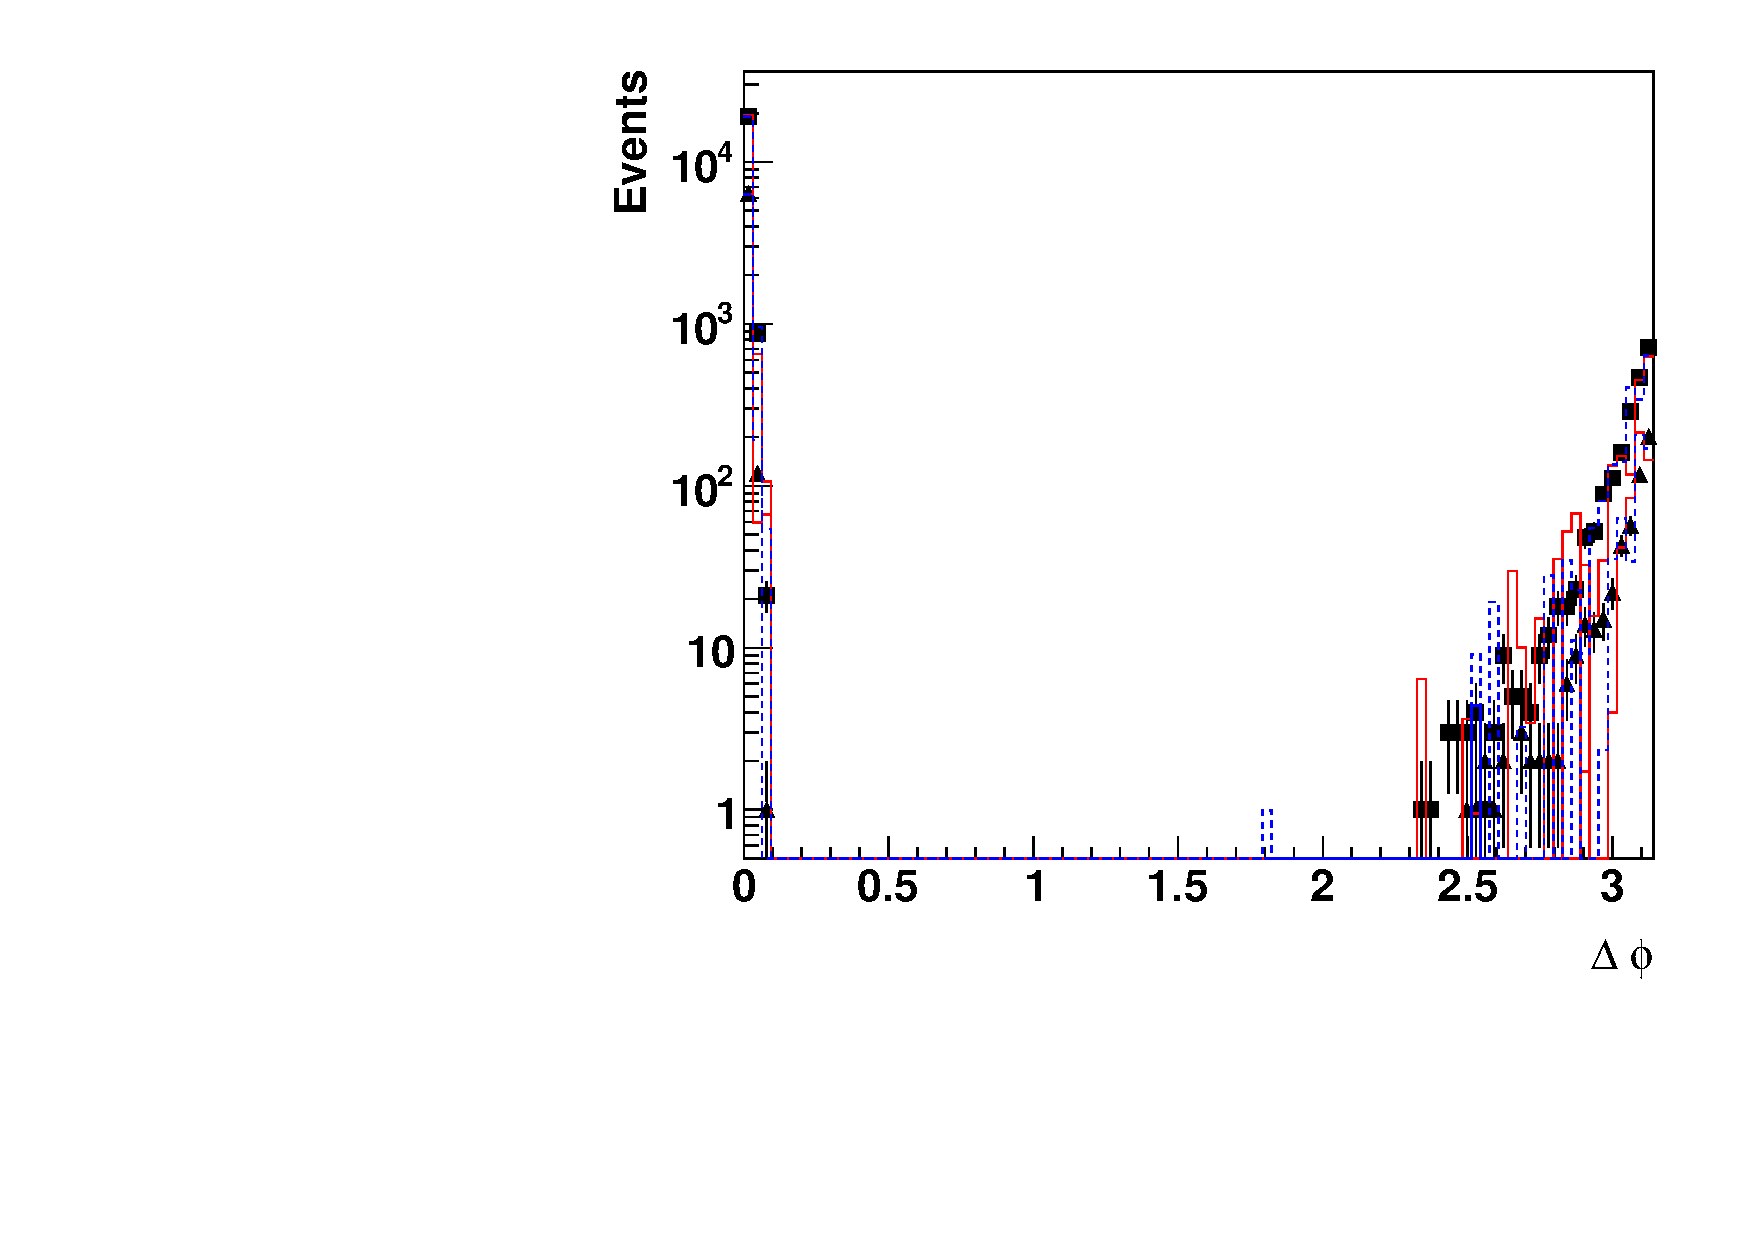
\includegraphics{EXO-12-024/figs/Data-MC-comparisons/CA8CA8-VVMiumHigh.pdf}} \\
%\end{tabular}
%  \caption[PT Single]{Comparisons between data and Monte Carlo
%                    for $\Delta \phi$ of the leading ungroomed CA8 jet and leading pruned CA8 jet of low purity (left) and low-high purity (right) 2-tagged events.
%           The MC is normalized to the number of data events in each category. }
%  \label{fig:CA8Double}
%\end{figure}


\newpage
\begin{figure}[htb]
\centering
\begin{tabular}{cc}
     \resizebox{0.5\linewidth}{!}{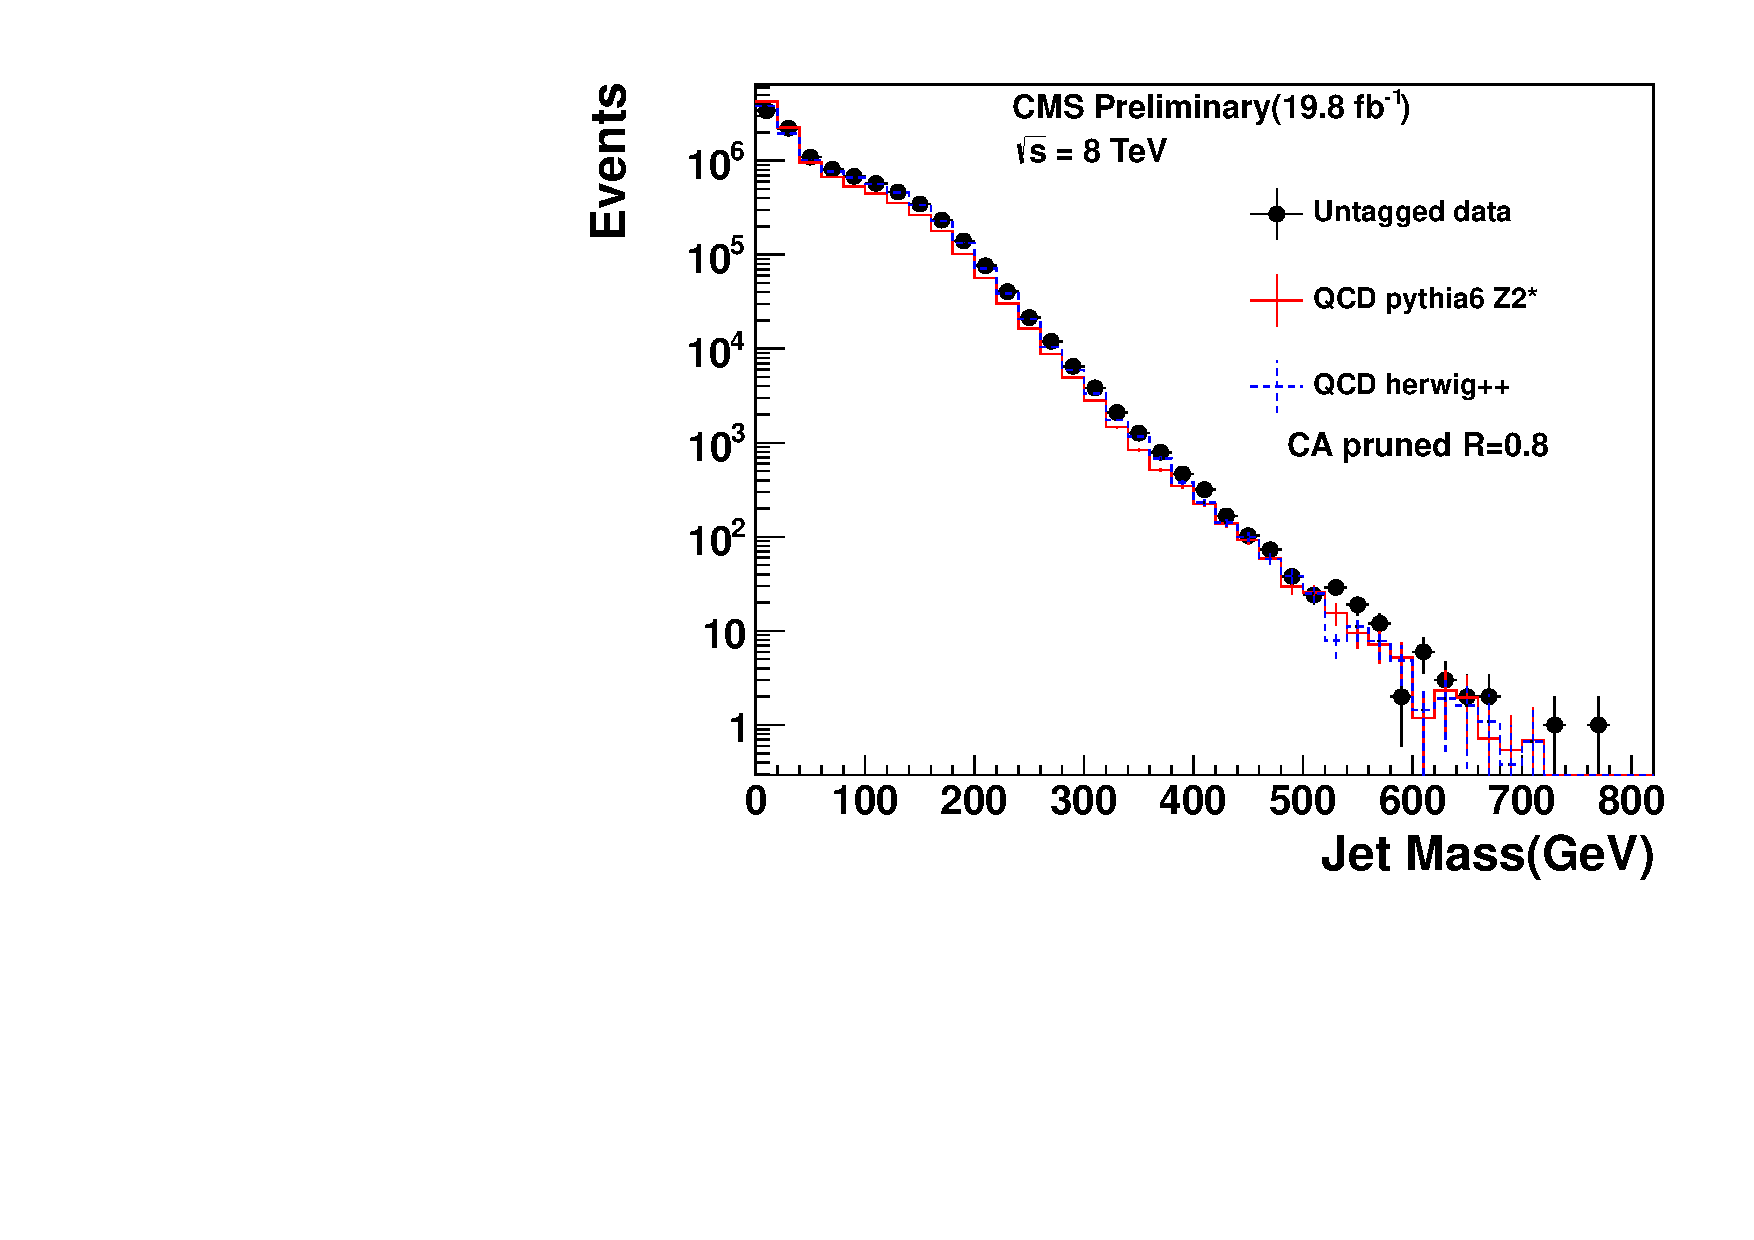
\includegraphics{EXO-12-024/figs/Data-MC-comparisons/lumi19fb_dataMC_ca8jet_norm_mlog.pdf}} &
     \resizebox{0.5\linewidth}{!}{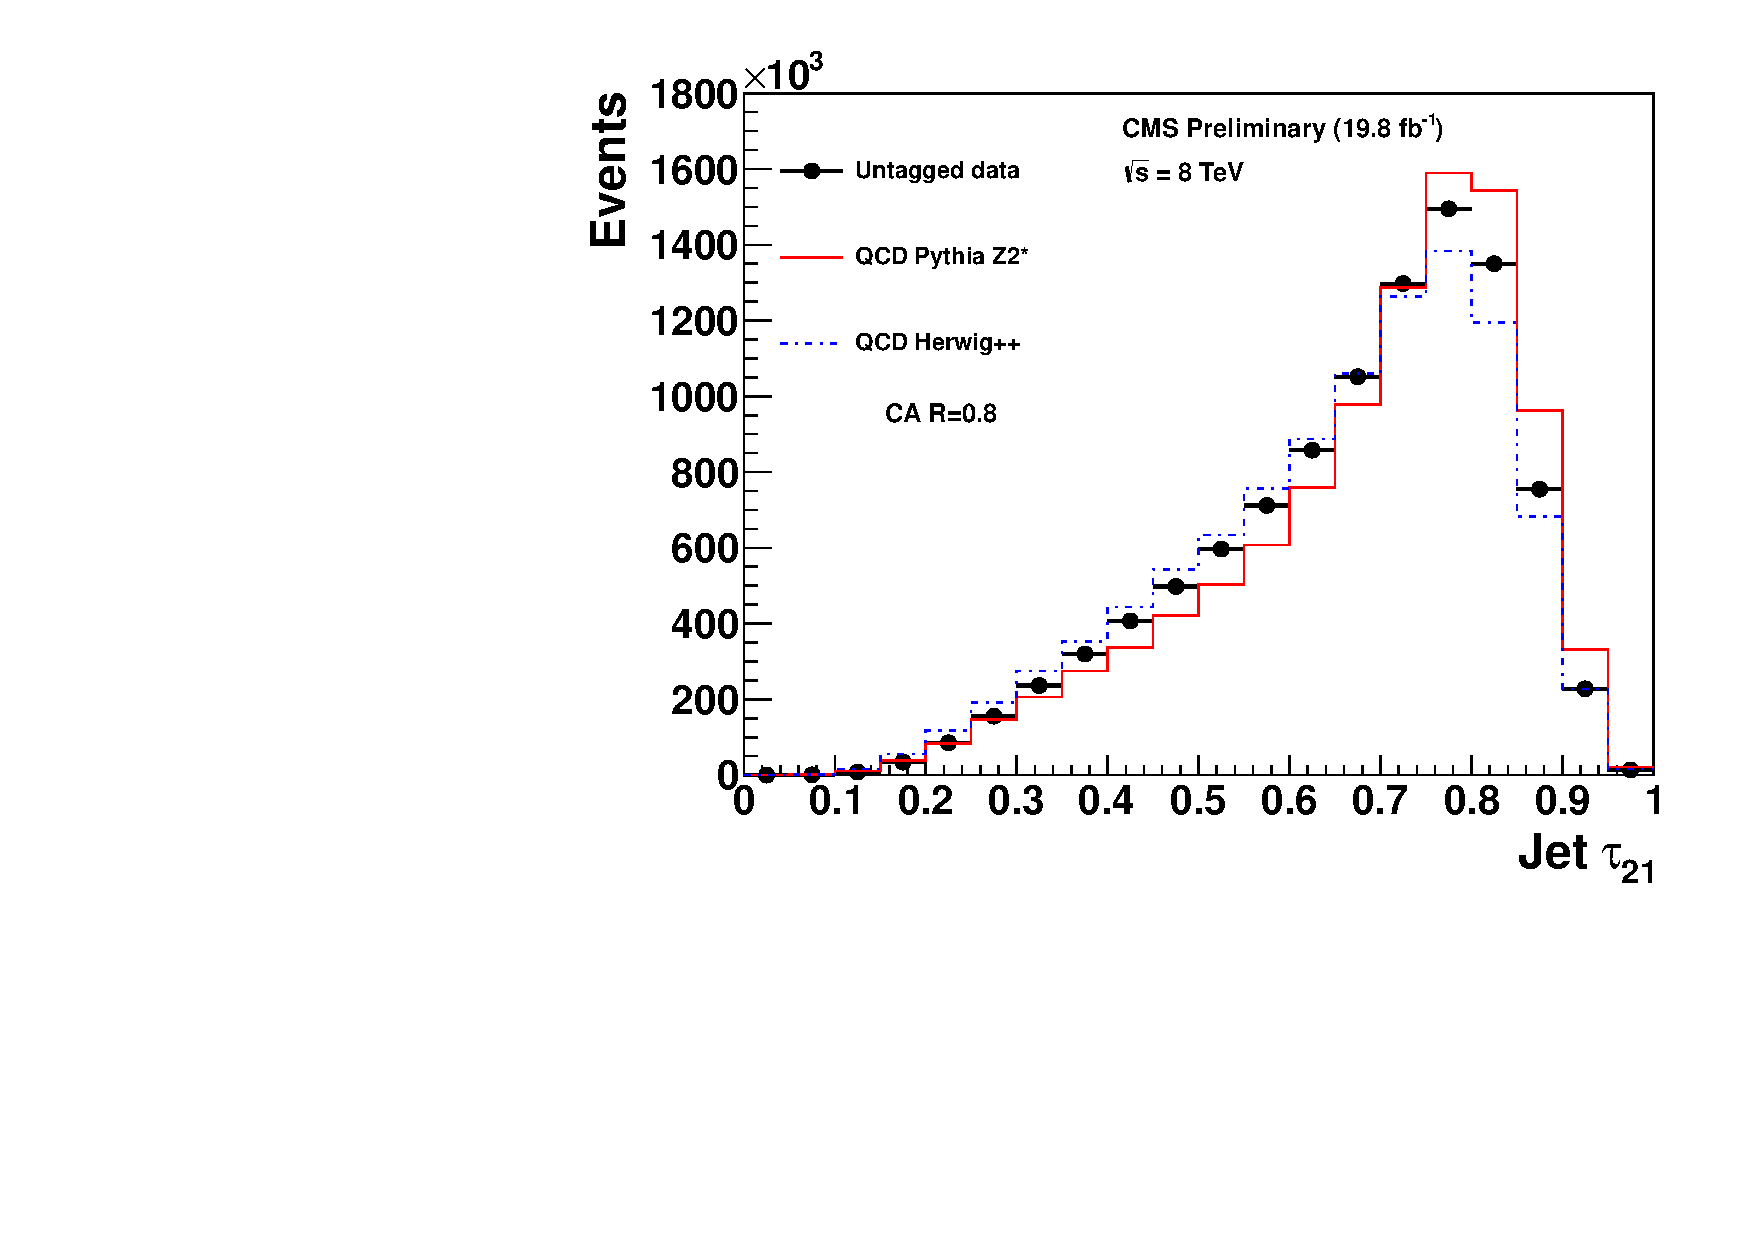
\includegraphics{EXO-12-024/figs/Data-MC-comparisons/data-qcd-Jet-Tau21.pdf}}\\
\end{tabular}
  \caption[Leading two jets mass]{Comparisons between data and Monte Carlo for
                    mass(left) and $\tau_{21}$(right) of the leading two jets.
	   The MC is normalized to the number of data events in each category.}
  \label{fig:massNsub}
\end{figure}



















\newpage

\begin{figure}[htb]
\centering
\begin{tabular}{cc}
     \resizebox{0.5\linewidth}{!}{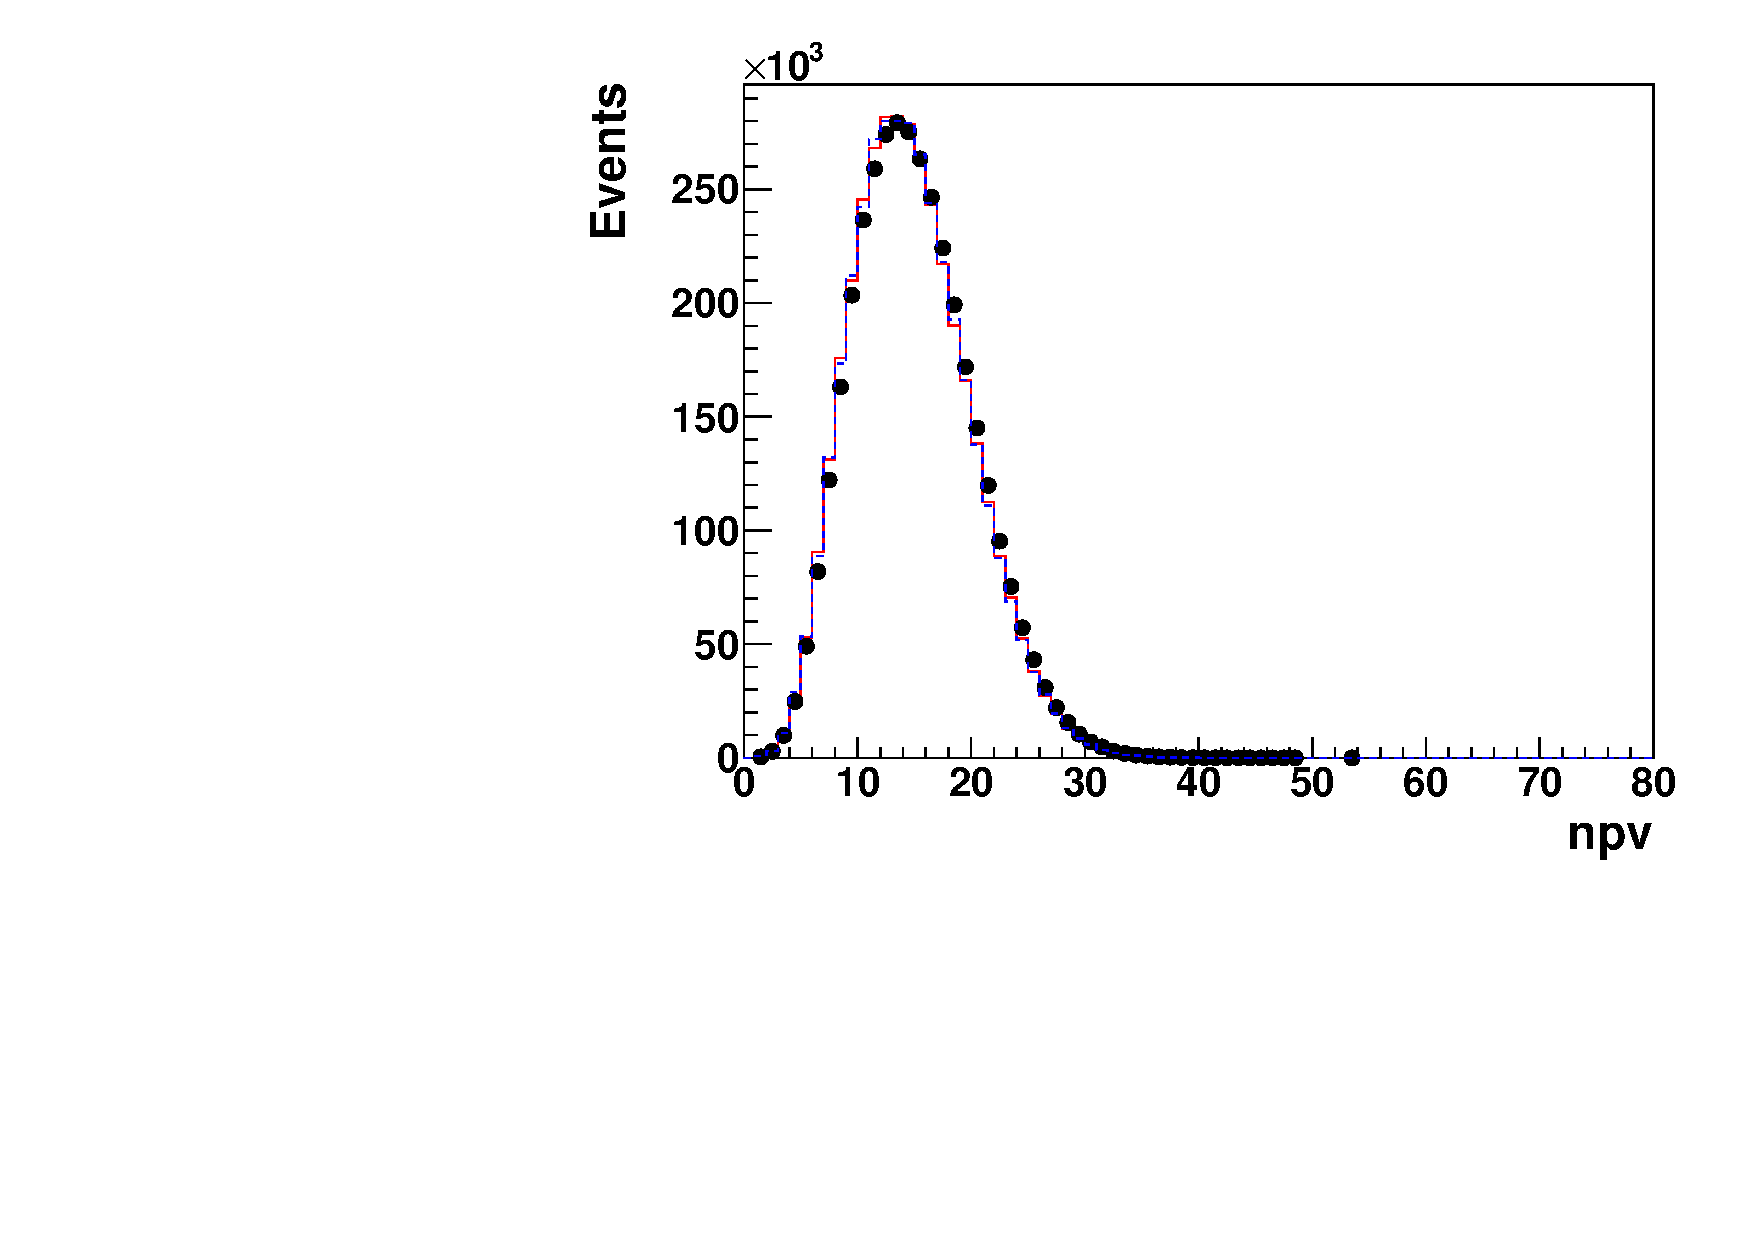
\includegraphics{EXO-12-024/figs/Data-MC-comparisons/npv.pdf}} &
     \resizebox{0.5\linewidth}{!}{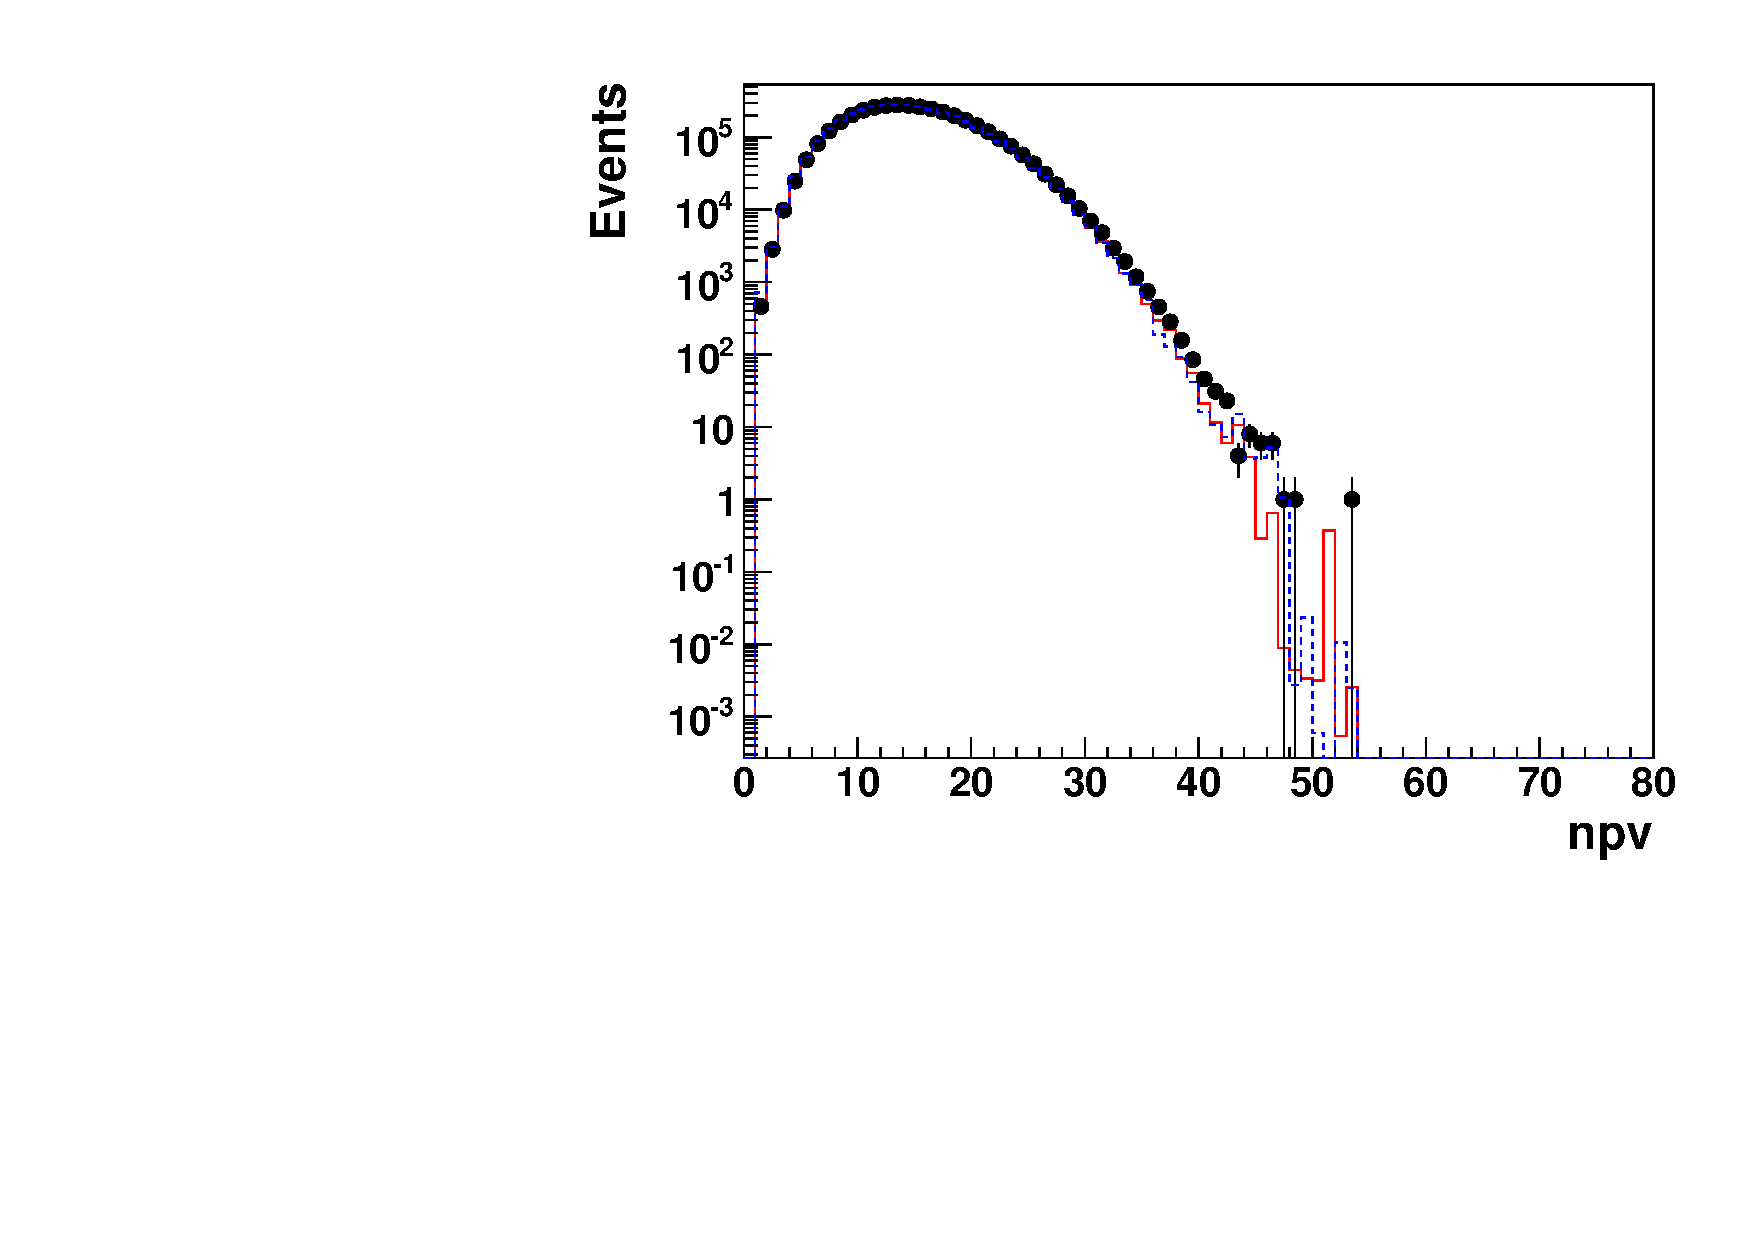
\includegraphics{EXO-12-024/figs/Data-MC-comparisons/npvlog.pdf}} \\
\end{tabular}
  \caption[Leading two jets mass drop]{Comparisons between data and Monte Carlo for
                   number of primary vertice to show the effect on Monte Carlo after pile up reweighting. 
	   The MC is normalized to the number of data events. Plot on the right is the log scale plot. (The plot includes only a subset of the full data sample.)}
  \label{fig:npv}
\end{figure}

\begin{figure}[htb]
\centering
\begin{tabular}{cc}
     \resizebox{0.5\linewidth}{!}{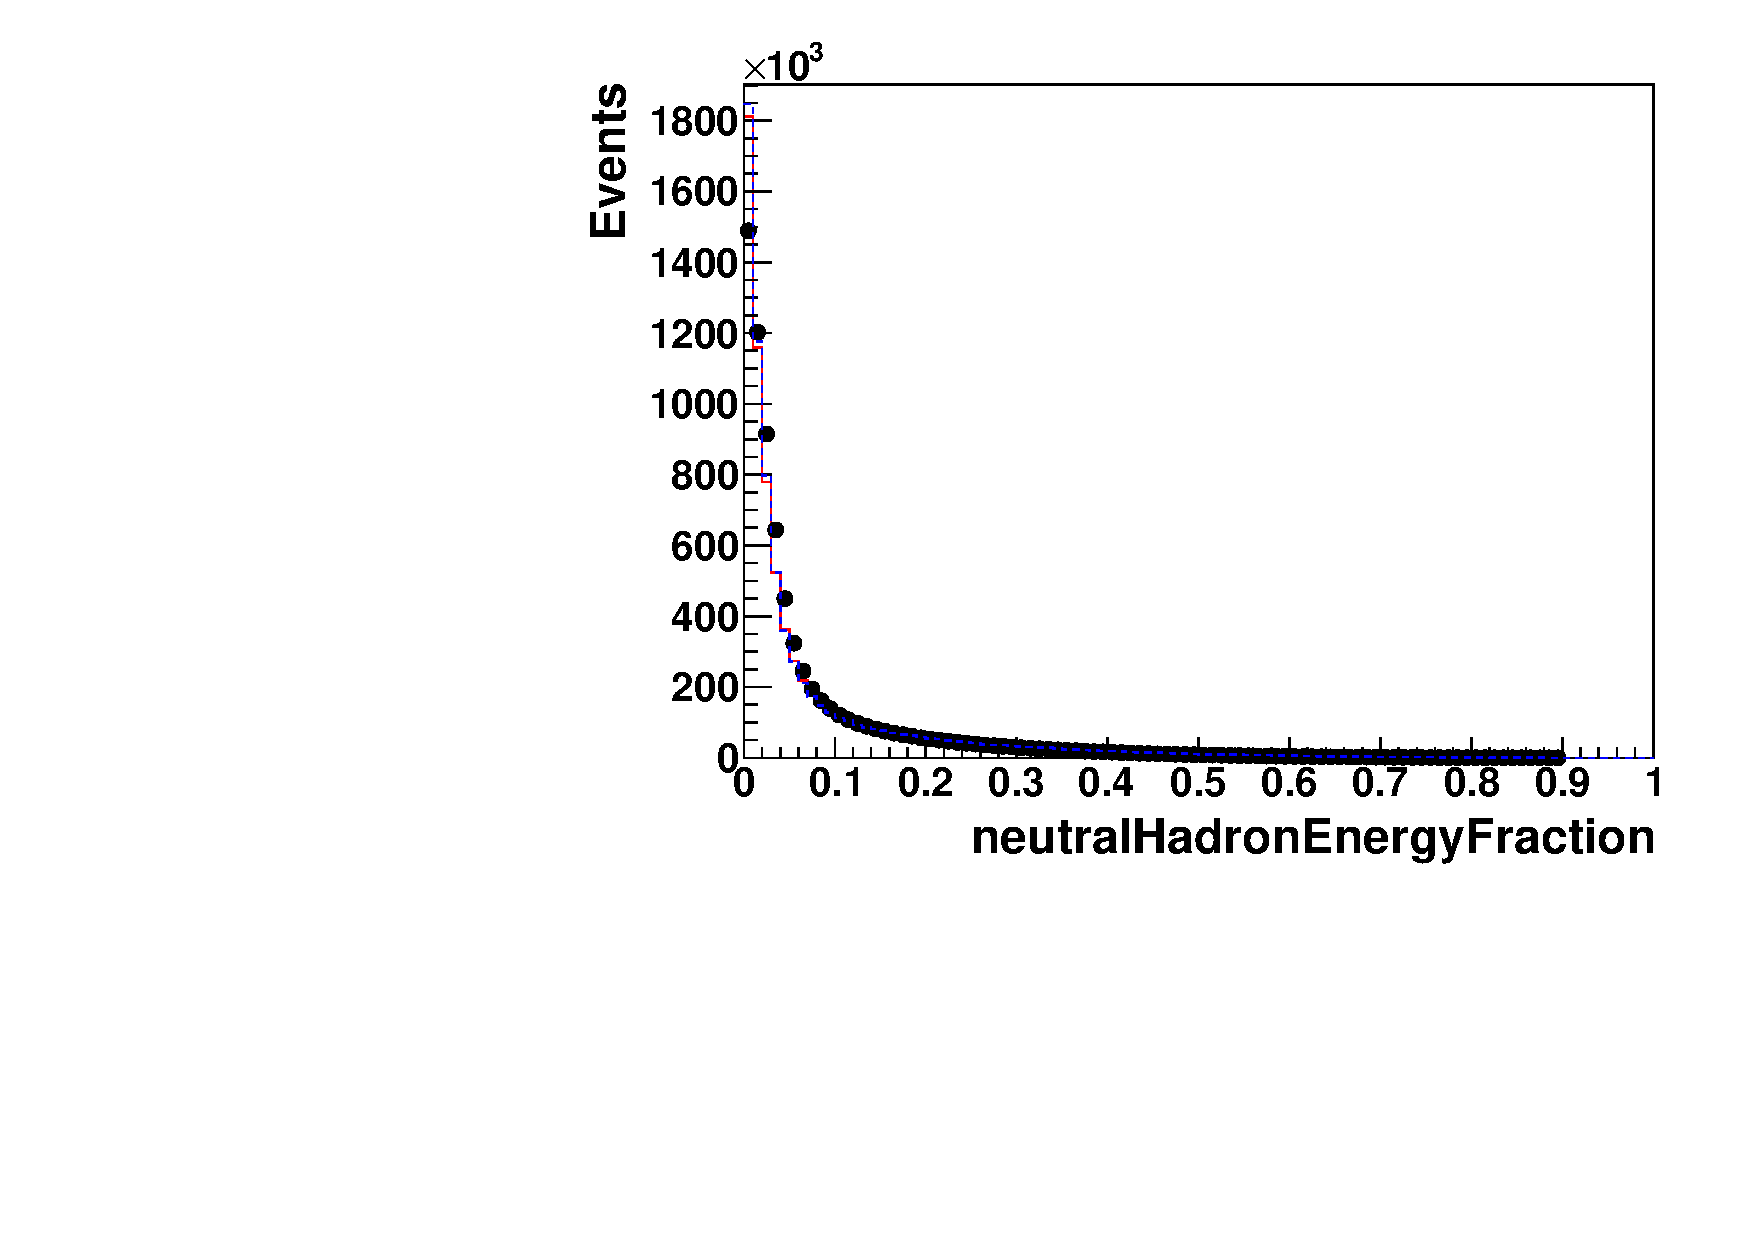
\includegraphics{EXO-12-024/figs/Data-MC-comparisons/neutralHadronEnergyFraction.pdf}} &
     \resizebox{0.5\linewidth}{!}{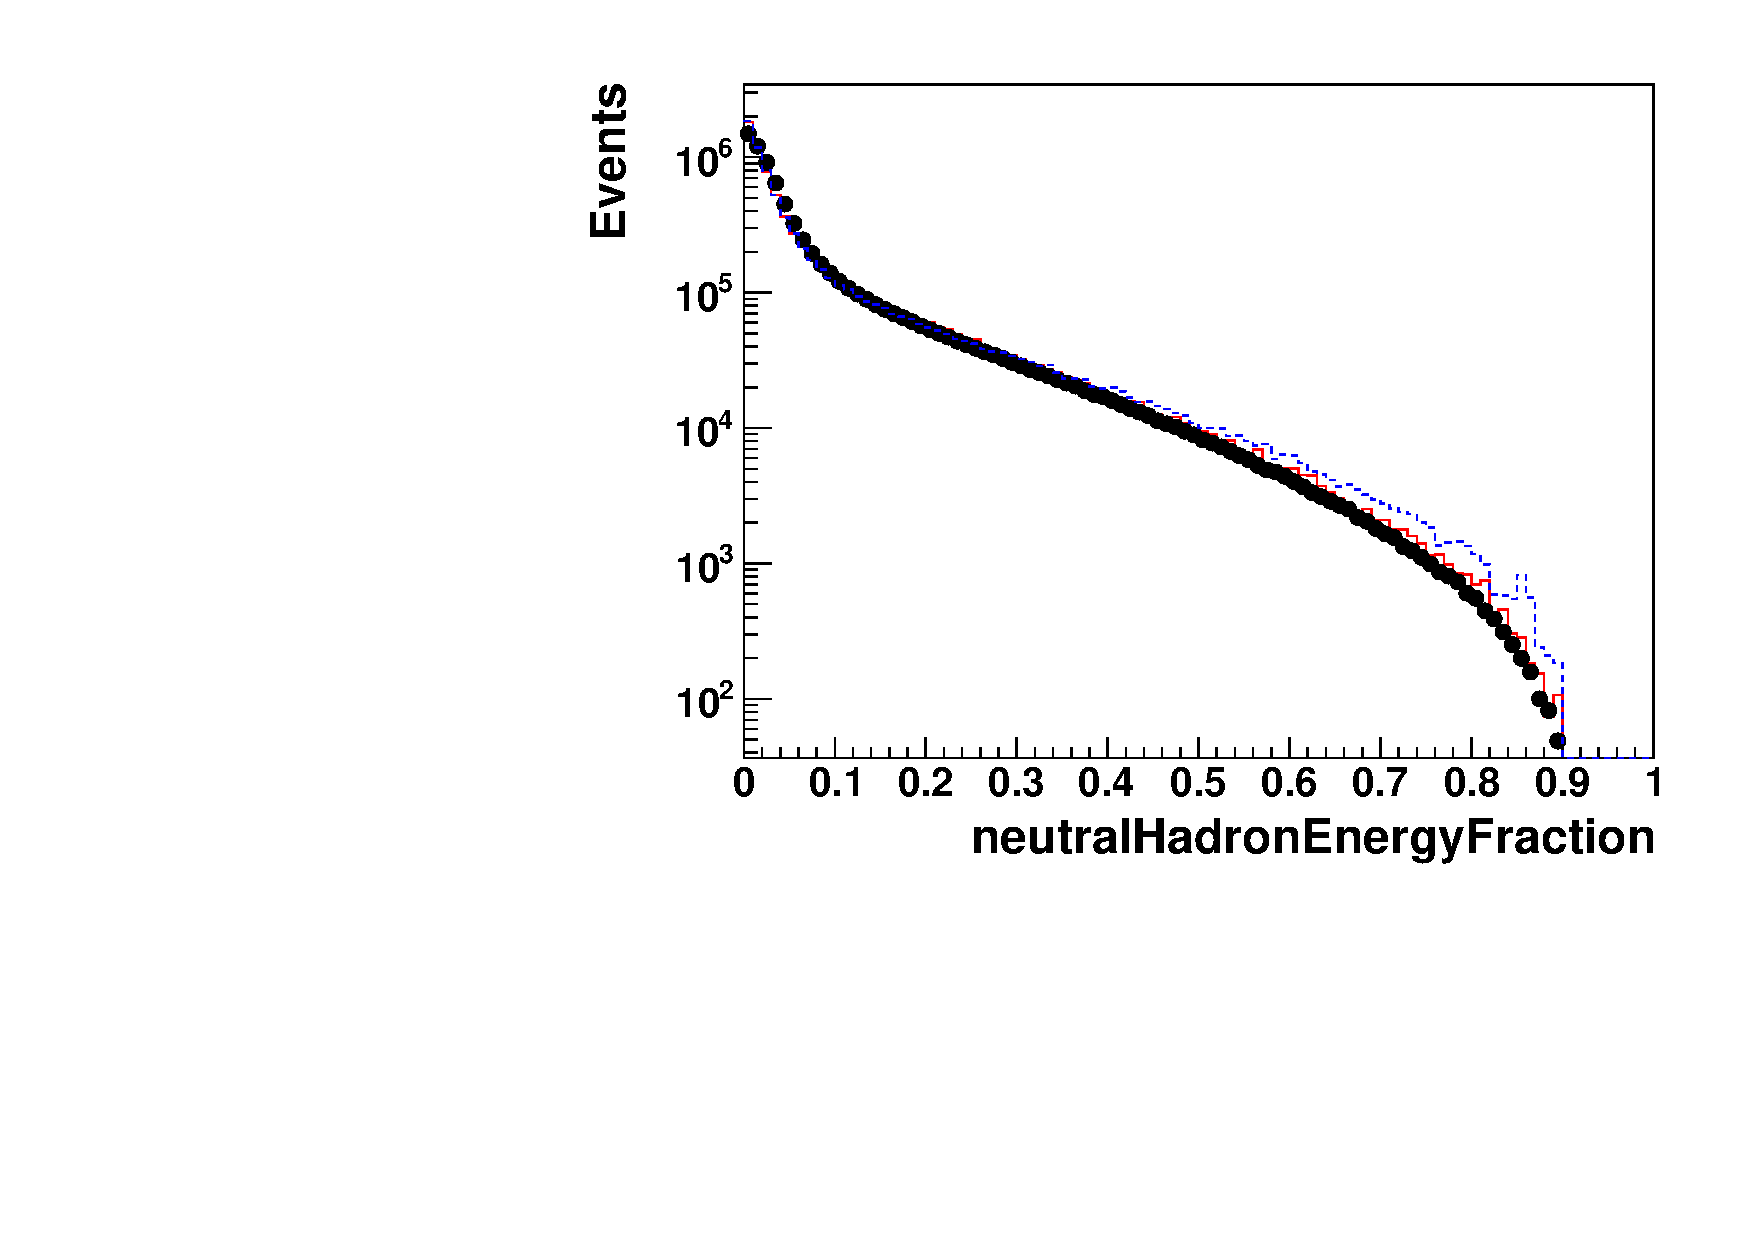
\includegraphics{EXO-12-024/figs/Data-MC-comparisons/neutralHadronEnergyFractionlog.pdf}} \\
\end{tabular}
  \caption[Leading two jets mass drop]{Comparisons between data and Monte Carlo for neutral hadron energy fraction.  
	   The MC is normalized to the number of data events. Plot on the right is the log scale plot. (The plot includes only a subset of the full data sample.)}
  \label{fig:neutralHadronEnergyFraction}
\end{figure}

\clearpage
\newpage

\begin{figure}[htb]
\centering
\begin{tabular}{cc}
     \resizebox{0.5\linewidth}{!}{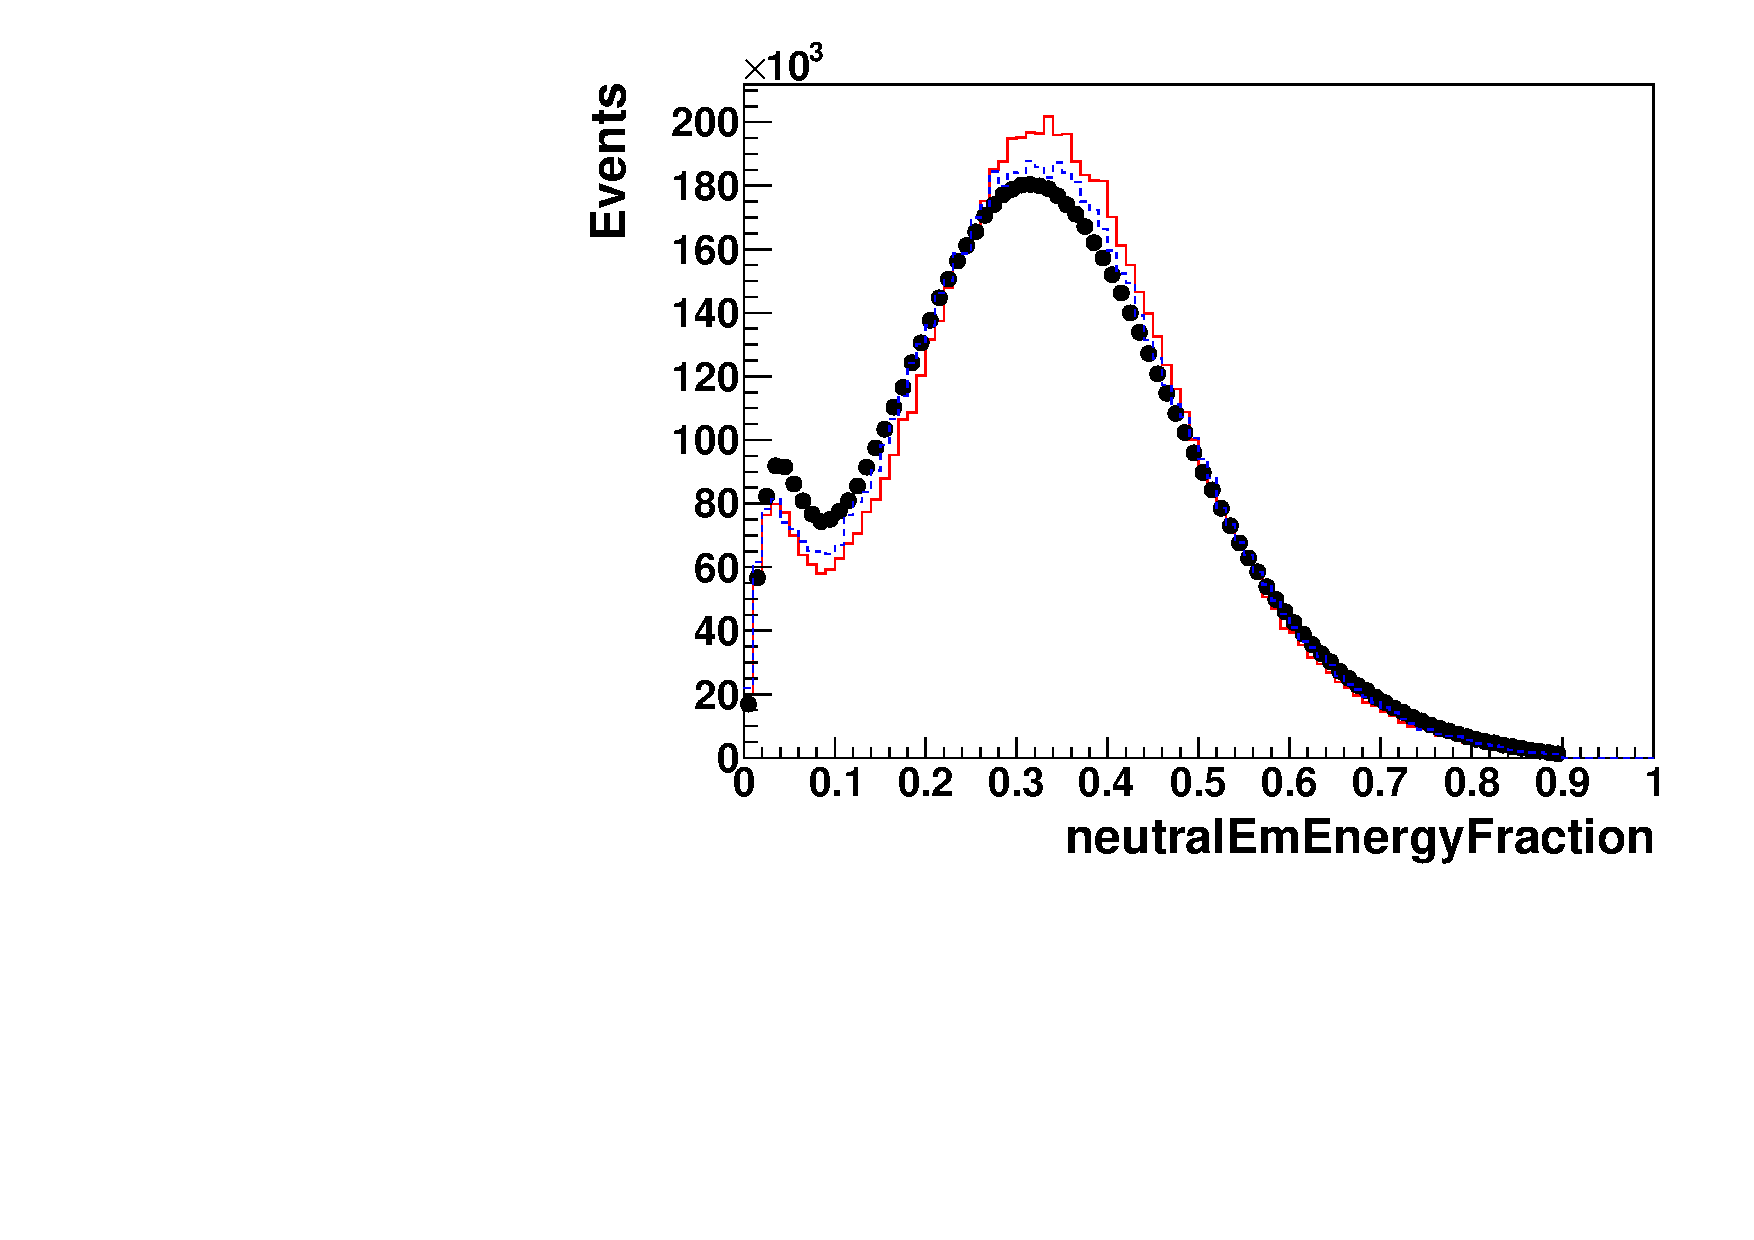
\includegraphics{EXO-12-024/figs/Data-MC-comparisons/neutralEmEnergyFraction.pdf}} &
     \resizebox{0.5\linewidth}{!}{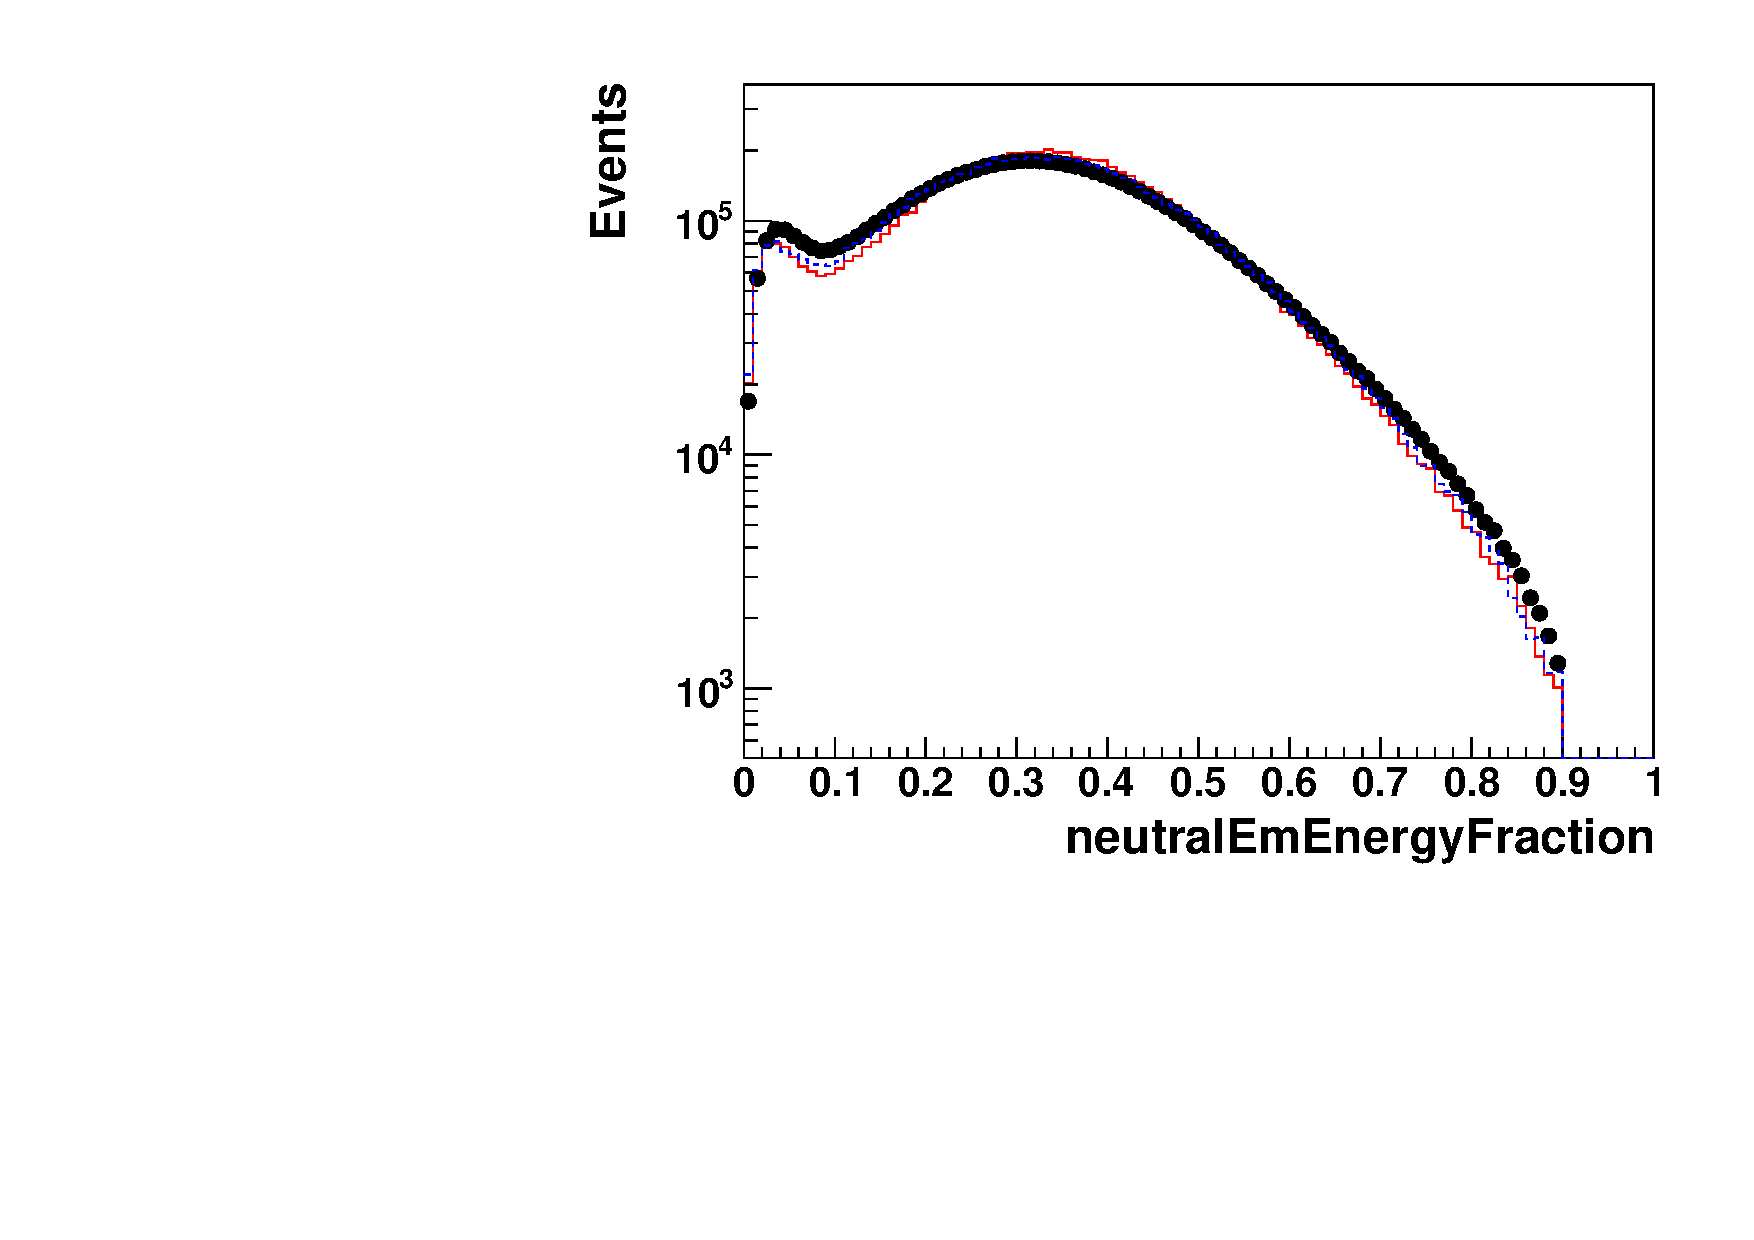
\includegraphics{EXO-12-024/figs/Data-MC-comparisons/neutralEmEnergyFractionlog.pdf}} \\
\end{tabular}
  \caption[Leading two jets mass drop]{Comparisons between data and Monte Carlo for neutral eletromagnetic energy fraction.  
	   The MC is normalized to the number of data events. Plot on the right is the log scale plot. (The plot includes only a subset of the full data sample.)}
  \label{fig:neutralEmEnergyFraction}
\end{figure}

\begin{figure}[htb]
\centering
\begin{tabular}{cc}
     \resizebox{0.5\linewidth}{!}{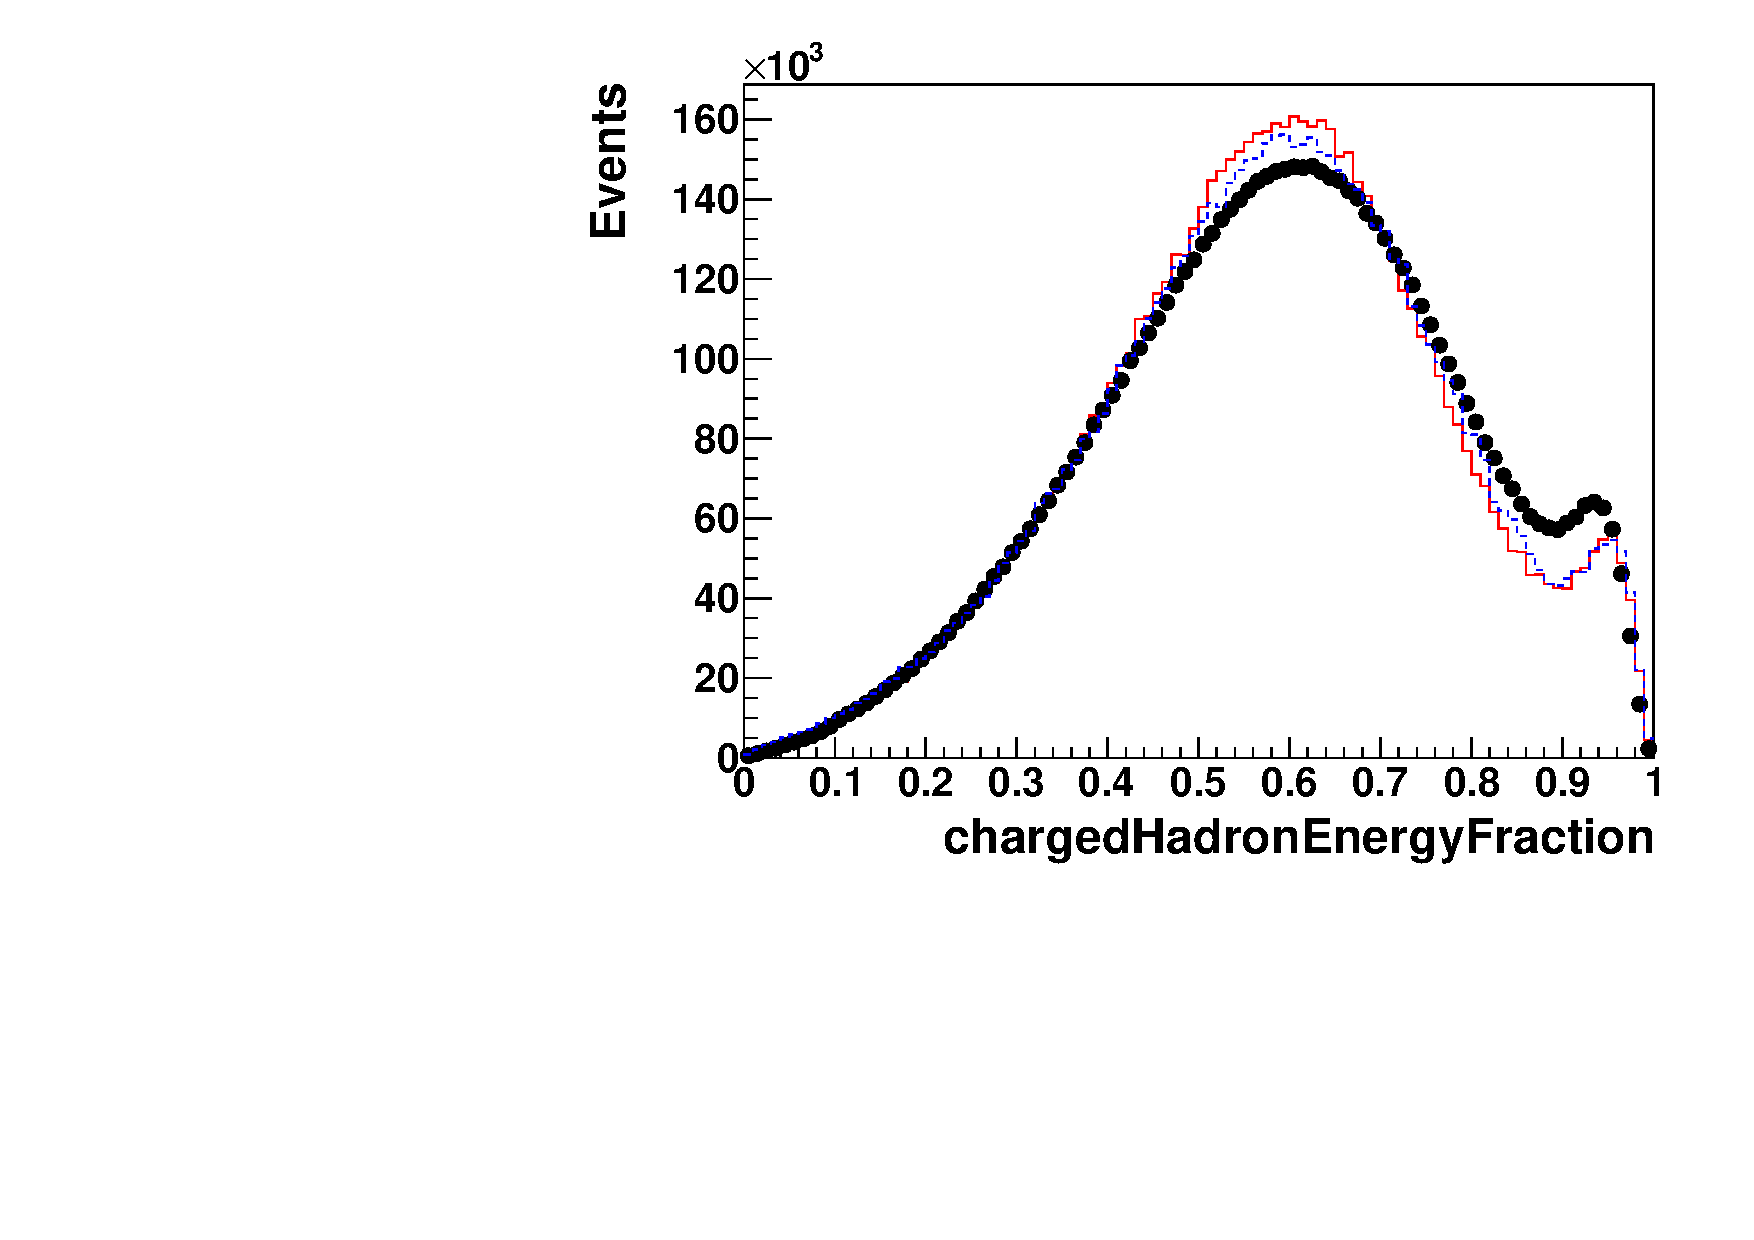
\includegraphics{EXO-12-024/figs/Data-MC-comparisons/chargedHadronEnergyFraction.pdf}} &
     \resizebox{0.5\linewidth}{!}{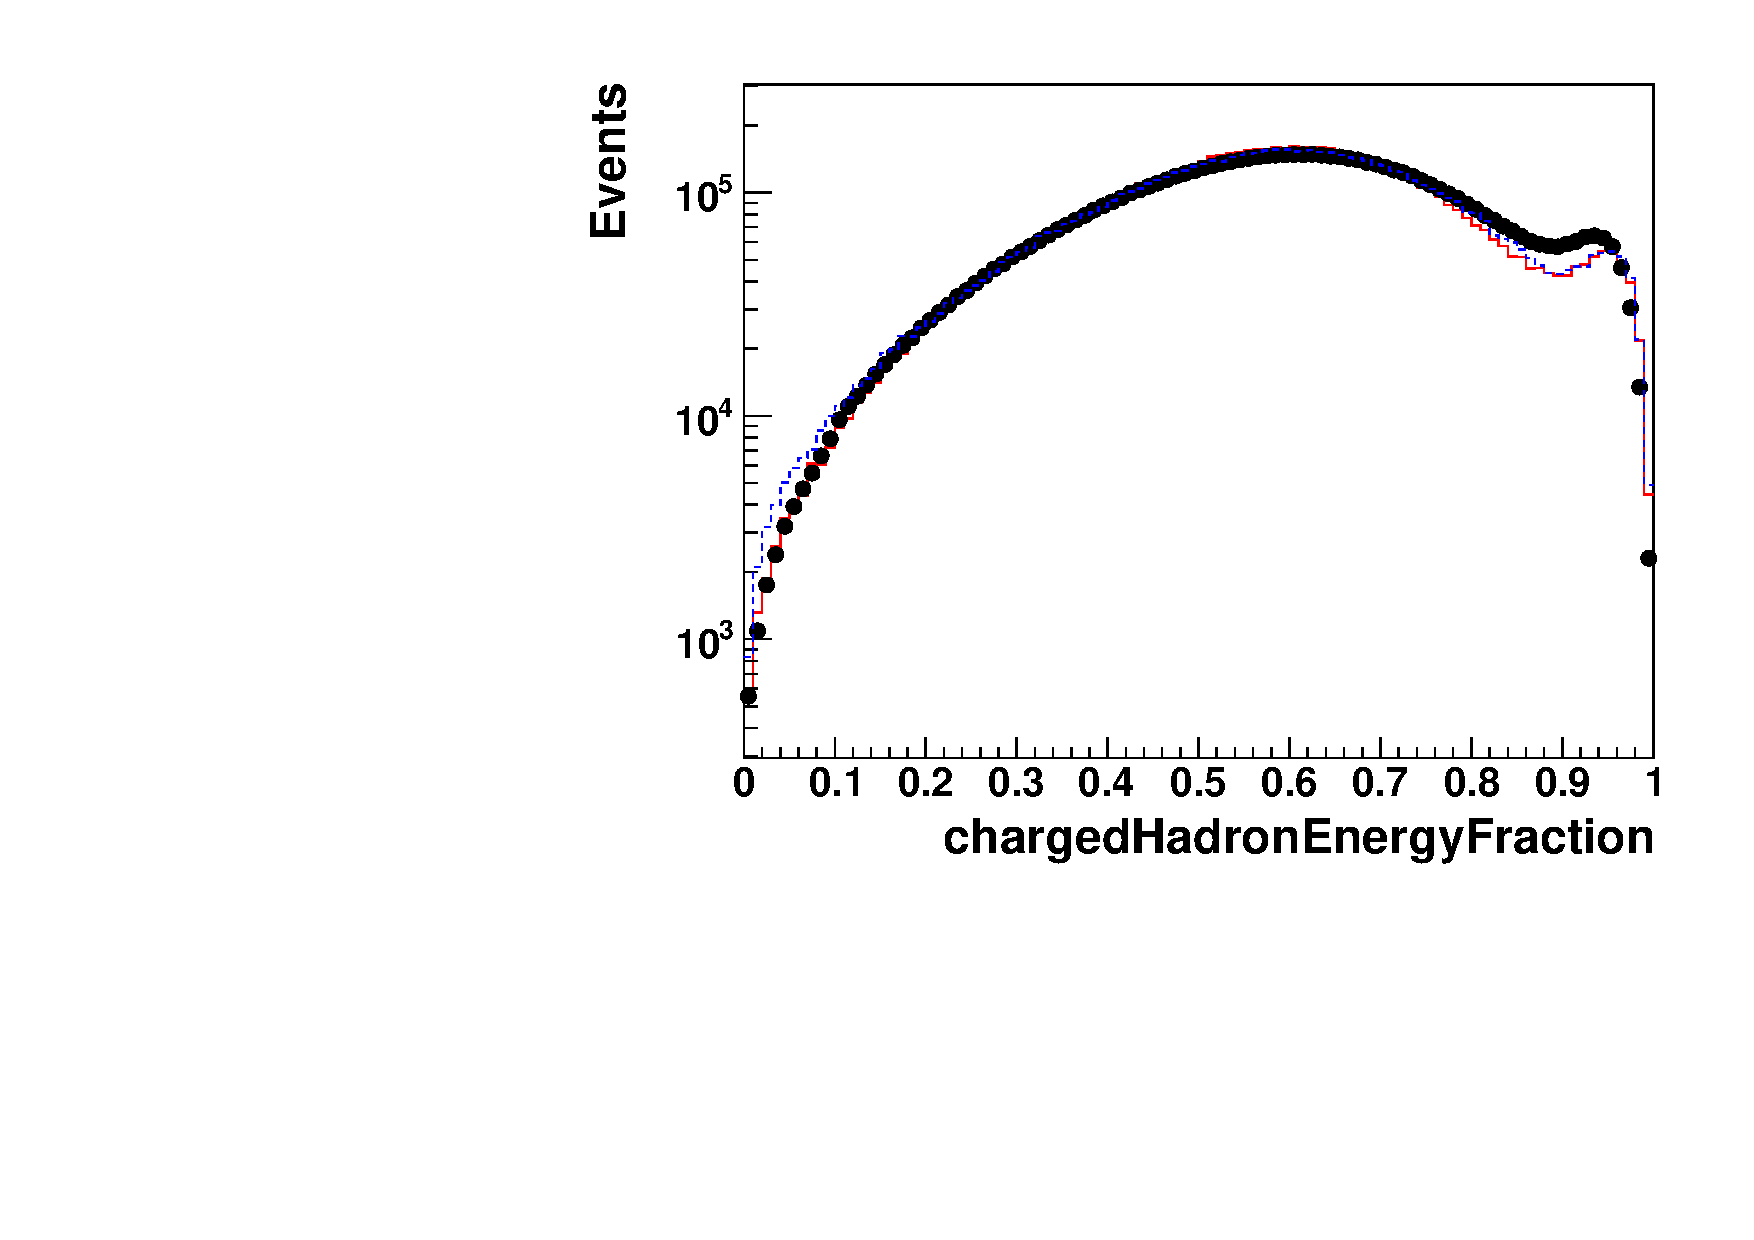
\includegraphics{EXO-12-024/figs/Data-MC-comparisons/chargedHadronEnergyFractionlog.pdf}} \\
\end{tabular}
  \caption[Leading two jets mass drop]{Comparisons between data and Monte Carlo for charged hadron energy fraction.  
	   The MC is normalized to the number of data events. Plot on the right is the log scale plot. (The plot includes only a subset of the full data sample.)}
  \label{fig:chargedHadronEnergyFraction}
\end{figure}

\newpage


\begin{figure}[htb]
\centering
\begin{tabular}{cc}
     \resizebox{0.5\linewidth}{!}{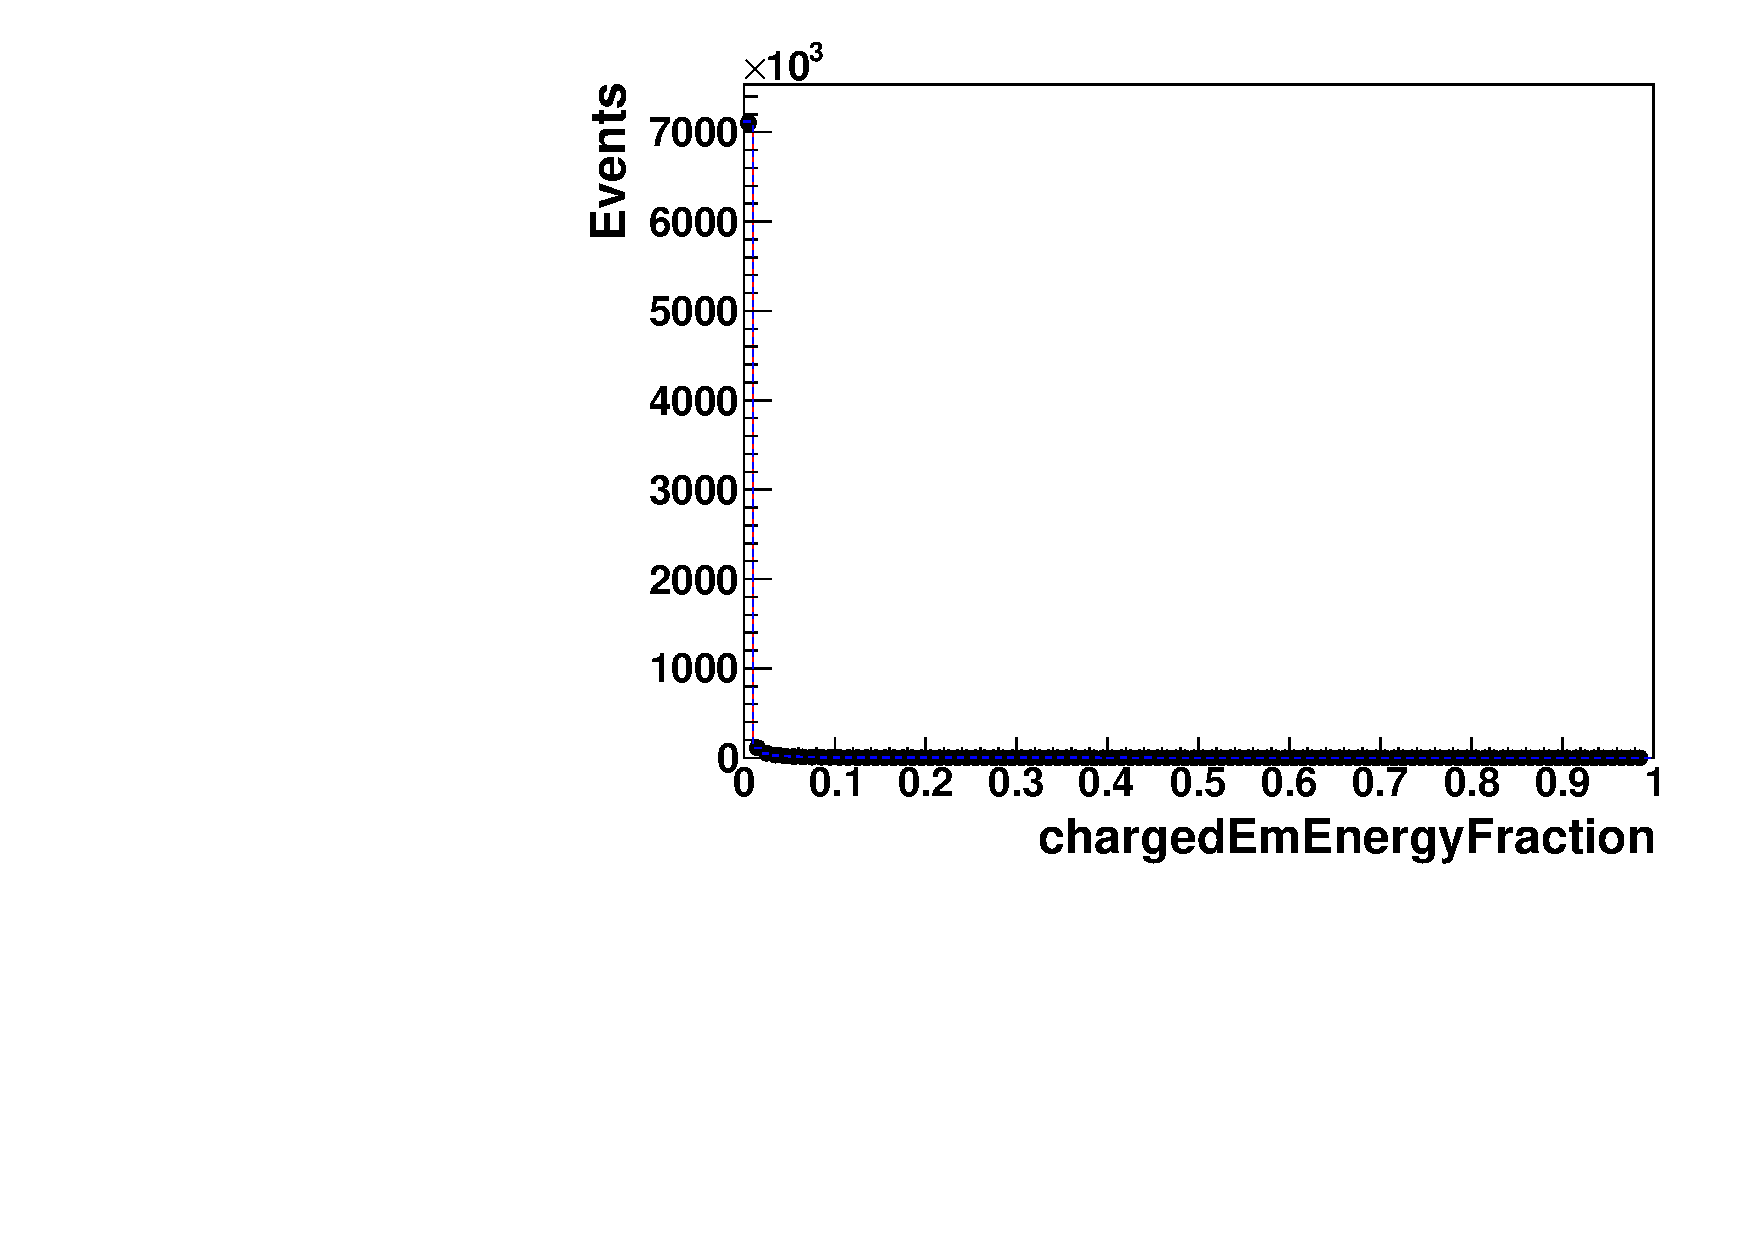
\includegraphics{EXO-12-024/figs/Data-MC-comparisons/chargedEmEnergyFraction.pdf}} &
     \resizebox{0.5\linewidth}{!}{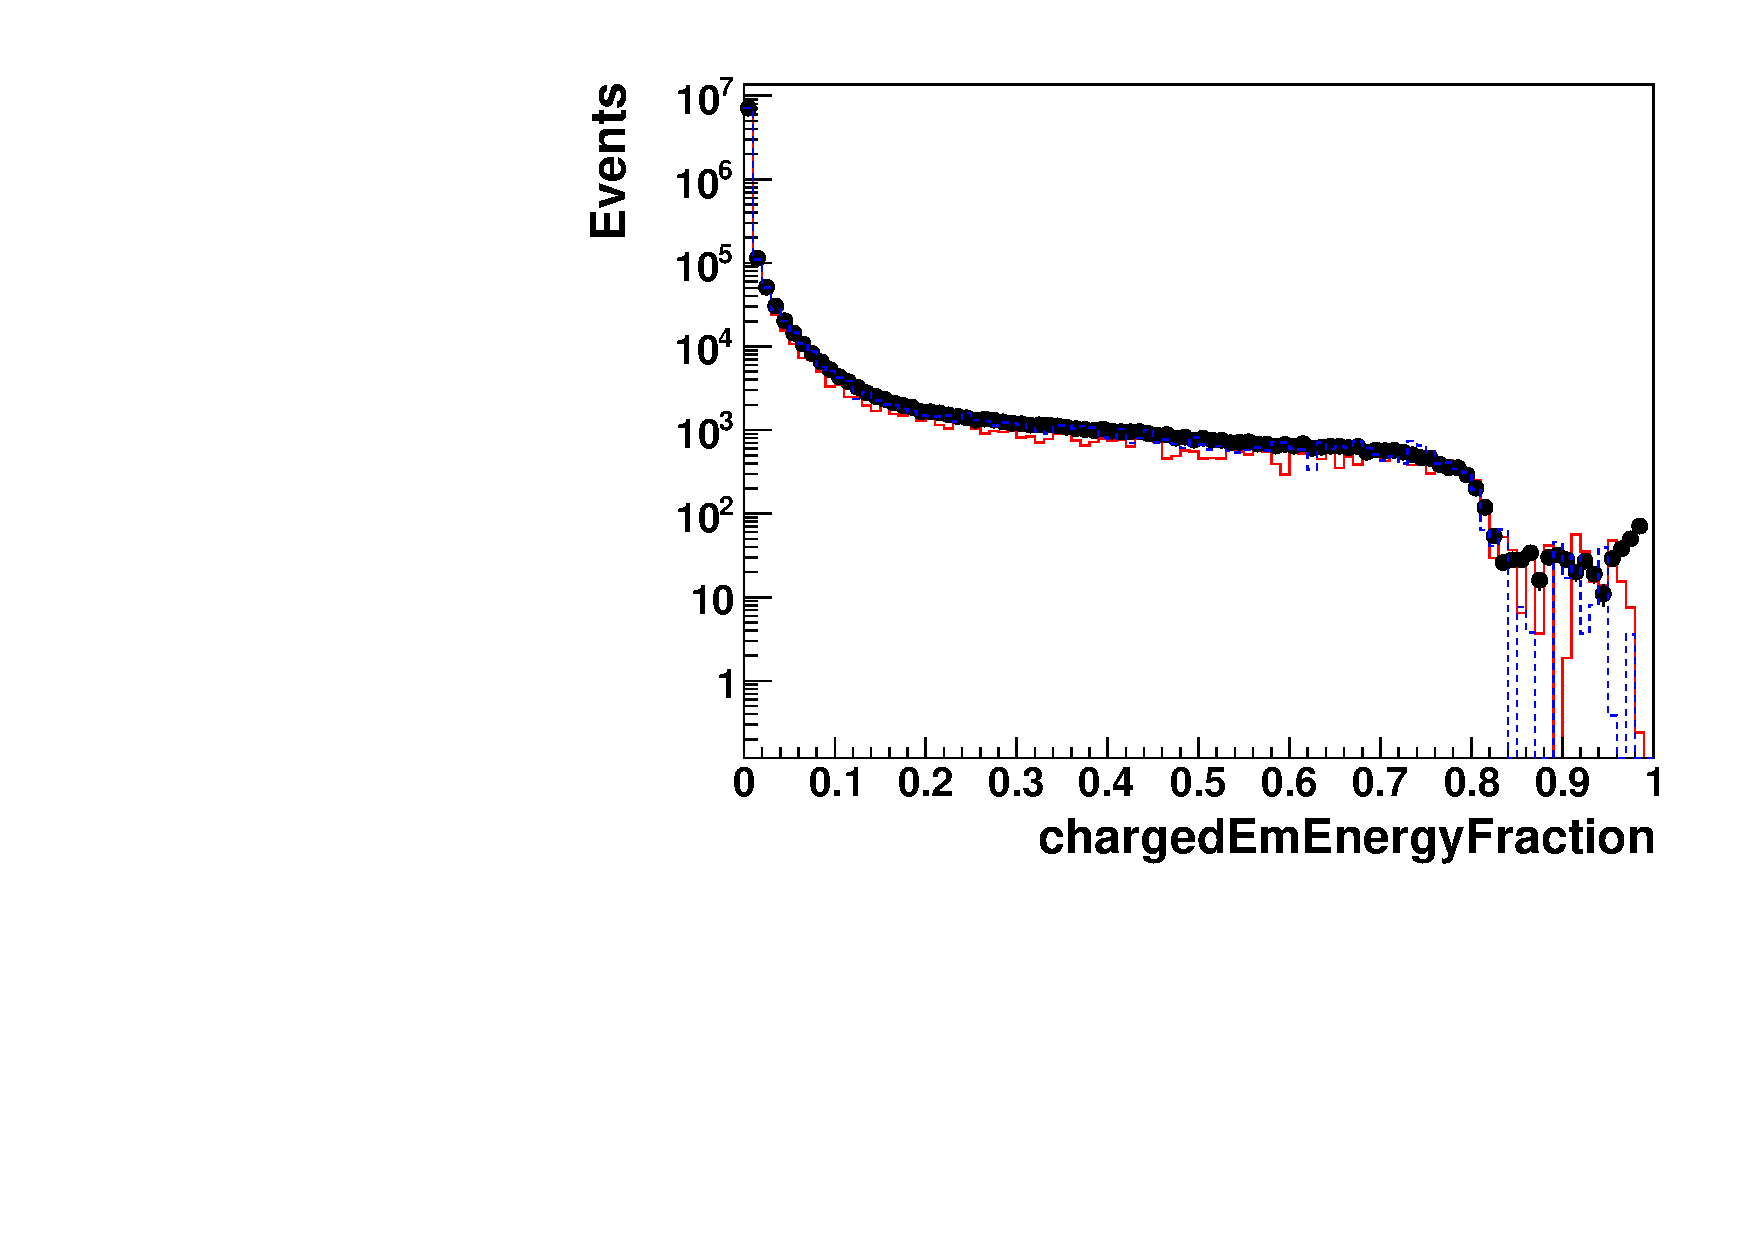
\includegraphics{EXO-12-024/figs/Data-MC-comparisons/chargedEmEnergyFractionlog.pdf}} \\
\end{tabular}
  \caption[Leading two jets mass drop]{Comparisons between data and Monte Carlo for charged eletromagnetic energy fraction.  
	   The MC is normalized to the number of data events. Plot on the right is the log scale plot. (The plot includes only a subset of the full data sample.)}
  \label{fig:chargedEmEnergyFraction}
\end{figure}

\begin{figure}[htb]
\centering
\begin{tabular}{cc}
     \resizebox{0.5\linewidth}{!}{\includegraphics{EXO-12-024/figs/Data-MC-comparisons/chargedMultiplicity.pdf}} &
     \resizebox{0.5\linewidth}{!}{\includegraphics{EXO-12-024/figs/Data-MC-comparisons/chargedMultiplicitylog.pdf}} \\
\end{tabular}
  \caption[Leading two jets mass drop]{Comparisons between data and Monte Carlo for charged multiplicity.  
	   The MC is normalized to the number of data events. Plot on the right is the log scale plot. (The plot includes only a subset of the full data sample.)}
  \label{fig:chargedMultiplicity}
\end{figure}

\newpage

\begin{figure}[htb]
\centering
\begin{tabular}{cc}
     \resizebox{0.5\linewidth}{!}{\includegraphics{EXO-12-024/figs/Data-MC-comparisons/nConstituents.pdf}} &
     \resizebox{0.5\linewidth}{!}{\includegraphics{EXO-12-024/figs/Data-MC-comparisons/nConstituentslog.pdf}} \\
\end{tabular}
  \caption[Leading two jets mass drop]{Comparisons between data and Monte Carlo for number of constituents.  
	   The MC is normalized to the number of data events. Plot on the right is the log scale plot. (The plot includes only a subset of the full data sample.)}
  \label{fig:nConstituents}
\end{figure}


\begin{figure}[htb]
\centering
\begin{tabular}{cc}
     \resizebox{0.5\linewidth}{!}{\includegraphics{EXO-12-024/figs/Data-MC-comparisons/muonEnergyFraction.pdf}} &
     \resizebox{0.5\linewidth}{!}{\includegraphics{EXO-12-024/figs/Data-MC-comparisons/muonEnergyFractionlog.pdf}} \\
\end{tabular}
  \caption[Leading two jets mass drop]{Comparisons between data and Monte Carlo for the muon energy fraction of the leading two jets.  
	   The MC is normalized to the number of data events. Plot on the right is the log scale plot. (The plot includes only a subset of the full data sample.)}
  \label{fig:muonEnergyFraction}
\end{figure}

\newpage


%We find that the QCD MC agrees with data, although not perfect.
%For the dijet kinematics shown in Fig~\ref{fig:mjj},\ref{fig:dy},\ref{fig:dphi},\ref{fig:metSumPt},\ref{fig:jet1-pt},\ref{fig:jet2-pt},\ref{fig:eta of leading jet} and \ref{fig:eta of second leading jet}, we observe better agreement of Pythia6 $Z2*$ than Herwig++.
%For the jet substructure variables shown in Fig~\ref{fig:mass of leading two jets},\ref{fig:mass drop of leading two jets} and \ref{fig:subjet dR of leading two jets}, we observe that Herwig++ is better than Pythia $Z2*$.  
%In summary, Pythia6 $Z2*$ is more accurate at modelling the dijet kinematics,
%while Herwig++ models better the jet substructure.
We find that the QCD MC agrees with data, although not perfect.
For the dijet kinematics and also the jet substructure variables, we observe about the same agreement of \PYTHIA~6 and \HERWIG{++}. 
For this analysis, we chose to model the background shape from the data itself
(as described below)
and depend on QCD MC only to provide us guidance and a cross check.

Figure~\ref{fig:dphiSingle}, Figure~\ref{fig:dphiDouble} and Figure~\ref{fig:metSumPtSingle} are particulariy useful to identify jets from calorimenter noise which would show up at low values of $\Delta\phi$ and high values of $E_{T}^{miss}/\sum E_{T}$. No enhencement in this region is observed which gives confidence that the applied noise filterd and jet ID cuts leave no noise contamination within the two leading jets.

%Fig~\ref{fig:CA8Single} and Fig~\ref{fig:CA8Double} show the $\Delta \phi$ between the leading ungroomed CA8 jet and leading pruned CA8 jet.

%\begin{table}[htb]
%\begin{center}
%\begin{tabular}{|p{2.5cm}|p{2.5cm}|p{2.5cm}|p{2.5cm}|p{2.5cm}|}
%\begin{tabular}{|c|c|c|c|}
%\hline
%Categories & $\Delta \phi < 0.5(\%) $  & $0.5 < \Delta\phi < 2.0 (\%)$ & $2.0 < \Delta\phi (\%)$ \\
%\hline
%low purity 1-tag& 51.067 & 0.003 & 48.930 \\
%medium purity 1-tag&  90.458 & 0.002 & 9.541 \\
%high purity 1-tag & 95.156 & 0.001 & 4.844\\
%low purity 2-tag &  89.332 & 0.004 & 10.664 \\
%medium purity 2-tag& 90.636 & 0 & 9.363\\
%high purity 2-tag &  92.585 & 0 & 7.415\\
%\hline
%\end{tabular}
%\end{center}
%\caption{The ratio of the leading ungroomed CA8 jet matching to the leading pruned CA8 jet in different categories.}
%\label{table:matching}
%\end{table}


%Table~\ref{table:matching} shows the matching of the leading ungroomed CA8 jet and the leading pruned CA8 jet. 
%In the case of  $\Delta \phi<0.5$, the leading ungroomed CA8 jet  and leading pruned CA8 jet match.
%In the case of  $0.5 < \Delta \phi<2.0$, the leading ungroomed CA8 jet  and leading pruned CA8 jet don't match at all.
%In the case of  $\Delta \phi > 2.0$, the leading two jets are swapped and the leading ungroomed CA8 jet matches to the second leading pruned CA8 jet.

%Therefore there is no significant impact on the analyis from the fact that we use the leading two ungroomed CA8 jets to reconstruct the dijet mass while using the leading two pruned CA8 jets for W/Z-tagging of events.

Figure~\ref{fig:npv} shows the number of primary vertices distribution after pile up reweighting on the MC. 
Figures~\ref{fig:neutralHadronEnergyFraction},~\ref{fig:neutralEmEnergyFraction},~\ref{fig:chargedHadronEnergyFraction},~\ref{fig:chargedEmEnergyFraction},~\ref{fig:chargedMultiplicity} and~\ref{fig:nConstituents} show the jet ID variable distribution after the event selection, and Figure~\ref{fig:muonEnergyFraction} shows the muon energy faction of the leading two jets.

\clearpage
